% Dieses Dokument muss mit PDFLatex geestzt werden
% Vorteil: Grafiken koennen als jpg, png, ... verwendet werden
%          und die Links im Dokument sind auch gleich richtig
%
\documentclass[
               paper=a4,,
%               twoside, % fuer die Betrachtung am Schirm ungeschickt
% Optionen fuer typearea.
               BCOR1.92mm,DIV12,headinclude, %je hoeher der DIV-Wert, desto mehr geht auf eine Seite - Hack f�r BCOR. Bei BCOR2mm sind die Fuellpunkte beim Inhaltsverzeichnis falsch
%               titlepage,
               bibliography=totoc,
%               idxtotoc,   %Index ins Inhaltsverzeichnis
%				liststotoc, %List of X ins Inhaltsverzeichnis, mit liststotocnumbered werden die Abbildungsverzeichnisse nummeriert
               headsepline,
               cleardoublepage=empty,
               parskip=half,
%				pointlessnumbers, %f"ur englische Texte, dann auch "packages_and_options" und "fonts" anpassen.
%               draft    % um zu sehen, wo noch nachgebessert werden muss - wichtig, da Bindungskorrektur mit drin
               final   % ACHTUNG! - in pagestyle.tex noch Seitenstil anpassen
               ]{scrbook}

%Englisch:			   
%\let\ifdeutsch\iffalse
%\let\ifenglisch\iftrue

%Deutsch:
\let\ifdeutsch\iftrue
\let\ifenglisch\iffalse

			   
% $Id: packages_and_options.tex 65 2012-04-23 20:50:44Z koppor $

%%%
% Beschreibung:
% In dieser Datei werden zuerst die benoetigten Pakete eingebunden und
% danach diverse Optionen gesetzt. Achtung Reihenfolge ist entscheidend!
%
%%%


%%%
% Styleguide:
%
% Ein sehr kleiner Styleguide. Packages werden in Blöcken organisiert.
% Ein Block beginnt mit drei % in einer Zeile, dann % <Blocküberschrift>, dann 
% eine Liste der möglichen Optionen und deren Einstellungen, Gründe und Kommentare
% eine % Zeile in der sonst nichts steht und dann wieder %%% in einer Zeile.
%
% Zwischen zwei Blöcken sind 2 Leerzeilen!
% Zu jedem Paket werden soviele Optionen wie möglich/nötig angegeben
%
%%%


%%%
%Parallelbetrieb tex4ht und pdflatex
\makeatletter
\@ifpackageloaded{tex4ht}{\def\iftex4ht{\iftrue}}
                         {\def\iftex4ht{\iffalse}}
\makeatother
%%%


%%%
%Farbdefinitionen
\usepackage[hyperref,dvipsnames]{xcolor}
%


%%%
% Neue deutsche Rechtschreibung und Literatur statt "Literature", Nachfolger von ngerman.sty
\ifdeutsch
\usepackage[ngerman]{babel}
  %Ein "abstract" ist eine "Kurzfassung", keine "Zusammenfassung"
  \addto\captionsngerman{%
    \renewcommand\abstractname{Kurzfassung}%
  }
\else
%
%
% if you are writing in english
% für englische Texte, Hinweise zu weiteren, notwendigen Umstellungen in README.txt beachten
\usepackage[american]{babel}
\fi
%
%%%


%%%
% Codierung
% Wir sind im 21 Jahrhundert, utf-8 löst so viele Probleme.
%
% Mit UTF-8 funktionieren folgende Pakete nicht mehr. Bitte beachten!
%   * fancyvrb mit § 
%   * easylist -> http://www.ctan.org/tex-archive/macros/latex/contrib/easylist/ 
\usepackage[utf8]{inputenc}
%
%%%


%%%
% erweitertes Enumerate
\usepackage{paralist}
%
%%%


%%%
% fancyheadings (nicht nur) fuer koma
\usepackage[automark]{scrpage2} 
%
%%%


%%%
% Versionskontrolle
%SVN. Für die final version "draft" durch "final" ersetzen
\iftex4ht
\usepackage[final,eso-foot]{svninfo}
\else
\usepackage[draft,eso-foot]{svninfo}
\fi
%
%Falls rcs oder cvs als Versionskontrolle verwendet wird, dann anstattdessen
%\usepackage{rcs}
%verwenden
%
%%%


%%%
%Mathematik
%
\usepackage[fleqn,leqno]{amsmath} % Viele Mathematik-Sachen: Doku: /usr/share/doc/texmf/latex/amsmath/amsldoc.dvi.gz
%fleqn (=Gleichungen linksbündig platzieren) funktioniert nicht direkt. Es muss noch ein Patch gemacht werden:
\addtolength\mathindent{1em}%work-around ams-math problem with align and 9 -> 10
\usepackage{mathtools} %fixes bugs in AMS math
%
%%%


%%%
% Intelligentes Leerzeichen um hinter Abkürzungen die richtigen Abstände zu erhalten, auch leere.
% siehe commands.tex \gq{}
\usepackage{xspace}
%
%%%


%%%
% Anhang
\usepackage{appendix}
%[toc,page,title,header]
%
%%%


%%%
% Grafikeinbindungen
\usepackage{graphicx}%Parameter "pdftex" unnoetig
\graphicspath{{graphics/}}
%
%%%


%%%
% Tabellenerweiterungen
\usepackage{array} %increases tex's buffer size and enables ``>'' in tablespecs
\usepackage{longtable}
%
%%%

%%%
% Eine Zelle, die sich über mehrere Zeilen erstreckt.
% Siehe Beispieltabelle in Kapitel 2
\usepackage{multirow}
%
%%%


%%%
% Links verhalten sich so, wie sie sollen
\usepackage{url}
%
%%%


%%%
% Index über Begriffe, Abkürzungen
%\usepackage{makeidx} makeidx ist out -> http://xindy.sf.net verwenden
%
%%%

%%%
%lustiger Hack fuer das Abkuerzungsverzeichnis
%nach latex durchlauf folgendes ausfuehren
%makeindex ausarbeitung.nlo -s nomencl.ist -o ausarbeitung.nls 
%danach nochmal latex
%\usepackage{nomencl}
%	\let\abk\nomenclature %Deutsche Ueberschrift setzen
%	  	\renewcommand{\nomname}{List of Abbreviations}
%		%Punkte zw. Abkuerzung und Erklaerung
%	  	\setlength{\nomlabelwidth}{.2\hsize}
%	  	\renewcommand{\nomlabel}[1]{#1 \dotfill}
%		%Zeilenabstaende verkleinern
%	  	\setlength{\nomitemsep}{-\parsep}
%	\makenomenclature
%
%%%

%%%
% Logik für Tex
\usepackage{ifthen} %fuer if-then-else @ commands.tex
%
%%%


%%%
% unterschiedliche Fancy-Chapter-Styles
%\usepackage[Bjarne]{fncychap}
%\usepackage[Lenny]{fncychap}
%
%%%


%%%
% Deckblattstyle
\usepackage[]{diplomtitel/diplomtitel}
%
%%%


%%%
%
\usepackage{listings}
%
%%%


%%%
%Alternative zu Listings ist fancyvrb. Kann auch beides gleichzeitig benutzt werden.
\usepackage{fancyvrb}
%\fvset{fontsize=\small} %Groesse fuer den Fliesstext. Falls deaktiviert: \normalsize
%Funktioniert mit UTF-8 nicht mehr
%\DefineShortVerb{\§} %Somit kann im Text ganz einfach |verbatim| text gesetzt werden.
\RecustomVerbatimEnvironment{Verbatim}{Verbatim}{fontsize=\footnotesize}
\RecustomVerbatimCommand{\VerbatimInput}{VerbatimInput}{fontsize=\footnotesize}
%
%%%


%%%
% Bildunterschriften bei floats genauso formatieren wie bei Listings
% Anpassung wird unten bei den newfloat-Deklarationen vorgenommen
% Caption2 vielleicht besser
\usepackage{caption}
%
%%%


%%%
% Ermoeglicht es, Abbildungen um 90 Grad zu drehen
% Alternatives Paket: rotating Allerdings wird hier nur das Bild gedreht, während bei lscape auch die PDF-Seite gedreht wird. 
%Das Paket lscape dreht die Seite auch nicht 
\usepackage{pdflscape}
%
%%%


%%%
% Fuer listings
% Wird für fancyvrb und für lstlistings verwendet
% zustäzlich für den Paramter [H] = Floats WIRKLICH da wo sie deklariert wurden paltzieren - ganz ohne Kompromisse
% floatrow ist der Nachfolger von float
\iftex4ht
\usepackage{float}
\else
%tex4ht is not compatible with the advanced floatrow package
\usepackage{floatrow} 
\fi
%
%%%


%%%
% Fuer Abbildungen innerhalb von Abbildungen
% Ersetzt das Paket subfigure
%\usepackage{subfig}
%
%%%


%%%
%Fuer Tabellen mit Variablen Spaltenbreiten
%\usepackage{tabularx}
%\usepackage{tabulary}
%
%%%


%%%
% Fußnoten
% 
%\usepackage{dblfnote}  %Zweispaltige Fußnoten
%
% Keine hochgestellten Ziffern in der Fußnote (KOMA-Script-spezifisch):
%\deffootnote[1.5em]{0pt}{1em}{\makebox[1.5em][l]{\bfseries\thefootnotemark}} 
%
% Abstand zwischen Fußnoten vergrößern:
%\setlength{\footnotesep}{.85\baselineskip}
%
%
\renewcommand{\footnoterule}{}             % Keine Trennlinie zur Fußnote 
\addtolength{\skip\footins}{\baselineskip} % Abstand Text <-> Fußnote
% Fußnoten immer ganz unten auf einer \raggedbottom-Seite
\usepackage{fnpos}
%
%%%


%%%
%
\raggedbottom     % Variable Seitenhöhen zulassen
%
%%%


%%%
% Falls die Seitenzahl bei einer Referenz auf eine Abbildung nur dann angegeben werden soll,
% falls sich die Abbildung nicht auf der selben Seite befindet...
\iftex4ht
%tex4ht does not work well with vref, therefore we emulate vref behavior
\newcommand{\vref}[1]{\ref{#1}}
\else
\ifdeutsch
\usepackage[ngerman]{varioref}
\else
\usepackage{varioref}
\fi
\fi
%%%

%%%
% Noch schoenere Tabellen als mit booktabs mit http://www.zvisionwelt.de/downloads.html
\usepackage{booktabs} 
%
%\usepackage[section]{placeins}
%
%%%


%%%
%Fuer Graphiken. Allerdings funktioniert es nicht zusammen mit pdflatex
%\usepackage{gastex} % \tolarance kann dann nicht mehr umdefiniert werden
%
%%%


%%%
%
%\usepackage{multicol}
%\usepackage{setspace} % kollidiert mit diplomarbeit.sty
%
%http://www.tex.ac.uk/cgi-bin/texfaq2html?label=floats
%\usepackage{flafter} %floats IMMER nach ihrer Deklaration platzieren
%
%%%


%%%
%schoene TODOs
\usepackage{todonotes}
%
%%%


%%%
% Neue Pakete bitte VOR hyperref einbinden. Insbesondere bei Verwendung des
% Pakets "index" wichtig, da sonst die Referenzierung nicht funktioniert.
% Für die Indizierung selbst ist unter http://xindy.sourceforge.net
% ein gutes Tool zu erhalten 
%%%


%%%
%
% hier also neue packages einbinden
%
%%%


%%%
% ggf.in der Endversion komplett rausnehmen. dann auch \href in commands.tex aktivieren
% Alle Optionen nach \hypersetup verschoben, sonst crash
%
\usepackage[]{hyperref}%siehe auch: "Praktisches LaTeX" - www.itp.uni-hannover.de/~kreutzm
%
%% Da es mit KOMA 3 und xcolor zu Problemen mit den global Options kommt MÜSSEN die Optionen so gesetzt werden.
%

% Eigene Farbdefinitionen ohne die Namen des xcolor packages
\definecolor{darkblue}{rgb}{0,0,.5}
\definecolor{black}{rgb}{0,0,0}

\hypersetup{
	breaklinks=true,
	bookmarksnumbered=true,
	bookmarksopen=true,
	bookmarksopenlevel=1,
	breaklinks=true,
	colorlinks=true,
	pdfstartview=Fit,
	pdfpagelayout=SinglePage,
	%
	filecolor=darkblue,
	urlcolor=darkblue,
	linkcolor=black,
	citecolor=black
}
%
%%%


%%%
% Zur Darstellung von Algorithmen
% Algorithm muss nach hyperref geladen werden
\usepackage[chapter]{algorithm} 
\usepackage[]{algpseudocode}
%
%%%


%%%
% Schriften
%%%
%
\automark[section]{chapter}
\setkomafont{pageheadfoot}{\normalfont\sffamily}
\setkomafont{pagenumber}{\normalfont\rmfamily}
%\setheadsepline[.4pt]{.4pt} %funktioniert nicht: Alle Linien sind hier weg
%
%%%

%%%
%
\ifenglisch
% Fuer englische Texte sind serifenhafte Ueberschriften gut. Deshalb hier der Befehl zum Aktivieren von serifenhaften Ueberschriften
\setkomafont{disposition}{\normalfont\rmfamily}

% Bei englisschen Texten das Label (optionaler Eintrag bei \item) bei description-Umgegungen nur auf fett und nicht fett+serifenlos stellen.
\setkomafont{descriptionlabel}{\normalfont\bfseries}
\fi
%
%%%

%%%
% Fuer deutsche Texte: Weniger Silbentrennung, mehr Abstand zwischen den Woertern
\ifdeutsch
\setlength{\emergencystretch}{3em} % Silbentrennung reduzieren durch mehr frei Raum zwischen den Worten
\fi
%%%

%Symbole
%--------
%\usepackage[geometry]{ifsym} % \BigSquare
%\usepackage{mathabx}
%\usepackage{stmaryrd} %fuer \ovee, \owedge, \otimes
%\usepackage{marvosym} %fuer \Writinghand %patched to not redefine \Rightarrow
%\usepackage{mathrsfs} %mittels \mathscr{} schoenen geschwungenen Buchstaben erzeugen
%\usepackage{calrsfs} %\mathcal{} ein bisserl dickeren buchstaben erzeugen - sieht net so gut aus.
                      %durch mathpazo ist das schon definiert
\usepackage{amssymb}

%name-clashes von marvosym und mathabx vermeiden:
\def\delsym#1{%
%  \expandafter\let\expandafter\origsym\expandafter=\csname#1\endcsname
%  \expandafter\let\csname orig#1\endcsname=\origsym
  \expandafter\let\csname#1\endcsname=\relax
}

%\usepackage{pifont}
%\usepackage{bbding}
%\delsym{Asterisk}
%\delsym{Sun}\delsym{Mercury}\delsym{Venus}\delsym{Earth}\delsym{Mars}
%\delsym{Jupiter}\delsym{Saturn}\delsym{Uranus}\delsym{Neptune}
%\delsym{Pluto}\delsym{Aries}\delsym{Taurus}\delsym{Gemini}
%\delsym{Rightarrow}
%\usepackage{mathabx} - Ueberschreibt leider zu viel - und die \le-Zeichen usw. sehen nicht gut aus!


%Fallback-Schriftart
%\usepackage{lmodern}  % Latin Modern Fonts sind die Nachfolger von Computer Modern, den LaTeX-Standardfonts
%Quelle: http://homepage.ruhr-uni-bochum.de/Georg.Verweyen/pakete.html
%Allerdings sieht diese Schritart in Diplomarbeiten fuer Fliesstext auch nicht besonders schoen aus.
%Trotzdem ist sie fuer Programmcode gut geeignet

%Schriftart fuer die Ueberschriften - ueberschreibt lmodern
\ifdeutsch
\usepackage[scaled=.95]{helvet}
\else
\usepackage[scaled=.90]{helvet}
\fi

%Schriftart fuer Programmcode - ueberschreibt lmodern
%Falls auskommentiert, wird die Standardschriftart genommen
%\usepackage[scaled=.92]{luximono} % Fuer schreibmaschinenartige Schluesselwoerter in den Listings - geht bei alten Installationen nicht, da einige Fontshapes (<>=) fehlen
%\usepackage{courier} 

% Tolle Schriften...
%\usepackage{helvet}
%\usepackage{palatino}
%\usepackage[osf]{libertine}
% Für Schreibschrift würde tun, muss aber ned
%\usepackage{mathrsfs} %  \mathscr{ABC}


%Schriftart fuer den Fliesstext - ueberschreibt lmodern
%
\ifdeutsch
\usepackage[osf]{mathpazo} %ftp://ftp.dante.de/tex-archive/fonts/mathpazo/ - Tipp aus DE-TEX-FAQ 8.2.1
\fi
%Bringt Palantino, osf = Minuskel-Ziffern
%
%\usepackage{charter} %Charter fuer englsiche Texte
%\linespread{1.05} % Durchschuss für Charter leicht erhöhen
%
%\usepackage{mathptmx} %Times fuer englische Texte. Sieht nicht sooo gut aus.
\ifenglisch
\usepackage{lmodern}
\fi

\usepackage[T1]{fontenc}


% optischer Randausgleich - bei miktex gleich dabei - bei linux von
%  http://www.ctan.org/tex-archive/macros/latex/contrib/microtype/
%  herunterladen 
\usepackage{microtype}
%Falls bei einer Silbentrennung ploetzlich eine ganze Zeile fehlt (passiert unter Windows XP mit MikTex 2.5 und foxit reader als pdfreader
%\usepackage{pdfcprot}
%ausprobieren. Dieses erzeugt allerdings nur für Palatino (in dieser Vorlage die Default-Schrift) einen guten optischen Randausgleich
%Falls alle Stricke reissen, muss leider auf den optischen Randausgleich verzichtet werden.

%fuer microtype
%tracking=true muss als Parameter des microtype-packages mitgegeben werden
%
%Deaktiviert, da dies bei Algorithmen seltsam aussieht
%
%\DeclareMicrotypeSet*[tracking]{my}{ font = */*/*/sc/* }% 
%\SetTracking{ encoding = *, shape = sc }{ 45 }% Hier wird festgelegt,
            % dass alle Passagen in Kapitälchen automatisch leicht
            % gesperrt werden.
			% Quelle: http://homepage.ruhr-uni-bochum.de/Georg.Verweyen/pakete.html

%
%%%


%%%
%Bugfixes packages
\usepackage{fixltx2e} %Bereinigt einige Ungereimtheiten, die auf Grund von Rueckwaertskompatibilitaet beibahlten wurden.
%\usepackage{mparhack} %Fixt die Position von marginpars (die in DAs selten bis gar nicht gebraucht werden}
%\usepackage{ellipsis} %Fixt die Abstaende vor \ldots. Wird wohl auch nicht benoetigt.
%
%%%


%%%
% Rand                                                                       %
%Viele Moeglichkeiten, die Raender im Dokument einzustellen.
%Satzspiegel neu berechnen. Dokumentation dazu ist in "scrguide.pdf" von KOMA-Skript zu finden
%  Optionen werden bei \documentclass[] in ausarbeitung.tex mitgegeben.
\typearea[current]{current} %neu berechnen, da neue Schrift eingebunden

%\usepackage{a4}
%\usepackage{a4wide}
%\areaset{170mm}{277mm} %a4:29,7hochx21mbreit

%Wer die Masse direkt eingeben moechte:
%Bei diesem Beispiel wird die Regel nicht beachtet, dass der innere Rand halb so gross wie der aussere Rand und der obere Rand halb so gross wie der untere Rand sein sollte
%\usepackage[inner=2.5cm, outer=2.5cm, includefoot, top=3cm, bottom=1.5cm]{geometry}



%
%%%


%%%
% Optionen                                                                  
%
%Skip=0 funktioniert nicht
\captionsetup{format=hang,labelfont=bf,justification=justified,singlelinecheck=false,skip=0pt}
%
%neue float Umgebung fuer Listings, die mittels fancyvrb gesetzt werden sollen
\floatstyle{ruled}
\newfloat{Listing}{tbp}{code}[chapter]
\newfloat{Algorithmus}{tbp}{alg}[chapter]
%
%amsmath
%\numberwithin{equation}{section}
%\renewcommand{\theequation}{\thesection.\Roman{equation}}
%
%pdftex
\pdfcompresslevel=9
%
%Tabellen (array.sty)
\setlength{\extrarowheight}{1pt}
%
%

% Andere Kapitelueberschriften
% falls einem der Standard von KOMA nicht gefaellt...
% Falls man zurück zu KOMA moechte, dann muss jede der vier folgenden Moeglichkeiten deaktiviert sein.

% 1. Moeglichkeit
%\usepackage[Sonny]{fncychap}

% 2. Moeglichkeit
\iffalse
\usepackage[Bjarne]{fncychap}
\ChNameVar{\Large\sf} \ChNumVar{\Huge} \ChTitleVar{\Large\sf}
\ChRuleWidth{0.5pt} \ChNameUpperCase
\fi

%Variante der 2. Moeglichkeit
\iffalse
\usepackage[Rejne]{fncychap}
\ChNameVar{\centering\Huge\rm\bfseries}
\ChNumVar{\Huge}
 \ChTitleVar{\centering\Huge\rm}
\ChNameUpperCase
\ChTitleUpperCase
\ChRuleWidth{1pt}
\fi

% 3. Moeglichkeit
\iffalse
\usepackage{fncychap}
\ChNameUpperCase
\ChTitleUpperCase
\ChNameVar{\raggedright\normalsize} %\rm
\ChNumVar{\bfseries\Large}
\ChTitleVar{\raggedright\Huge}
\ChRuleWidth{1pt}
\fi

% 4. Moeglichkeit
% Zur Aktivierierung "\iffalse" und "\fi" auskommentieren
% Innen drin kann man dann noch zwischen
%   * serifenloser Schriftart (eingestellt)
%   * serifenhafter Schriftart (wenn kein zusaetzliches Kommando aktiviert ist) und
%   * Kapitälchen wählen
\iffalse
\makeatletter
%\def\thickhrulefill{\leavevmode \leaders \hrule height 1ex \hfill \kern \z@}

%Fuer Kapitel mit Kapitelnummer
\def\@makechapterhead#1{%
  \vspace*{10\p@}%
  {\parindent \z@ \raggedright \reset@font
			%Default-Schrift: Serifenhaft (gut fuer englische Dokumente)
            %A) Fuer serifenlose Schrift:
            \fontfamily{phv}\selectfont
			%B) Fuer Kapitaelchen:
			%\fontseries{m}\fontshape{sc}\selectfont
            %C) Fuer ganz "normale" Schrift:
            %\normalfont 
			%
			\Large \@chapapp{} \thechapter
        \par\nobreak\vspace*{10\p@}%
        \interlinepenalty\@M
    {\Huge\bfseries\baselineskip3ex
	%Fuer Kapitaelchen folgende Zeile aktivieren:
	%\fontseries{m}\fontshape{sc}\selectfont
	#1\par\nobreak}
    \vspace*{10\p@}%
\makebox[\textwidth]{\hrulefill}%    \hrulefill alone does not work
    \par\nobreak
    \vskip 40\p@
  }}

  %Fuer Kapitel ohne Kapitelnummer (z.B. Inhaltsverzeichnis)
  \def\@makeschapterhead#1{%
  \vspace*{10\p@}%
  {\parindent \z@ \raggedright \reset@font
            \normalfont \vphantom{\@chapapp{} \thechapter}
        \par\nobreak\vspace*{10\p@}%
        \interlinepenalty\@M
    {\Huge \bfseries %
	%Default-Schrift: Serifenhaft (gut fuer englische Dokumente)
    %A) Fuer serifenlose Schrift folgende Zeile aktivieren:
    \fontfamily{phv}\selectfont
	%B) Fuer Kapitaelchen folgende Zeile aktivieren:
	%\fontseries{m}\fontshape{sc}\selectfont
	#1\par\nobreak}
    \vspace*{10\p@}%
\makebox[\textwidth]{\hrulefill}%    \hrulefill does not work
    \par\nobreak
    \vskip 40\p@
  }}
%
\makeatother
\fi

%
%%%


%%%
%Minitoc-Einstellungen
%\dominitoc
%\renewcommand{\mtctitle}{Inhaltsverzeichnis dieses Kapitels}
%
% Disable single lines at the start of a paragraph (Schusterjungen)
\clubpenalty = 10000
%
% Disable single lines at the end of a paragraph (Hurenkinder)
\widowpenalty = 10000 \displaywidowpenalty = 10000
%
%http://groups.google.de/group/de.comp.text.tex/browse_thread/thread/f97da71d90442816/f5da290593fd647e?lnk=st&q=tolerance+emergencystretch&rnum=5&hl=de#f5da290593fd647e
%Mehr Infos unter http://www.tex.ac.uk/cgi-bin/texfaq2html?label=overfull
\tolerance=2000
\setlength{\emergencystretch}{3pt}   % kann man evtl. auf 20 erhoehen
\setlength{\hfuzz}{1pt}
%
%%%


%%%
% Fuer listings.sty
\lstset{language=XML,
        showstringspaces=false,
        extendedchars=true,
        basicstyle=\footnotesize\ttfamily,
        commentstyle=\slshape,
        stringstyle=\ttfamily, %Original: \rmfamily, damit werden die Strings im Quellcode hervorgehoben		zusaetzlich evtl.: \scshape oder \rmfamily durch \ttfamily ersetzen. Dann sieht's aus, wie bei fancyvrb
        breaklines=true,
        breakatwhitespace=true,
        columns=flexible,
        aboveskip=0mm, %deaktivieren, falls man lstlistings direkt als floating object benutzt (\begin{lstlisting}[float,...])
        belowskip=0mm, %deaktivieren, falls man lstlistings direkt als floating object benutzt (\begin{lstlisting}[float,...])
        captionpos=b
}
\ifdeutsch
\renewcommand{\lstlistlistingname}{Verzeichnis der Listings}
\fi
%
%%%


%%%
%fuer algorithm.sty: - falls Deutsch und nicht Englisch. Falls Englisch als Sprache gewählt wurde, bitte die folgenden beiden Zeilen auskommentieren.
\floatname{algorithm}{Algorithmus}
\ifdeutsch
\renewcommand{\listalgorithmname}{Verzeichnis der Algorithmen}
\fi
%
%%%


%%%
% Das Euro Zeichen 
% Fuer Palatino (mathpazo.sty): richtiges Euro-Zeichen
% Alternative: \usepackage{eurosym}
\newcommand{\EUR}{\ppleuro}
%
%%%


%%%
%
% Float-placements - http://dcwww.camd.dtu.dk/~schiotz/comp/LatexTips/LatexTips.html#figplacement
% and http://people.cs.uu.nl/piet/floats/node1.html
\renewcommand{\topfraction}{0.85}
\renewcommand{\bottomfraction}{0.95}
\renewcommand{\textfraction}{0.1}
\renewcommand{\floatpagefraction}{0.75}
%\setcounter{totalnumber}{5}
%
%%%

%%%
%
% Bei Gleichungen nur dann die Nummer zeigen, wenn die Gleichung auch referenziert wird
%
% Funktioniert mit MiKTeX Stand 2012-01-13 nicht. Deshalb ist dieser Schalter deaktiviert.
%
%\mathtoolsset{showonlyrefs}
%
%%%

%%%
%Optischer Randausgleich
\usepackage{microtype}
%%%

%%%
% Rueckverweise aus dem Literaturverzeichnis
\usepackage[hyperpageref]{backref}
\ifdeutsch
% Deutscher Text
\newcommand{\babelbackrefnotcited}{\relax}
\newcommand{\babelbackrefcitedsingle}[1]{(Zitiert auf Seite~#1)}
\newcommand{\babelbackrefcitedmulti}[1]{(Zitiert auf den Seiten~#1)}
\newcommand{\babelbackrefand}{und}
\else
% Englischer Text
\newcommand{\babelbackrefnotcited}{\relax}
\newcommand{\babelbackrefcitedsingle}[1]{(Cited on page~#1)}
\newcommand{\babelbackrefcitedmulti}[1]{(Cited on pages~#1)}
\newcommand{\babelbackrefand}{and}
\fi
% Tweak backref
\renewcommand{\backreftwosep}{ \babelbackrefand~} % seperate 2 pages
\renewcommand{\backreflastsep}{ \babelbackrefand~} % seperate last of longer list
\renewcommand*{\backref}[1]{} % Standard deaktivieren
\renewcommand*{\backrefalt}[4]{% 
\ifcase #1 %
\babelbackrefnotcited%
\or
\babelbackrefcitedsingle{#2}%
\else
\babelbackrefcitedmulti{#2}%
\fi}
%
%%%




 %Der untere Rand darf "flattern"
\raggedbottom

%%%
% Wie tief wird das Inhaltsverzeichnis aufgeschl�sselt
% 0 --\chapter
% 1 --\section
% 2 --\subsection
% 3 --\subsubsection
% 4 --\paragraph
% fuer kuerzeres Inhaltsverzeichnis verwenden - oder minitoc benutzen
\setcounter{tocdepth}{3}
%
%%%

%Sprache f"ur das Titelblatt einstellen. Standard: deutsch
\ifenglisch
\sprache{englisch}
\fi

\makeindex

\pruefer{Prof.\,Dr.\,Pro Fessor}
\betreuer{Dipl.-Inf.\,Jürgen Hillebrandt,\\ Dipl.-Inf.\,Steffen Kieß} % oder M.\,Sc.\,Roman Tiker

\ifdeutsch
\begonnen{06.\,Dezember 2011}
\beendet{08.\,Juni 2012}
\else
%Bei englischen Arbeiten ist das Format "October 21, 2005" (siehe http://www.ego4u.de/de/cram-up/vocabulary/date/written)
\begonnen{Dezember 06, 2011}
\beendet{Juni 08, 2012}
\fi

\titel{Fachstudie über Algorithmen zur Erkennung von Objekten aus CT-Voxel-Datensätzen}
\autor{Marcus Hörger, Andreas Paul, Felix Reeh}
%\autor{C.\,O.\,Autor}  % bei zwei Autoren
%\studiengang{swt} % Default ist \studiengang{inf}, also Informatik.
\studiengang{swt}
\art{Fachstudie}
\nummer{0000}

%Hier das Institut angeben.
%\institut\fmi
%\institut\iris
%\institut\iste
%\institut\iti
%\institut\iaas
%\institut\ipvs
%\institut\vis
%\institut\visus

%%% Alternativen:
% 1. Freitext
 \institut{
 Institut für parallele und verteilte Systeme\\\vskip .3em
 Abteilung Bildverstehen\\\vskip .3em
 Universität Stuttgart\\
 Universitätsstraße 38\\
 D--70569 Stuttgart}
%%%
% 2. Ganze Fakultaet
%\institut\fak
%%%


%Bitte CR-Klassifikationen anpassen
%  http://www.informatik.uni-stuttgart.de/zdi/buecherei/ifibib_hilfe_cr.html 
%  oder
%  http://www.acm.org/class/
\crk{H.4.1}%Office Automation: Workflow Management
\crk{K.1} %Computer Industry: standards

%Angaben in die PDF-Infos uebernehmen
\makeatletter
\hypersetup{
            pdftitle={\@titel},
            pdfauthor={\@author},
            pdfkeywords={\@crk}, % <-- hier ggf. weitere Stichworte einfuegen
            pdfsubject={}
}
\makeatother

\begin{document}
%\svnInfo $Id: ausarbeitung.tex 80 2009-04-09 11:06:26Z koppor $ 

%tex4ht-Konvertierung versch�nern
\iftex4ht
% tell tex4ht to create picures also for formulas starting with '$'
% WARNING: a tex4ht run now takes forever!
\Configure{$}{\PicMath}{\EndPicMath}{} 
%$ % <- syntax highlighting fix for emacs
\Css{body {text-align:justify;}}
\fi

\VerbatimFootnotes %verbatim text in Fussnoten erlauben. Geht normalerweise nicht.
%\frontmatter
% $Id: commands.tex 80 2009-04-09 11:06:26Z koppor $
%
%wird fuer Tabellen benoetigt (z.B. >{centering\RBS}p{2.5cm} erzeugt einen zentrierten 2,5cm breiten Absatz in einer Tabelle
\newcommand{\RBS}{\let\\=\tabularnewline}

%Normalerweise werden Texte mittels ``Satz'' beschrieben.
%Dann werden auch die richtigen Anfuehrungszeichen verwendet.
%Manchmal klappt es doch nicht. Und statt \glqq Test\grqq{} ... wird
%hier das Kommando \gq definiert, dass sich \gq{so} benutzt.
% siehe reader für richtige variante
\newcommand{\gq}[1]{\glqq{}#1\grqq{}\xspace}

%% typoraphisch richtige Abkürzungen
\newcommand{\zB}[0]{z.\,B.\xspace}
\newcommand{\bzw}[0]{bzw. \xspace}
\newcommand{\usw}[0]{usw. \xspace}

%from hmks makros.tex - \indexify
\newcommand{\toindex}[1]{\index{#1}#1}
%
\newcommand{\dotcup}{\ensuremath{\,\mathaccent\cdot\cup\,}} %Tipp aus The Comprehensive LaTeX Symbol List
%
%Anstatt $|x|$ $\abs{x}$ verwenden. Die Betragsstriche skalieren automatisch, falls "x" etwas groessers sein sollte...
\newcommand{\abs}[1]{\left\lvert#1\right\rvert}
%
%fuer Zitate
\newcommand{\citeS}[2]{\cite[S.~#1]{#2}}
\newcommand{\citeSf}[2]{\cite[S.~#1\,f.]{#2}}
\newcommand{\citeSff}[2]{\cite[S.~#1\,ff.]{#2}}
\newcommand{\vgl}{vgl.\ }
\newcommand{\Vgl}{Vgl.\ }
%
\newcommand{\commentchar}{\ensuremath{/\mkern-4mu/}}
\algrenewcommand{\algorithmiccomment}[1]{\hfill $\commentchar$ #1}

% Seitengroessen - Gegen Schusterjungen und Hurenkinder...
\newcommand{\largepage}{\enlargethispage{\baselineskip}}
\newcommand{\shortpage}{\enlargethispage{-\baselineskip}}

\pagenumbering{arabic}
\Titelblatt
%Nach dem Titelblatt ist die aktuelle Seite immer noch 1
%Dies wird mit den naechsten zwei Zeilen korrigiert.
\setcounter{page}{2}
\cleardoublepage

%Jetzt das Inhaltsverzeichnis
%Eigener Seitenstil fuer's Inhaltsverzeichnis
\deftripstyle{preamble}{}{}{}{}{}{\pagemark}
%Doku zu deftripstyle: scrguide.pdf
\pagestyle{preamble}
\renewcommand*{\chapterpagestyle}{preamble}

%Kurzfassung / abstract
%auch im Stil vom Inhaltsverzeichnis
\ifdeutsch
\section*{Kurzfassung}
\else
\section*{Abstract}
\fi
\ldots ... Short summary of the thesis ...
\cleardoublepage

\iftex4ht
\else
\microtypesetup{protrusion=false}
\fi

%%%
% Literaturverzeichnis ins TOC mit aufnehmen, aber nur wenn nichts anderes mehr hilft!
% \addcontentsline{toc}{chapter}{Literaturverzeichnis}
%
% oder zB
%\addcontentsline{toc}{section}{Abk�rzungsverzeichnis}
%\section*{Abk�rzungsverzeichnis}
%
%%%

%Inhaltsverzeichnis anlegen
\tableofcontents

% Bei einem ung�nstigen Seitenumbruch im Inhaltsverzeichnis, kann dieser mit
% \addtocontents{toc}{\protect\newpage}
% an der passenden Stelle im Flie�text erzwungen werden.

%listof* untereinandergesetzt
%ACHTUNG! Falls ein anderer Kapitelstil gew�hlt wird, muss der Code hier evtl.
%  angepasst werden
\begingroup 
\makeatletter
  \def\@makeschapterhead#1{%
  \vspace*{10\p@}%
  {\parindent \z@ \raggedright \reset@font
            \normalfont \vphantom{\@chapapp{} \thechapter}
        \par\nobreak\vspace*{10\p@}%
        \interlinepenalty\@M
    {\huge \bfseries %
	%
	%Default-Schrift: Serifenhaft (fuer englische Dokumente)
	% Dann sowohl A als auch B deaktivieren
    %A) Fuer serifenlose Schrift folgende Zeile aktivieren:
	\ifdeutsch
    \fontfamily{phv}\selectfont
	\fi
	%B) Fuer Kapitaelchen folgende Zeile aktivieren:
	%\fontseries{m}\fontshape{sc}\selectfont
	%
	#1\par\nobreak}
    %\vspace*{1\p@}%
\makebox[\textwidth]{\hrulefill}%    \hrulefill alone does not work
    \par\nobreak
    \vskip 5\p@
  }}
\makeatother
\let\cleardoublepage\clearpage
\listoffigures
\let\cleardoublepage\relax
\listoftables

%Wird nur bei Verwendung von der lstlisting-Umgebung mit dem "caption"-Parameter benoetigt
%\lstlistoflistings 
%ansonsten:
\ifdeutsch
\listof{Listing}{Verzeichnis der Listings}
\else
\listof{Listing}{List of Listings}
\fi

%mittels \newfloat wurde die Algorithmus-Gleitumgebung definiert.
%Mit folgendem Befehl werden alle floats dieses Typs ausgegeben
\ifdeutsch
\listof{Algorithmus}{Verzeichnis der Algorithmen}
\else
\listof{Algorithmus}{List of Algorithms}
\fi
%\listofalgorithms %Ist nur f�r Algorithmen, die mittels \begin{algorithm} umschlossen werden, n�tig

\endgroup

\cleardoublepage

\iftex4ht
\else
%Optischen Randausgleich und Grauwertkorrektur wieder aktivieren
\microtypesetup{protrusion=true}
\fi

\renewcommand*{\chapterpagestyle}{scrplain}
\pagestyle{scrheadings}
% $Id: pagestyle.tex 60 2012-01-26 15:56:06Z koppor $

\pagestyle{scrheadings}

%ihead aufgeteilt - Bezeichnungen: 4.1, S. 119, scrguide

%für die Teilversionen - nur bei Verwendung von RCS/CVS
%\ihead[Version \RCSRevision]{Version \RCSRevision}

%Für die finale Version oder bei Verwendung von SVN
\ihead[]{}


% Sowohl für die Teilversionen als auch die finale Version:

\chead[]{}
\ohead[]{\headmark}
%
\cfoot[]{}
\ofoot[\usekomafont{pagenumber}\thepage]{\usekomafont{pagenumber}\thepage}
\ifoot[]{}

%
%
% ** Hier wird der Text eingebunden **
%
%Folgende Zeile aktivieren und als SVN property "svn:keywords" auf "Id" setzen, um SVN Versionsinformationen im Dokument zu erhalten
%\svnInfo $Id: einleitung.tex 60 2012-01-26 15:56:06Z koppor $ 

\chapter{Einleitung}
Das Forschungsthema des Aufgabenstellers befasst sich mit der computergestützten Analyse von aufgebauten, passiven und planaren Hochfrequenzschaltungen. Dies geschieht mit Hilfe von höchst präzisen 3D Modellen, die auf Basis von Messungen mit einem Computertomographen erstellt werden. \\
Da die Ausgaben des digitalen Röntgendetektors in Form von diskreten Voxeldaten vorliegen, werden von den derzeit eingesetzten Algorithmen zur Objekterzeugung nur Objekte mit rauhen und kantigen Oberflächen erzeugt. Leider führt dies bei der Analyse zu Nachteilen bei der Bestimmung der elektrischen Hochfrequenzeigenschaften. 
%Folgende Zeile aktivieren und als SVN property "svn:keywords" auf "Id" setzen, um SVN Versionsinformationen im Dokument zu erhalten
%\svnInfo $Id: einleitung.tex 60 2012-01-26 15:56:06Z koppor $ 

\chapter{Problemstellung}
Eine Möglichkeit der Verfälschung der erkannten Objekte zu begegnen ist die Ersetzung bzw. Approximierung dieser durch einfachere Objekte (z.B. Zylinder, Kugel oder Quader). Im Rahmen der Fachstudie sollten deshalb Algorithmen ausfindig gemacht werden mit denen die genannten Objekte erkannt werden können. Anhand einfacher Teststrukturen sollte eine viel versprechende Auswahl dieser Algorithmen getestet und miteinander verglichen werden. Die Ergebnisse wurden protokolliert und bewertet.


%Folgende Zeile aktivieren und als SVN property "svn:keywords" auf "Id" setzen, um SVN Versionsinformationen im Dokument zu erhalten
%\svnInfo $Id: einleitung.tex 60 2012-01-26 15:56:06Z koppor $ 

\chapter{Beschreibung der zu untersuchenden Daten}
Die Ergebnisse der Messungen werden in zwei verschiedenen Formaten untersucht:

\begin{enumerate}
\item \textbf{3D-Voxeldaten} \\
In ihrer ursprünglichen Form liegen die Daten in Form von dreidimensionalen Rastergrafiken, zusammengesetzt auf volumetrischen Pixel, vor. Diese Pixel werden üblicherweise als Voxel bezeichnet und sind Teil eines Voxelgitters. Jeder Voxel besitzt einen Wert, der seine Opazität wiedergibt. Der Wert dieser Opazität leitet sich direkt aus der beim CT gemessenen Dichte ab.

\begin{figure}[H]
  \begin{center}
    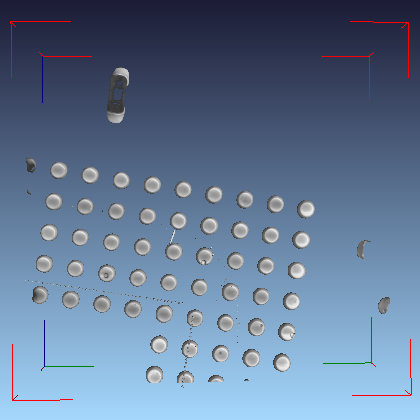
\includegraphics[width=0.5\textwidth]{3ddata.png}
    \caption{3D-Voxeldatensatz in myVGL}
    \label{fig:3ddata1}
  \end{center}
\end{figure}

\item \textbf{2D-Slices} \\
Die zweidimensionalen Slices werden auf Basis der 3D-Voxeldaten berechnet. Dabei wird eine Schicht des Voxelgitters extrahiert und auf Basis der Opazitätswerte eine Rastergrafik erstellt, wobei jeder Pixel eindeutig einem Voxel zugeordnet werden kann. Durch diese Umformung können bei der Objekterkennung auch 2D-Verfahren genutzt werden.

\begin{figure}[H]
  \begin{center}
    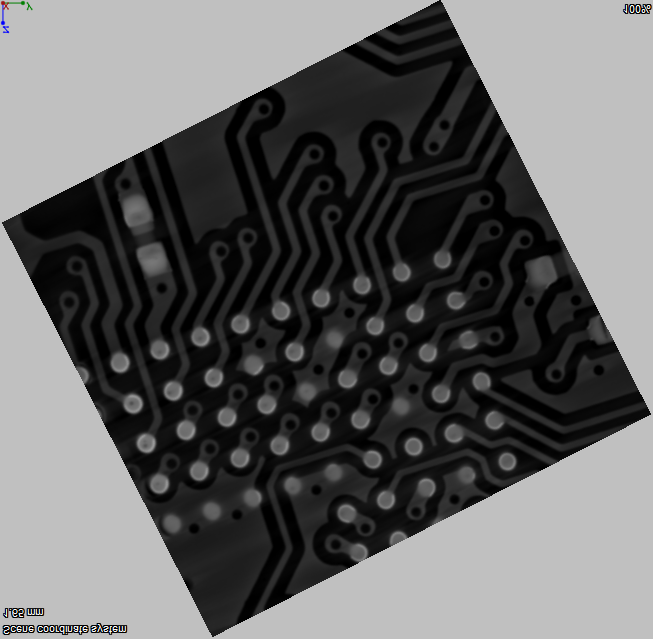
\includegraphics[width=0.5\textwidth]{2ddata.png}
    \caption{2D-Voxeldatensatz}
    \label{fig:3ddata1}
  \end{center}
\end{figure}

\end{enumerate}

%Folgende Zeile aktivieren und als SVN property "svn:keywords" auf "Id" setzen, um SVN Versionsinformationen im Dokument zu erhalten
%\svnInfo $Id: einleitung.tex 60 2012-01-26 15:56:06Z koppor $ 

\chapter{Allgemeine Verfahren}
\label{chap:k3}
	Blablalba
	\subsection {Canny-Edge-Detektor}
		Der Canny-Edge Operator is ein von John Canny 1986 entwickelter Algorithmus zur Kantendetektion. Er liefert für ein Grauwertbild möglichst alle zusammenhängenden Kanten. Der Algorithmus gliedert sich dabei im Wesentlichen in zwei Schritte:
\begin{enumerate}
	\item Kantenhervorhebung
	\item Erzeugung von Katenzügen
\end{enumerate}

Zunächst wird das Bild mit einem zweidimensionalen Gaußkern $G$ gefaltet:
{\[\large \begin{bmatrix}
1 & 2 & 1\\ 
2 & 4 & 2 \\ 
1 & 2 & 1
\end{bmatrix}\]}
Dieser sorgt dafür, dass gröbere Störungen und Rauschen beseitigt werden.
Das gefilterte Bild wird nun auf Kanten hin untersucht. Während Flächen und Segmente in Bildern meist homogene Grauwerte besitzen, stellen Kanten große Grauwertsprünge dar. Um diese Grauwertsprünge zu detektieren, verwendet man den Sobeloperator, ein Filter, der die partiellen Ableitungen eines Pixels in $x$- und $y$-Richtung liefert. \\
Die Struktur eines 1D Sobelfilters ergibt sich dabei aus der finiten Differenz (hier: Zentraldifferenz) an der Stelle $x$:
%\begin{figure}
% 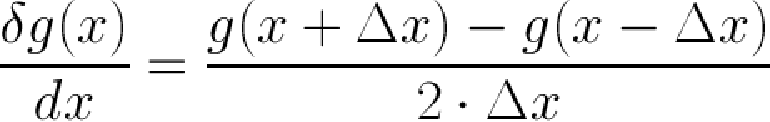
\includegraphics[width=.5\textwidth]{form1.pdf}
%\end{figure}
\begin{equation*}
\frac{\delta g(x)}{dx} = \frac{g(x + \Delta x) - g(x - \Delta x)}{2 \cdot \Delta x }
\end{equation*}
wobei $\Delta x = 1$. Damit hat der diskrete 1D Filter $S$ die Struktur
\begin{equation*}
S = \begin{bmatrix}
1 & 0 & -1
\end{bmatrix}
\end{equation*}
Erweitert auf einen zweidimensionalen Filter ergibt sich

\begin{equation*}
S(x) = \begin{bmatrix}
1 & 0 & -1\\ 
2 & 0 & -2\\ 
1 & 0 & -1
\end{bmatrix},
S(y) = \begin{bmatrix}
1 & 2 & 1\\ 
0 & 0 & 0\\ 
-1 &-2  &-1 
\end{bmatrix}
\end{equation*}

in $x$-, bzw. $y$-Richtung. \\
Die Anwendung der Filter auf das Ausgangsbild liefert die partiellen Ableitungen $G_x$ und $G_y$.
Aus diesen partiellen Ableitungen, die die Anwendung der beiden Filter liefert, lässt sich die Gradientenrichtung $d$ einer Kante berechnen:
\begin{equation*}
d(x, y) = arctan(\frac{G_y(x, y)}{G_x(x, y)})
\end{equation*}
Anschließend wird aus den partiellen Ableitungen ein Bild der absoluten Kantenstärke berechnet:
\begin{equation*}
G(x, y) = \sqrt{G_x(x, y)^2 + G_y(x, y)^2}
\end{equation*}
Im nächsten Schritt wird eine Technik names “Non-maximum suppression” angewandt, um sicherzustellen, dass Kanten nicht breiter als ein Pixel sind. Dabei werden für jedes Pixel seine 8 Nachbarn untersucht. Befindet sich in der Nachbarschaft des zu untersuchenden Pixels ein Pixel, dass einen höheren Grauwert aufweist, so wird der Grauwert des zu untersuchenden Pixels auf 0 gesetzt, es sei denn, das Pixel mit dem größeren Grauwert befindet sich entlang der Gradientenrichtung. \\ \\
Im letzten Schritt des Verfahrens werden die Pixel zu Kantenzügen zusammengefasst.
Dabei verwendet man zwei Schwellwerte $L_1 < L_2$. Zunächst wird nach einem Pixel gesucht, dessen Grauwert größer als $L_2$ ist. Dieses Pixel wird zum Startpixel des Kantenzugs erklärt. Nun wird die Kante in beiden Richtungen nach Pixel mit einem Grauwert größer $L_1$ abgesucht, welche dem Kantenzug hinzugefügt werden. Werden keine Pixel gefunden, die diese Bedingung erfüllen, bricht die Suche ab, und des wird ein neues Startpixel gesucht.Das Verfahren endet, sobald kein unmarkiertes Pixel mit einem Grauwert größer $L_2$ gefunden wird. \\ \\
Als Resultat des Verfahrens entsteht ein Bild, das eine Menge von Pixeln enthält, die idealerweise genau die Kantenpixel des Ausgangsbilds enthält.
\begin{figure}[H]
  \begin{center}
    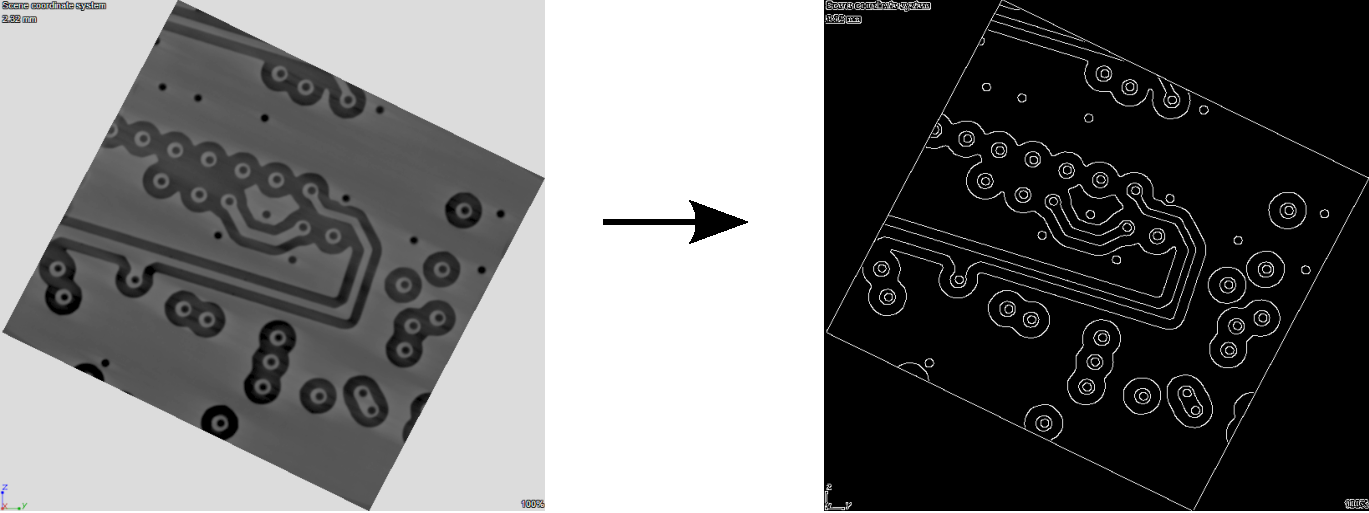
\includegraphics[width=\textwidth]{canny.pdf}
    \caption{Resultat nach der Anwendung des Canny-Edge-Detektors}
    \label{fig:canny}
  \end{center}
\end{figure}


	\subsection {Floodfill-Algorithmus}
Der Floodfill-Algorithmus ist bla..
	\subsection {Houghtransformation}
		\subsubsection{Houghtransformation zur Erkennung von Geraden}
		\subsubsection{Houghtransformation Erkennung von Kreisen}

	

%\vspace{-3cm}
%\vspace{2cm}




%Folgende Zeile aktivieren und als SVN property "svn:keywords" auf "Id" setzen, um SVN Versionsinformationen im Dokument zu erhalten
%\svnInfo $Id: einleitung.tex 60 2012-01-26 15:56:06Z koppor $ 

\chapter{Selektion gut detektierbarer Bilder}
\label{chap:slk}
	Um aus dem beschriebenen Bilderstack möglichst gut detektierbare Einzelbilder zu erhalten, werden hier verschiedene Verfahren vorgestellt, die eine weitgehend automatische Auswahl von Bildern erstellt, die für die weitere Objekterkennung gut geeignet sind. \\
Da der gescannte Mikrochip aus vier Leiterbahnschichten besteht, muss der beim Scannen entstehende Bilderstack in vier Intervalle eingeteilt werden, welches jeweils eine Leiterbahnschicht repräsentiert. 
\begin{figure}[H]
  \begin{center}
    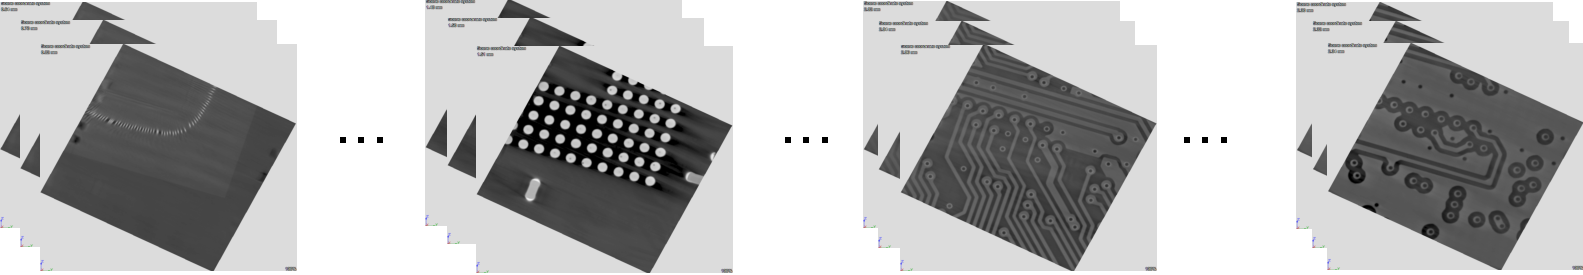
\includegraphics[width=\textwidth]{stack.pdf}
    \caption{Einteilung des Bilderstacks in vier Intervalle}
    \label{fig:intervalls}
  \end{center}
\end{figure}
Ziel der unten vorgestellten Verfahren besteht darin, um für jedes Intervall das Bild zu finden, dass die Leiterbahnschicht am genausten repräsentiert.
Die aus den Verfahren gewonnen Bilder werden anschließend weiterverwendet, d.h. es werden die 2D Objekterkennungsverfahren darauf angewandt und bewertet, wie gut die ausgewählten Bilder für die einzelnen Verfahren geeignet sind, und ob für jedes Intervall tatsächlich das am besten detektierbare Bild gefunden wurde.\\ \\

Um die aufgeführten Verfahren miteinander vergleichen zu können, wird für jedes Intervall das "Best Match" vor dem Vergleich ausgewählt. Dabei handelt es sich um jenes Bild, in dem die Objekte am besten sichtbar sind. Für die vier Intervalle sind dies folgende Bilder:

\begin{figure}[H]
  \begin{center}
    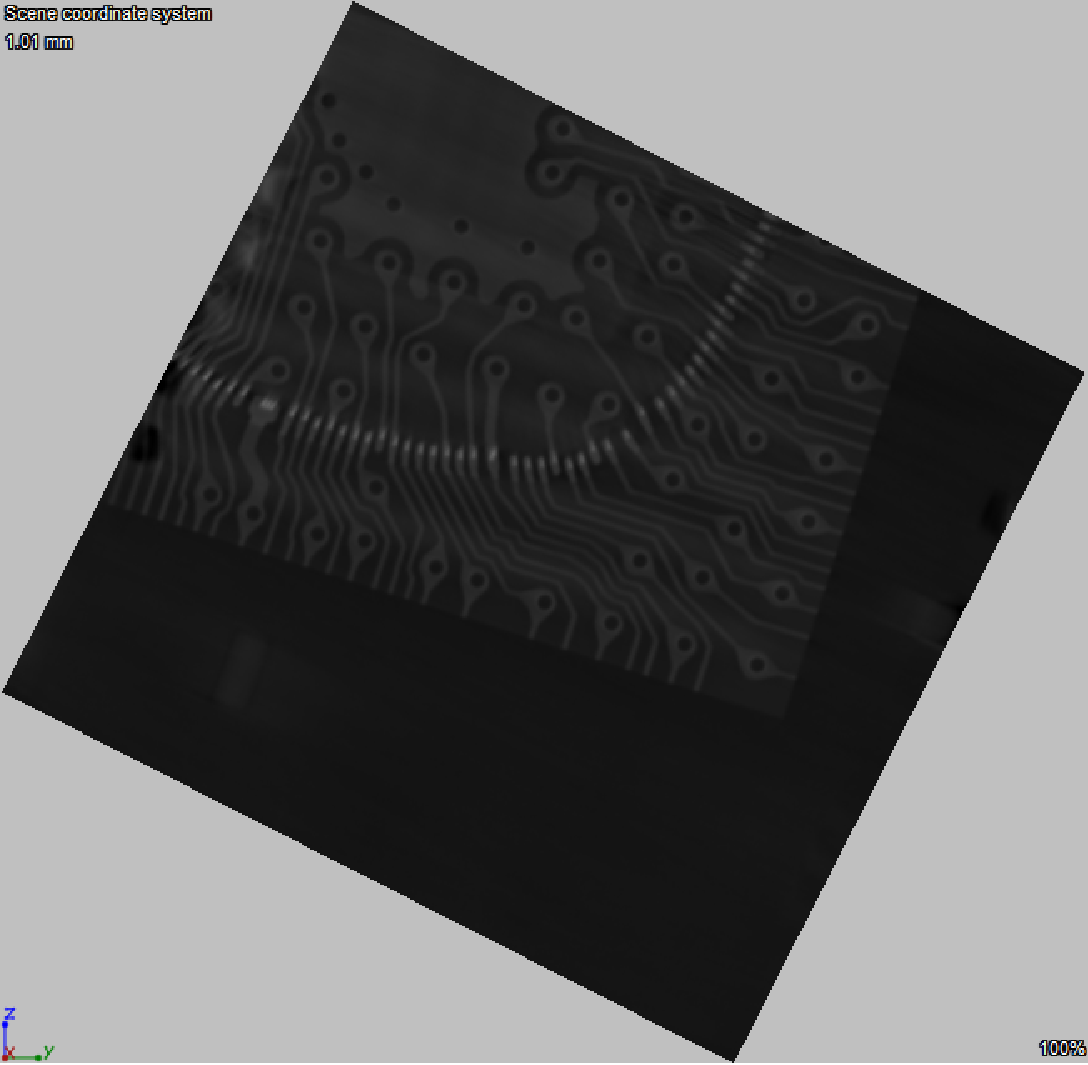
\includegraphics[width=0.5\textwidth]{best1.pdf}
    \caption{Best Match des ersten Intervalls}
    \label{fig:bestmatch1}
  \end{center}
\end{figure}

\begin{figure}[H]
  \begin{center}
    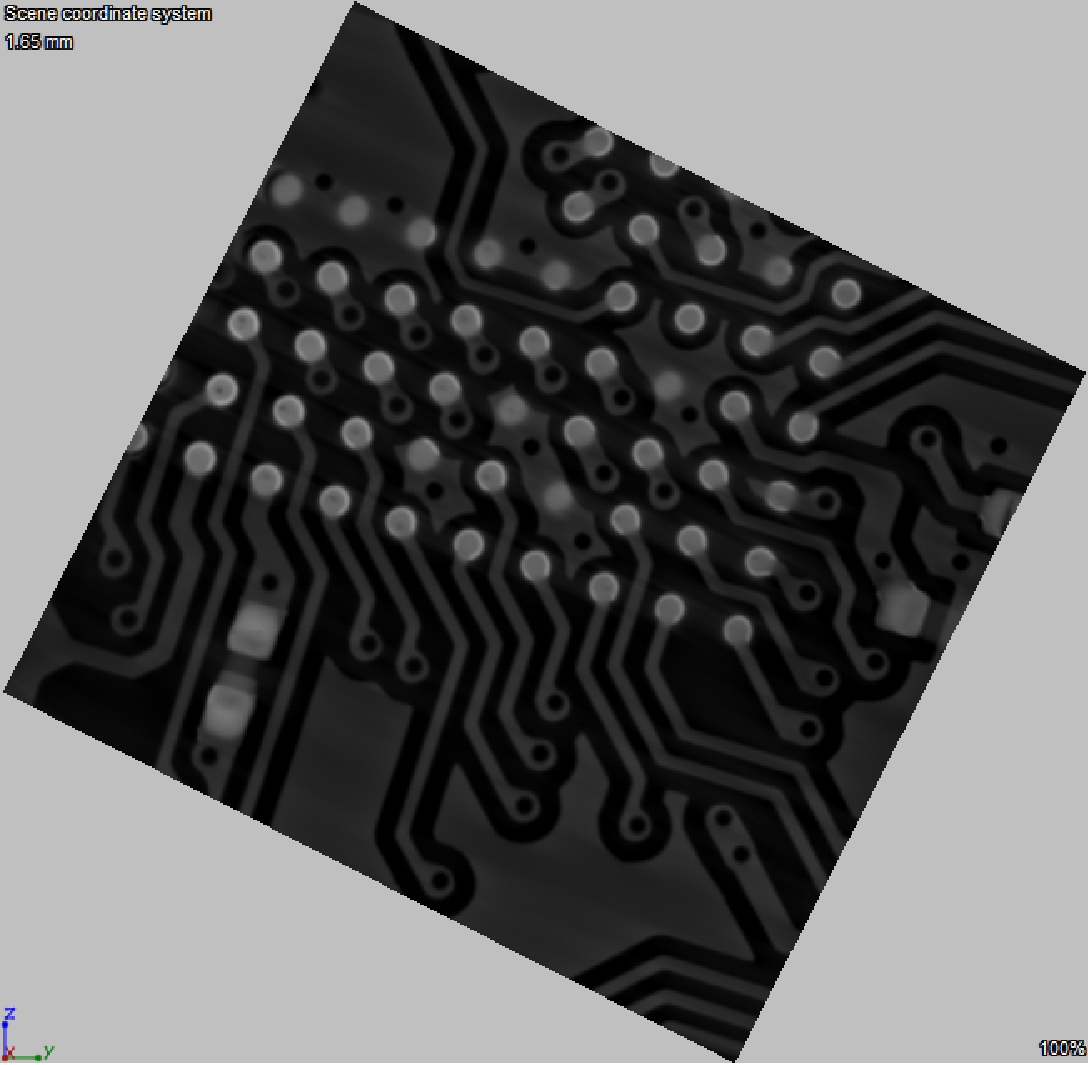
\includegraphics[width=0.5\textwidth]{best2.pdf}
    \caption{Best Match des zweiten Intervalls}
    \label{fig:bestmatch2}
  \end{center}
\end{figure}

\begin{figure}[H]
  \begin{center}
    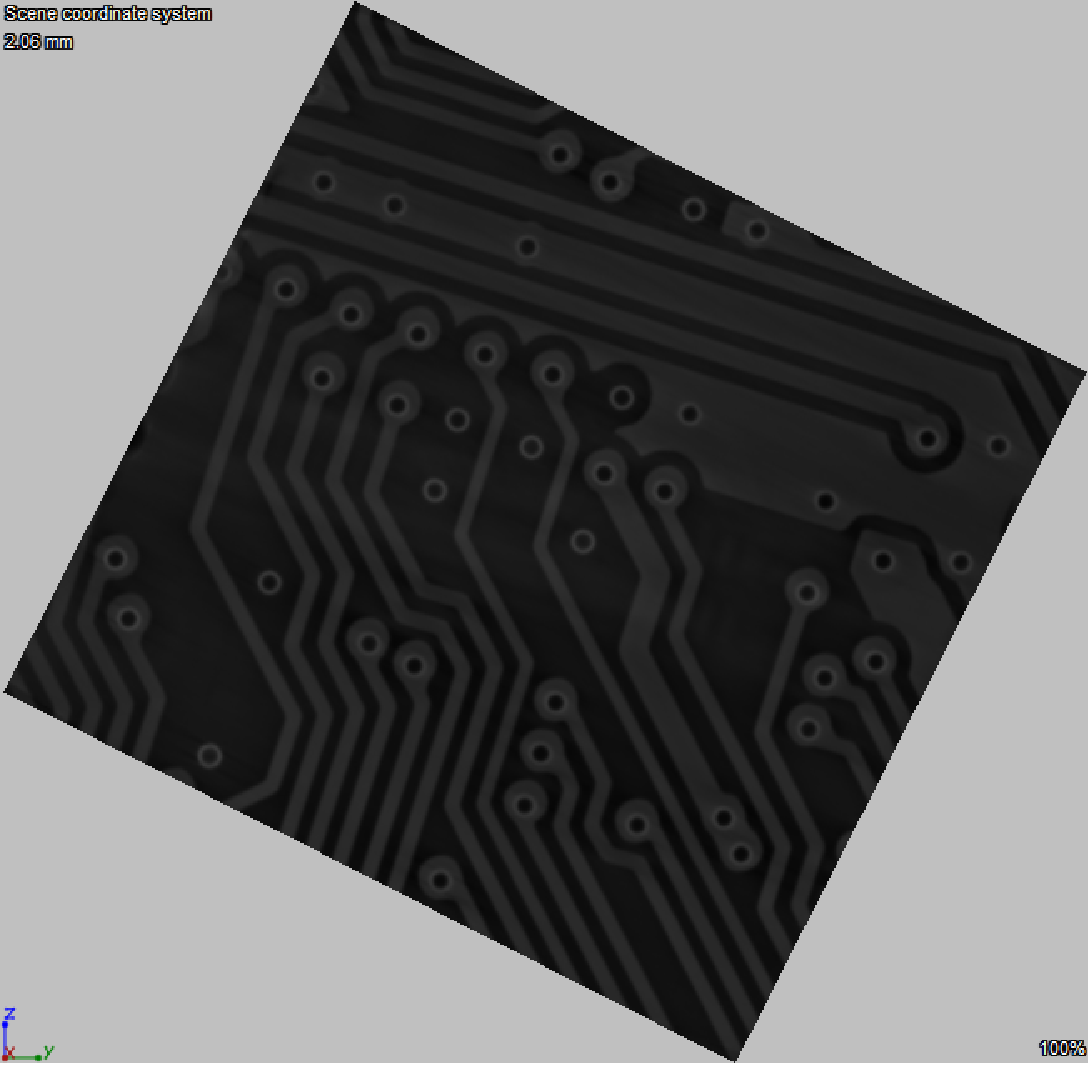
\includegraphics[width=0.5\textwidth]{best3.pdf}
    \caption{Best Match des dritten Intervalls}
    \label{fig:bestmatch3}
  \end{center}
\end{figure}

\begin{figure}[H]
  \begin{center}
    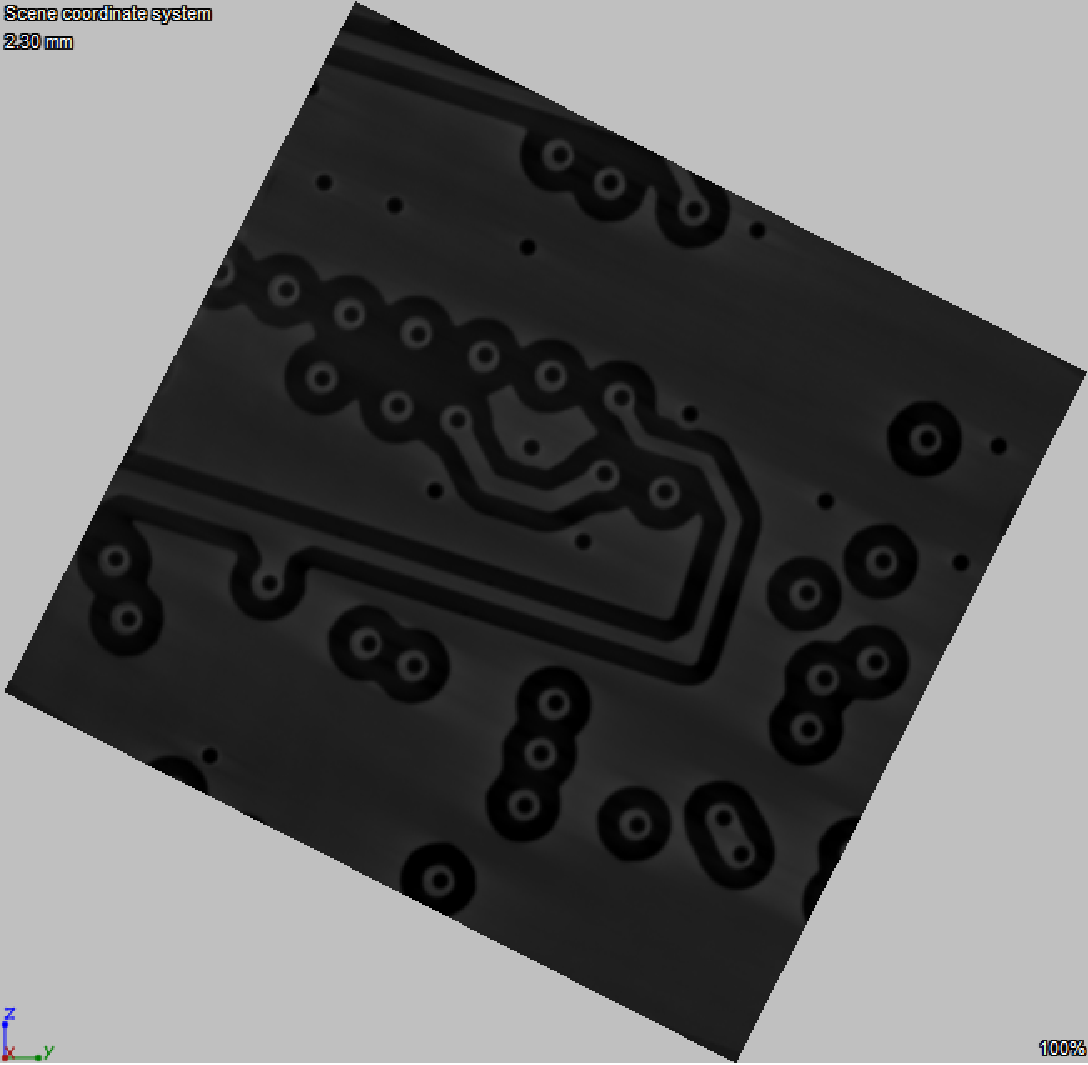
\includegraphics[width=0.5\textwidth]{best4.pdf}
    \caption{Best Match des vierten Intervalls}
    \label{fig:bestmatch4}
  \end{center}
\end{figure}

Diese Best Matches haben im Bilderstack jeweils die Indizes
\begin{enumerate}
	\item{Intervall 1: $Index 27$}
	\item{Intervall 2: $Index 61$}
	\item{Intervall 3: $Index 83$}
	\item{Intervall 4: $Index 96$}
\end{enumerate}

Die Ergebnisse der einzelnen Verfahren werden mit diesen Best Matches verglichen, indem die durschnittliche Distanz der Ergebnisse zu den Best Matches im Bilderstack ermittelt wird. 

\section{Binärbilder}
Bei diesem Verfahren werden zunächst alle Bilder in Binärbilder umgewandelt. Als binärer Schwellwert wird dabei der Wert 70 gewählt, d.h. alle Pixel, deren Grauwert größer als 70 ist, wird der Grauwert 255 zugewiesen, allen Pixeln die einen Grauwert kleiner, bzw. gleich 70 besitzen, wird der Grauwert 0 zugewiesen. Anschließend wird das Bild ausgewählt, welches die maximale Anzahl an weißen Pixeln (Pixel mit dem Grauwert 255) besitzen.

Die Idee, die hinter diesem Verfahren steckt ist, dass Bilder, die eine möglichst große Anzahl von Pixeln mit maximalen Grauwert besitzen, viele Objekte enthalten, die detektiert werden können. \\

\subsection{Ergebnis} 

Die Ergebnisse des Verfahrens für die vier Intervalle:
\begin{figure}[H]
  \begin{center}
    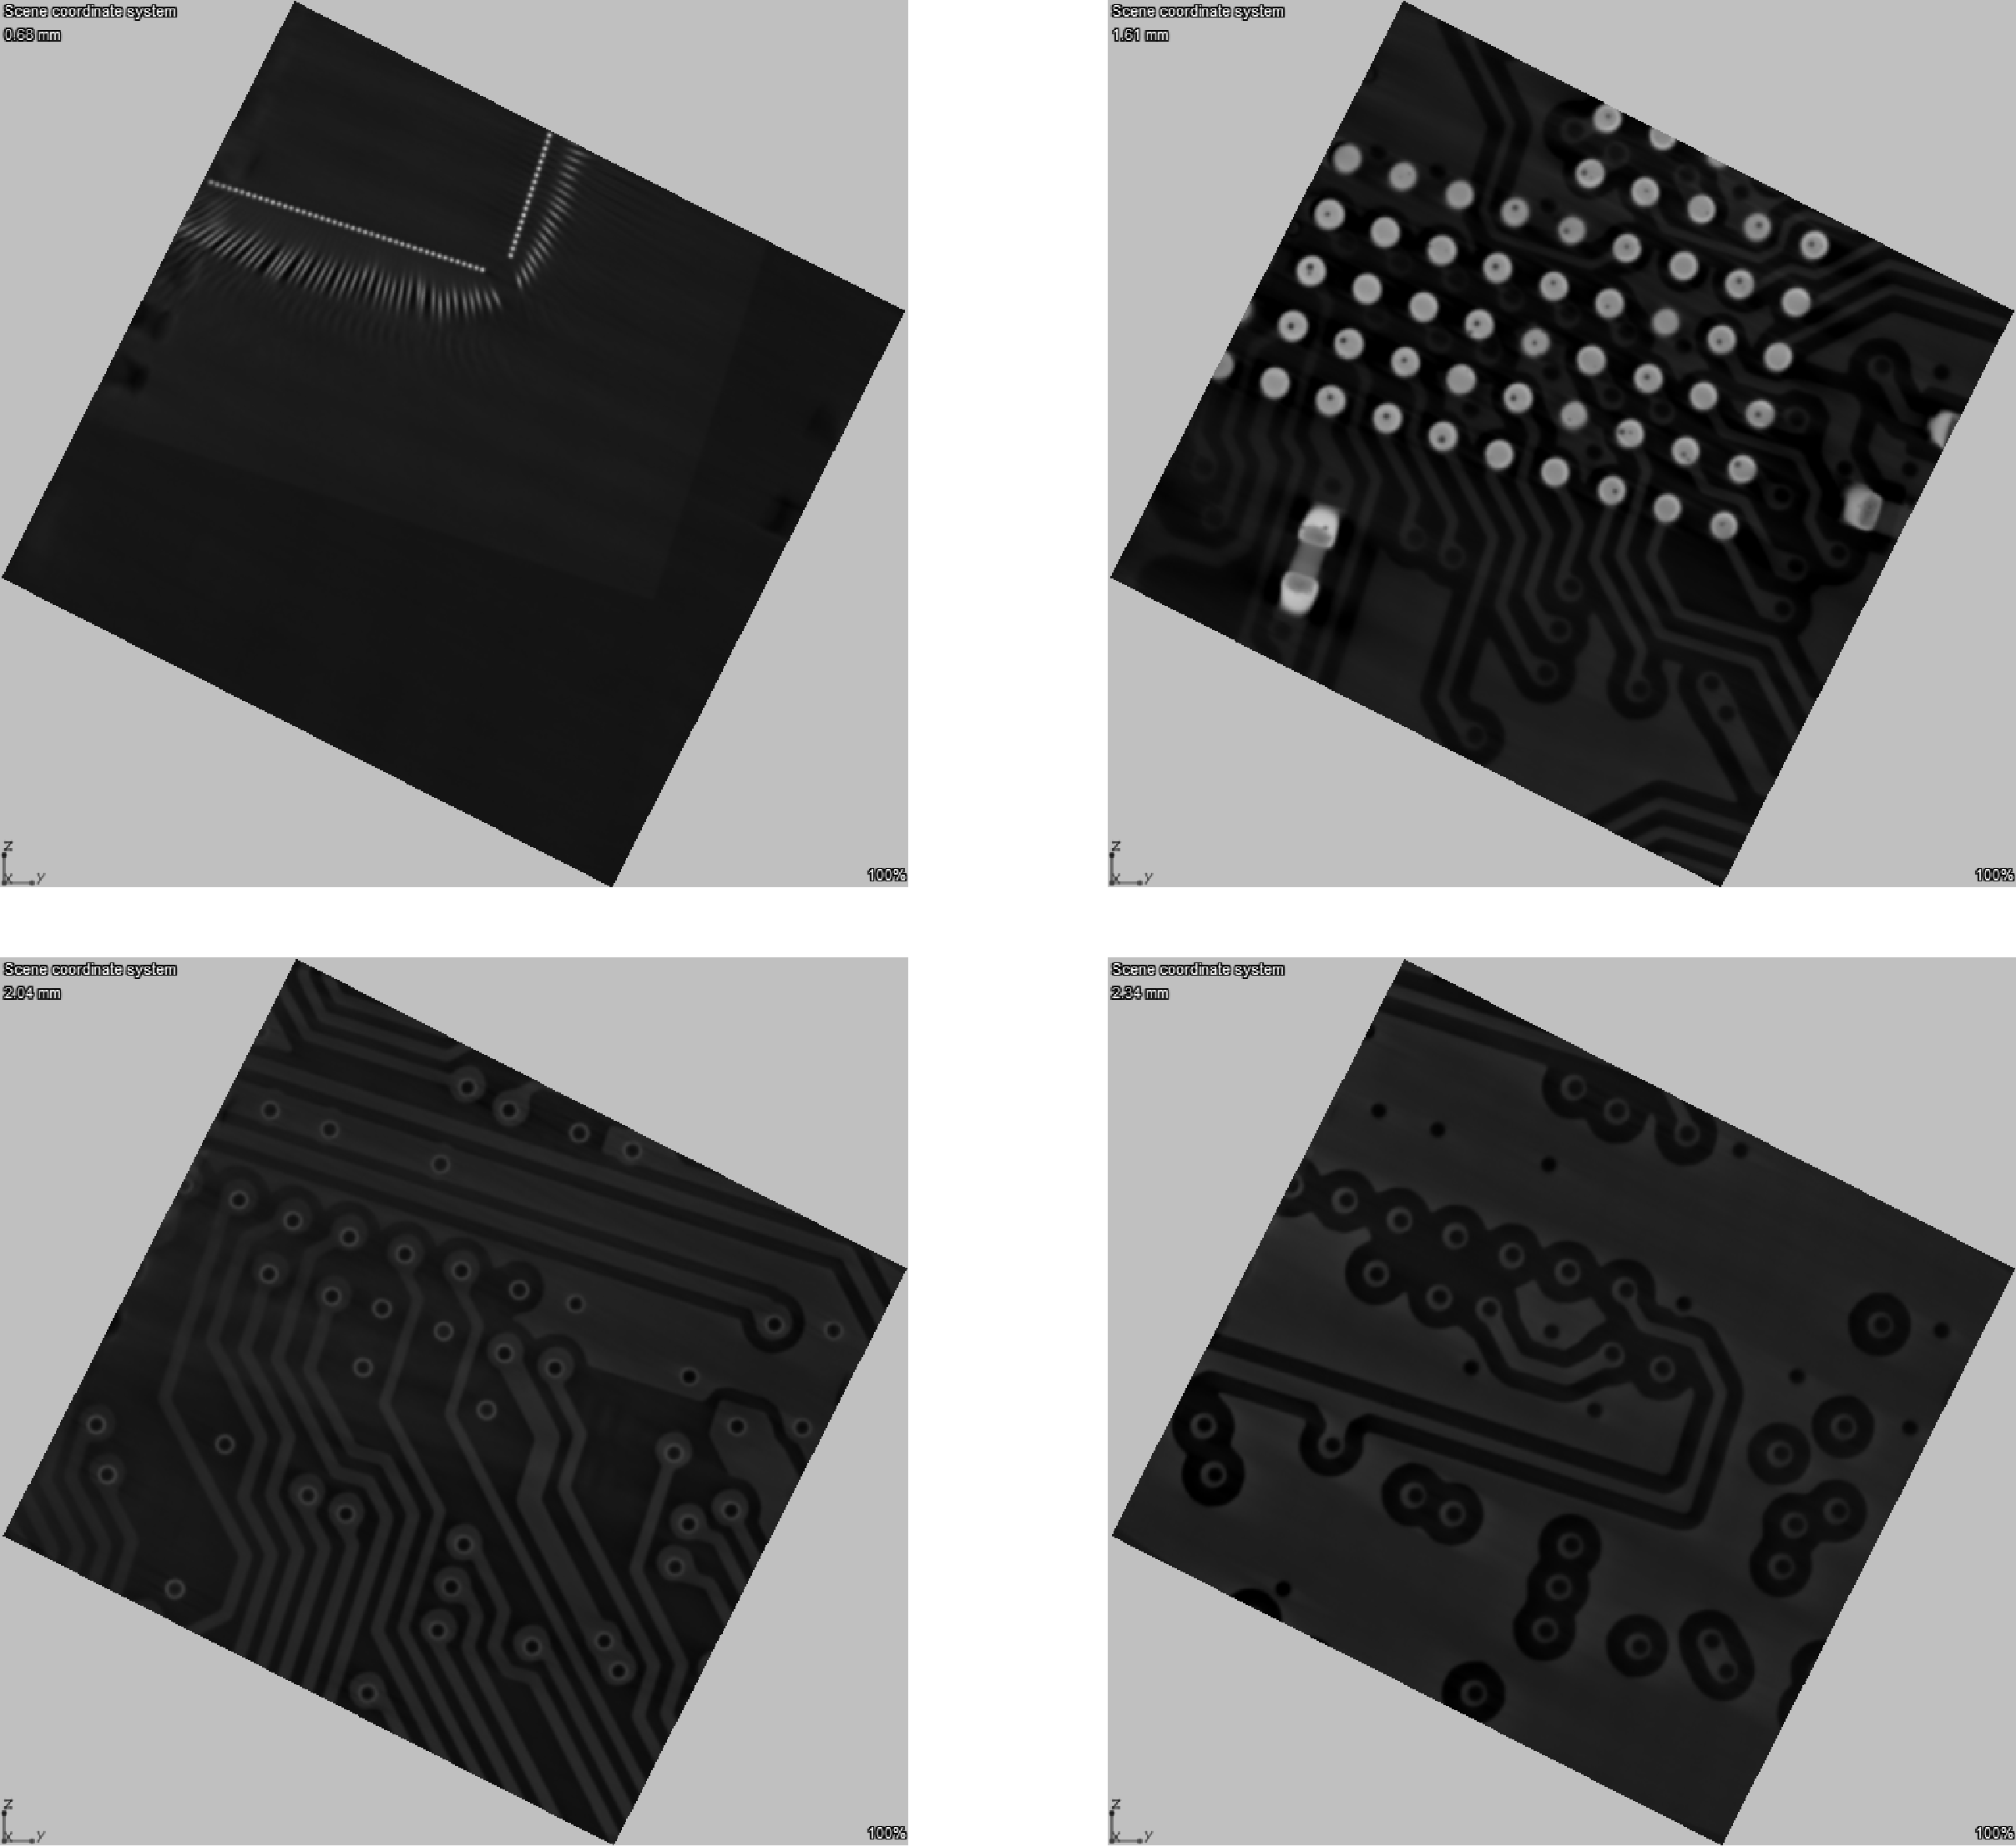
\includegraphics[width=0.9\textwidth]{binary_max.pdf}
    \caption{Ergebnisse des Binärbildverfahrens}
    \label{fig:binary_bestmatch4}
  \end{center}
\end{figure}

Für die einzelnen Intervalle  sind dies die Bilder mit folgenden Indizes:
\begin{enumerate}
	\item{Interval l1: $Index$ $9$ , Differenz zum Best Match: 18}
	\item{Intervall 2: $Index$ $59$, Differenz zum Best Match: 2}
	\item{Intervall 3: $Index$ $82$, Differenz zum Best Match: 1 }
	\item{Intervall 4: $Index$ $98$, Differenz zum Best Match: 2}
\end{enumerate}

Dies führt zu einer durchschnittlichen Distanz von \textbf{5,75} vom Best Match.


\section{Canny-Edge-Bilder}
Bei diesem Verfahren werden die einzelnen Bilder der Intervalle zunächst mit dem Canny-Edge Operator in die entsprechenden Kantenbilder überführt. Anschließend werden die Kantenpixeln in den Kantenbildern gezählt, wobei für jedes Intervall das Bild ausgewählt wird, dass die meisten Kantenpixel besitzt.\\

Der Ansatz hierbei ist, dass Bilder, die viele einzelne Objekte enthalten, mehr Kantenpixel liefern, als Bilder, in denen wenige Objekte enthalten sind.

\subsection{Ergebnis} 

Die Ergebnisse des Verfahrens für die vier Intervalle:
\begin{figure}[H]
  \begin{center}
    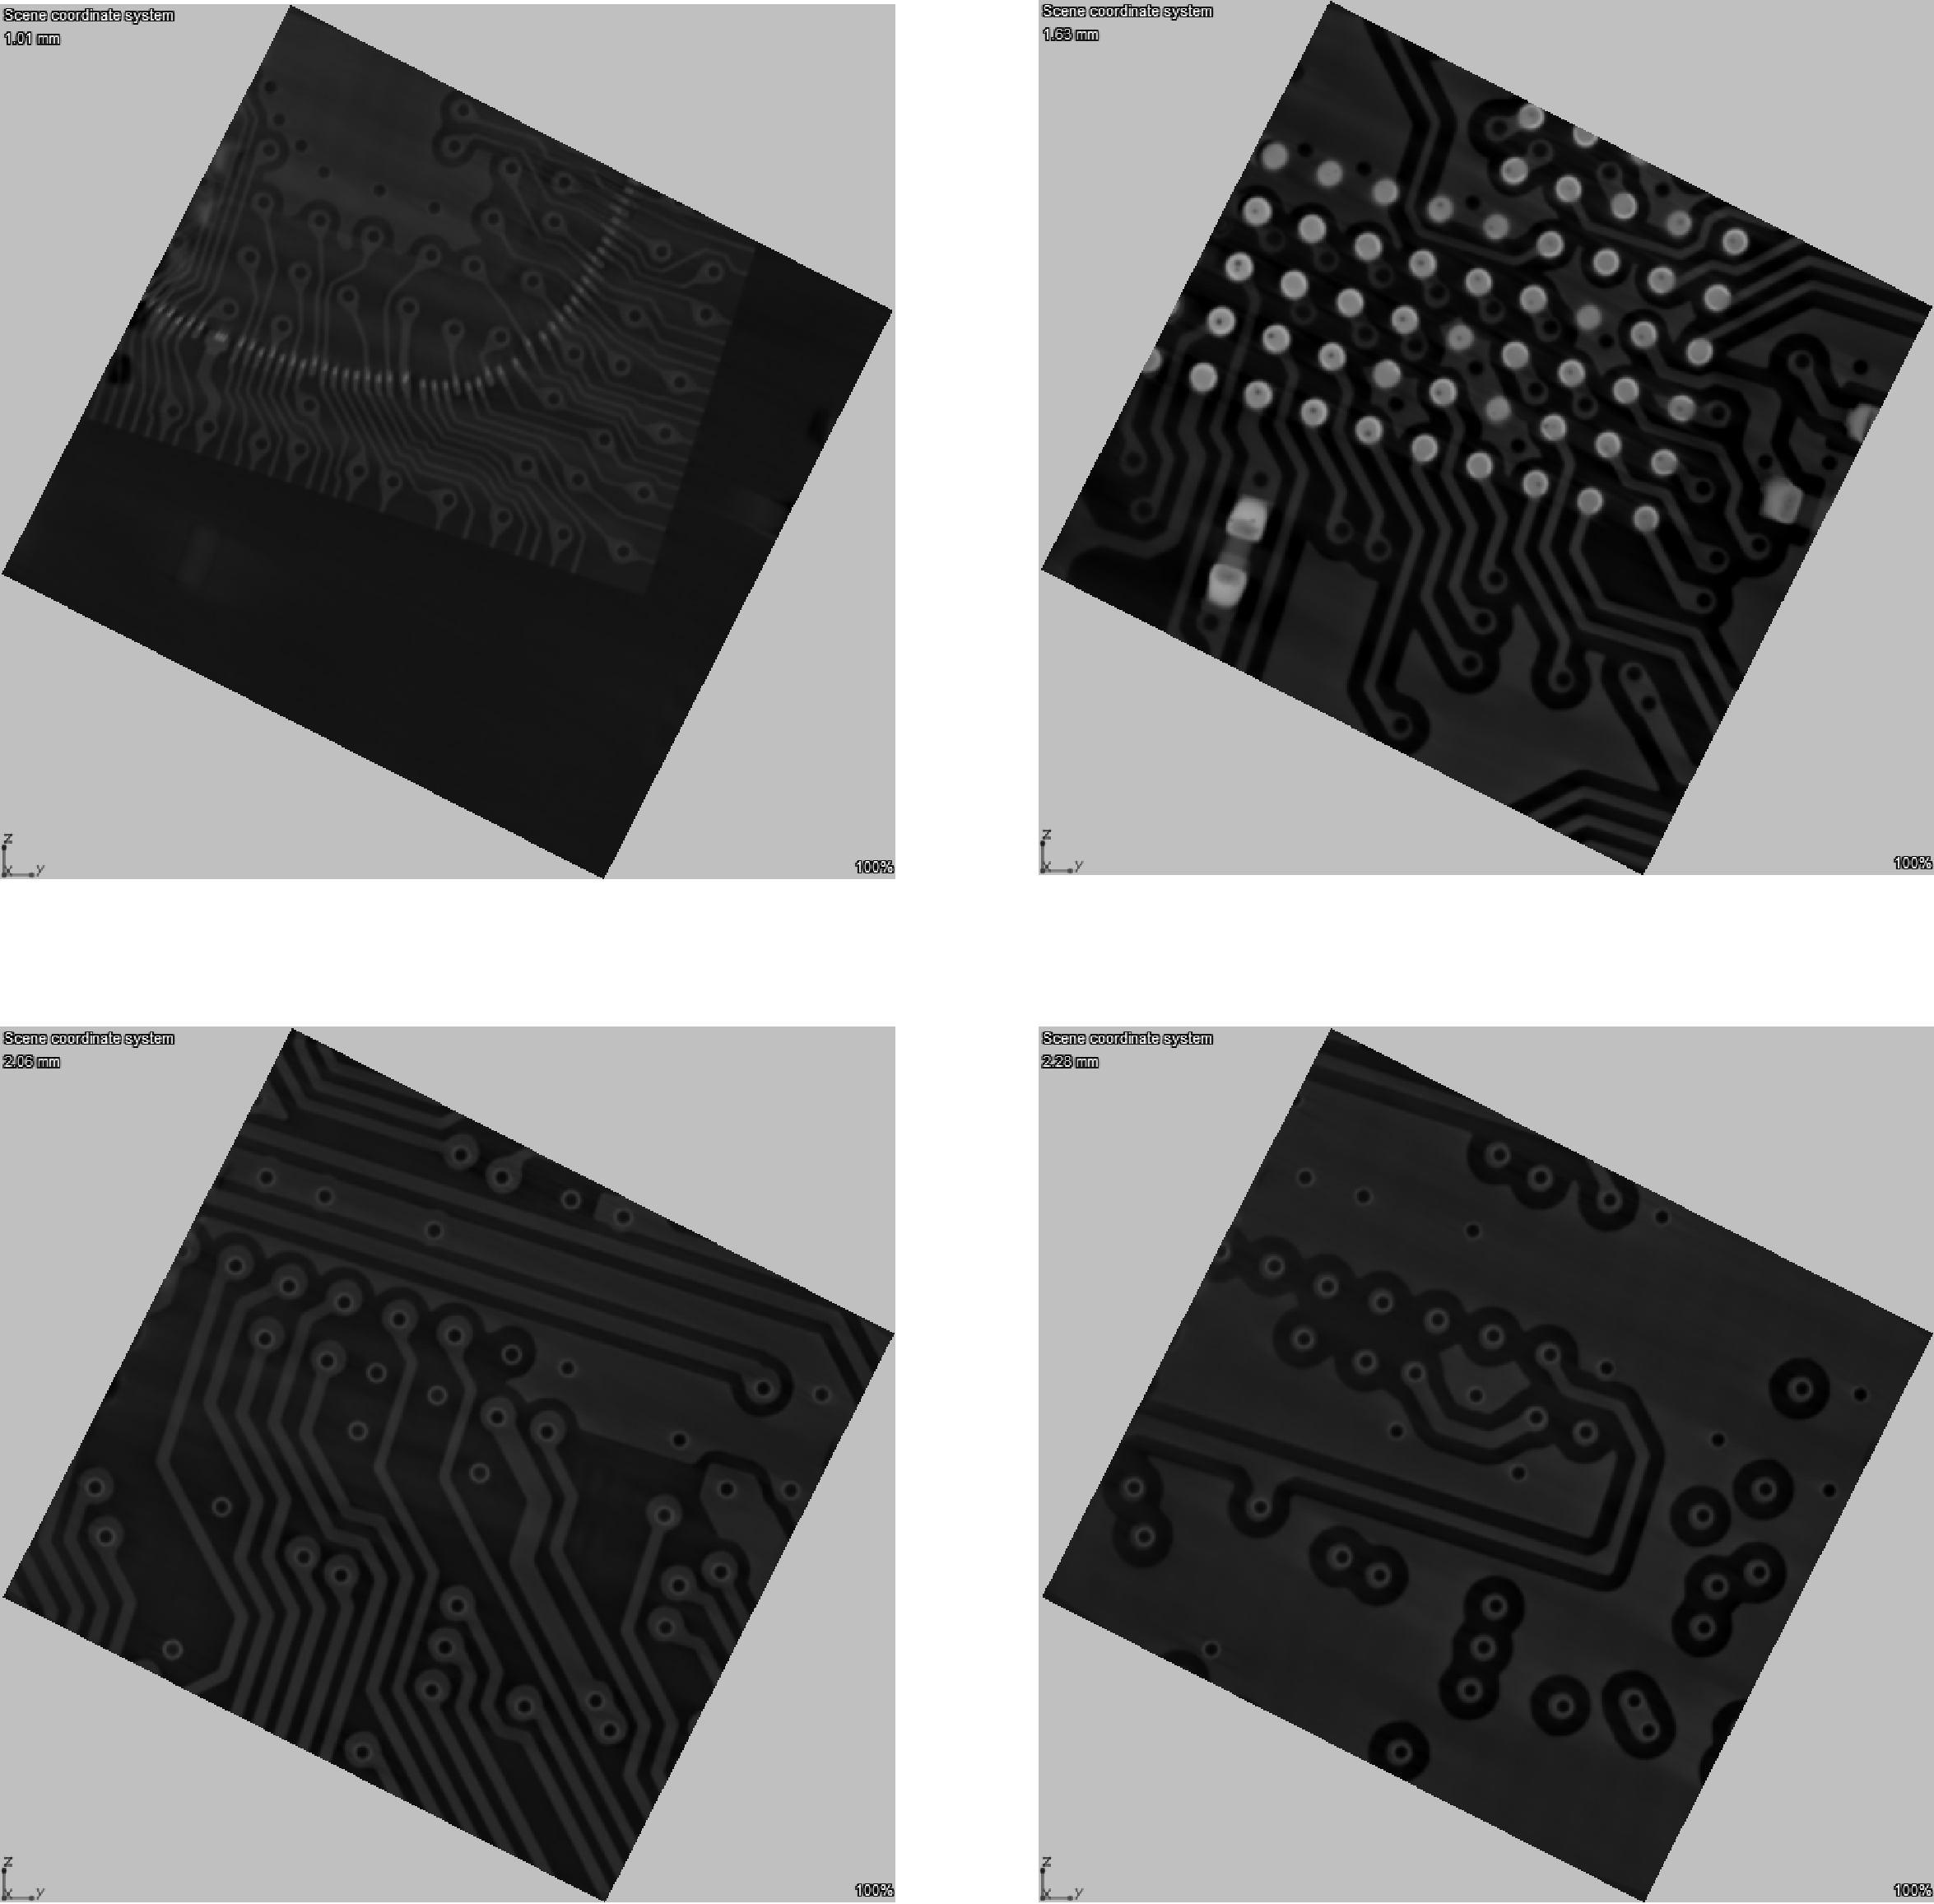
\includegraphics[width=0.9\textwidth]{canny_max_results.pdf}
    \caption{Ergebnisse des Canny-Edge-Verfahrens}
    \label{fig:canny_bestmatch4}
  \end{center}
\end{figure}

Die zugehörigen Katenbilder:
\begin{figure}[H]
  \begin{center}
    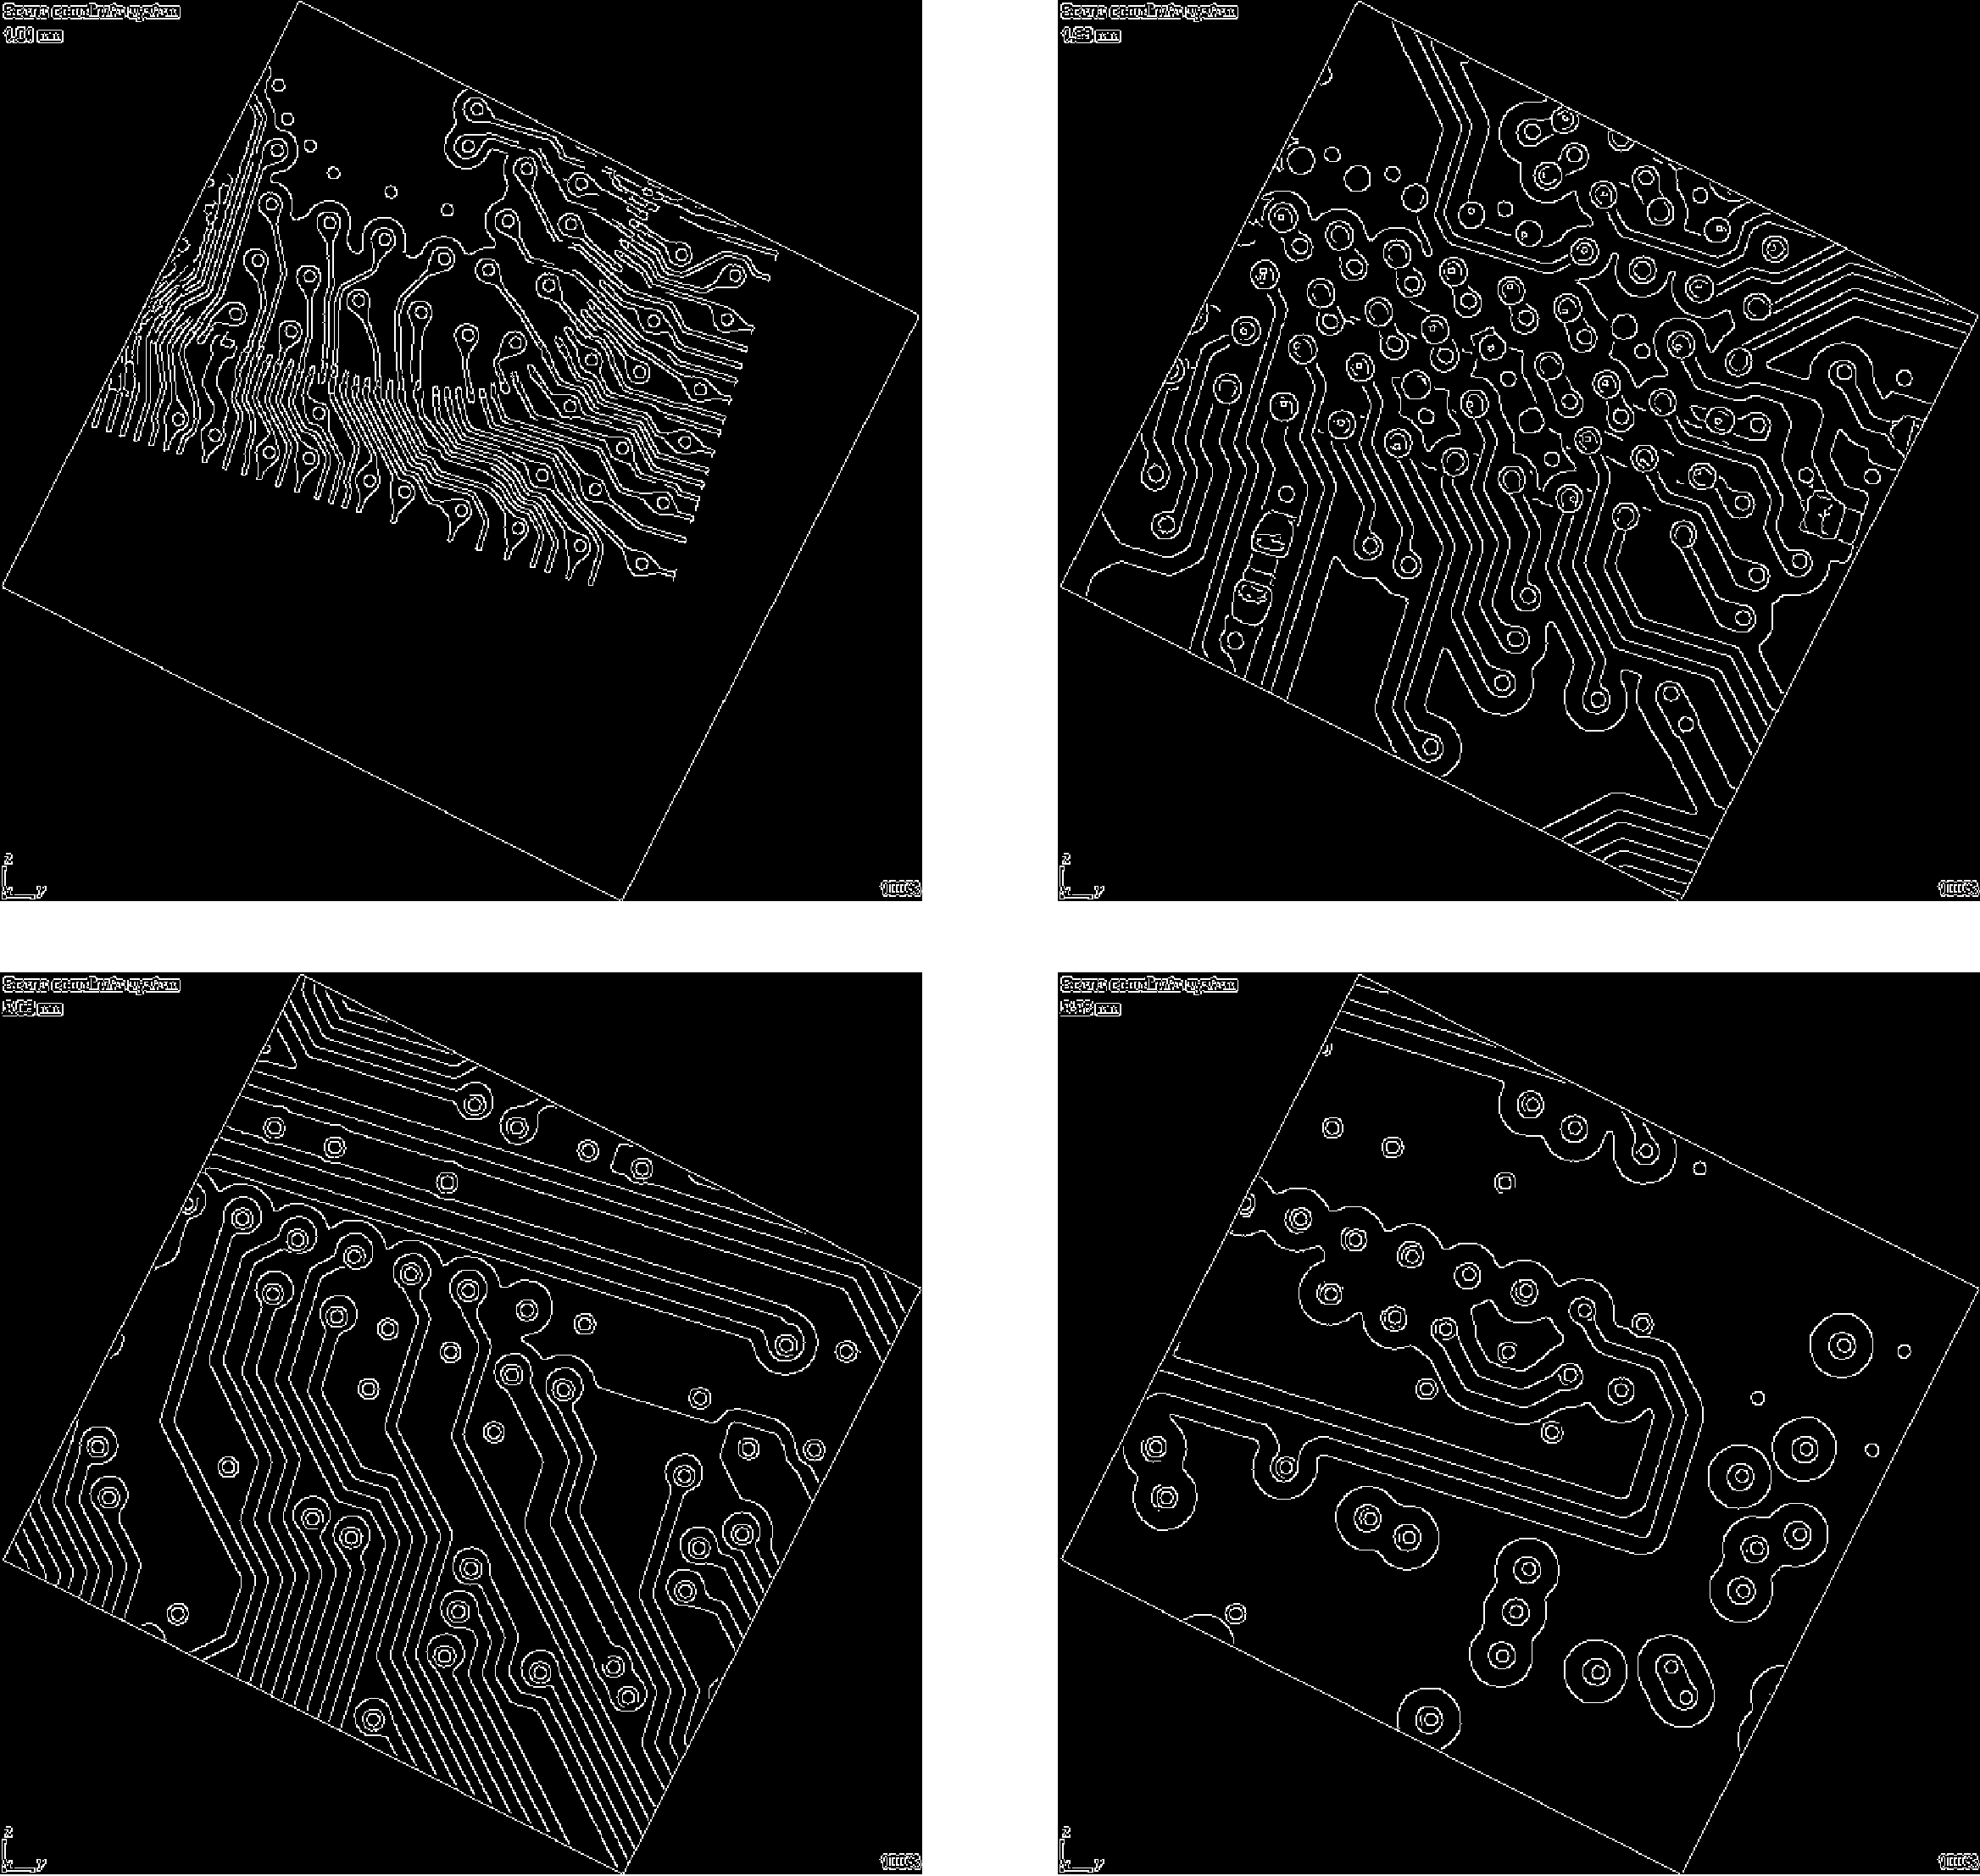
\includegraphics[width=0.9\textwidth]{canny_max_canny_results.pdf}
    \caption{Kantenbilder der Ergebnisse des Canny-Edge-Verfahrens}
    \label{fig:canny_max_bestmatch4}
  \end{center}
\end{figure}

Für die einzelnen Intervalle sind dies die Bilder mit folgenden Indizes:
\begin{enumerate}
	\item{Intervall 1: $Index$ $27$, Differenz zum Best Match: 0}
	\item{Intervall 2: $Index$ $60$, Differenz zum Best Match: 1}
	\item{Intervall 3: $Index$ $83$, Differenz zum Best Match: 0}
	\item{Intervall 4: $Index$ $95$, Differenz zum Best Match: 1}
\end{enumerate}

Dies führt zu einer durchschnittlichen Distanz von \textbf{0,5} vom Best Match.


\section{Hough-Transformation}
Dieses Verfahren ziehlt darauf ab, die Bilder in den Intervallen zu finden, die möglichst gut detektierbare Kantenverläufe, und somit möglichst gut erkennbare Leiterbahnen enthalten. \\
Dafür werden aus den Bildern mit Hilfe der Houghtransformation die Kanten extrahiert und anschließend gezählt. Das Maximum für jedes Intervall ist jenes Bild, welches die meisten zählbaren Kanten enthält.

\subsection{Ergebnis} 

Die Ergebnisse des Verfahrens für die vier Intervalle:
\begin{figure}[H]
  \begin{center}
    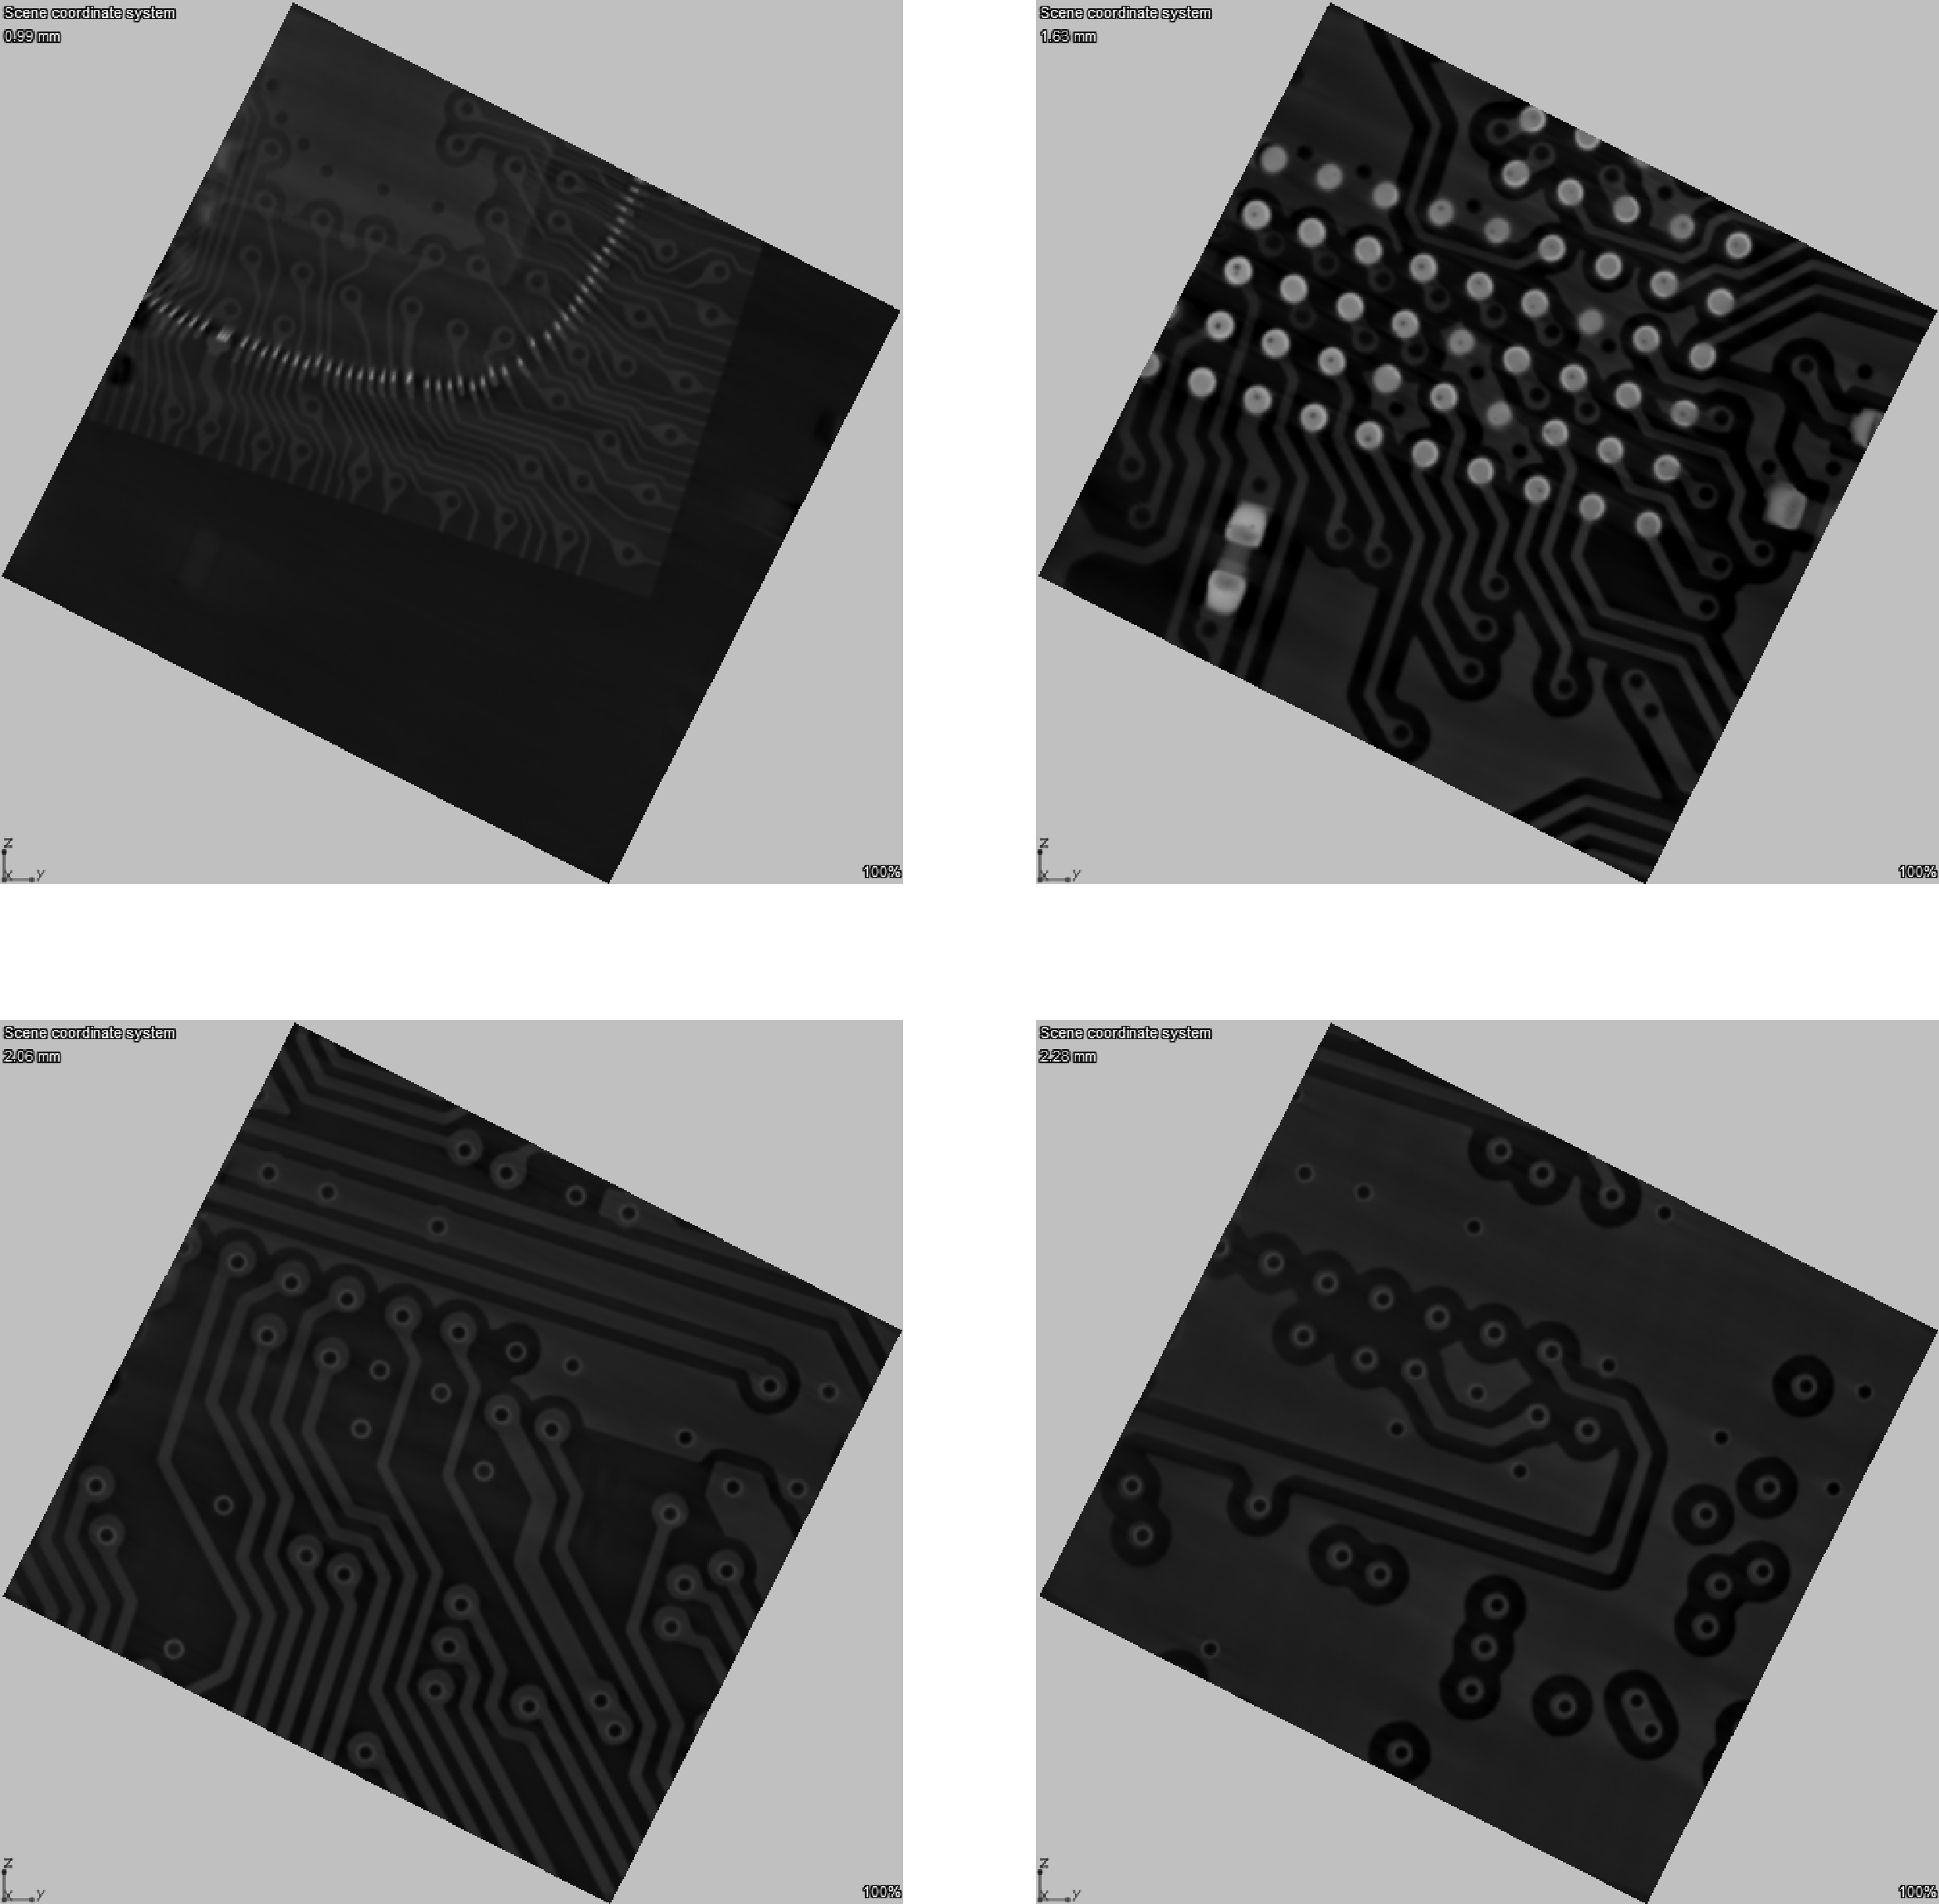
\includegraphics[width=0.9\textwidth]{hough_max.pdf}
    \caption{Ergebnisse des Houghtransformationsverfahrens}
    \label{fig:hough_bestmatch4}
  \end{center}
\end{figure}

Für die einzelnen Intervalle sind dies die Bilder mit folgenden Indizes:
\begin{enumerate}
	\item{Intervall 1: $Index$ $26$, Differenz zum Best Match: 1}
	\item{Intervall 2: $Index$ $60$, Differenz zum Best Match: 1}
	\item{Intervall 3: $Index$ $83$, Differenz zum Best Match: 0}
	\item{Intervall 4: $Index$ $95$, Differenz zum Best Match: 1}
\end{enumerate}

Dies führt zu einer durchschnittlichen Distanz von \textbf{0,75} vom Best Match.

\section{Vergleich}
Es ist deutlich zu erkennen, dass das Binärbildverfahren deutlich schlechtere Ergebnisse (durchschnittliche Distanz: $5,75$) liefert, als das Canny-Edge-Verfahren (durchschnittliche Distanz: $0,5$) und das Houghtransformationsverfahren (durchschnittliche Distanz: $0,75$). Dies liegt vor allem daran, das Störpixel, bzw. für die weitere Verarbeitung irrellevante Informationen in Form von nicht defninierten Objekten einen starken Einfluss auf die Menge der weißen Pixel nehmen. Beim Canny-Edge-Verfahren werden primär "echte" Objekte, also Objekte, die aus zusammenhängenden Kanten bestehen extrahiert, während Störpixel ber der Überführung der Bilder in Kantenbilder gefiltert werden. \\
Ein minimal schlechteres Ergebniss liefert das Houghtransformationsverfahren, da dieses Verfahren eine gute detektierbarkeit der Leiterbahnen berücksichtigt, Bohrpunkte allerdings außer Acht lassen.



%Folgende Zeile aktivieren und als SVN property "svn:keywords" auf "Id" setzen, um SVN Versionsinformationen im Dokument zu erhalten
%\svnInfo $Id: einleitung.tex 60 2012-01-26 15:56:06Z koppor $ 

\chapter{2D - Verfahren}
\label{chap:2d}
	\section{SIFT}
\cite{Lowe2004} \\
		SIFT (Scale-invariant feature transform) ist ein von David Lowe 1999 vorgestelltes Verfahren zur Extraktion von lokalen Merkmalen aus Bildern. Die mit diesem Verfahren gefundene Merkmale haben die Eingeschaft, dass sie robust gegenüber Rotation, Translation und Skalierung sind, und damit zuverlässig in anderen Bilder wiedererkannt werden können. \\
Um Objekte in Bildern mit SIFT erkennen und lokalisieren zu können, sind also zwei Schritte nötig:
\begin{enumerate}
	\item Extraktion und Beschreibung von Merkmalen (Features) des gesuchten Objekts
	\item Lokalisation der Merkmale im Suchbild
\end{enumerate}

\subsection{Extraktion und Beschreibung von Merkmalen (Features) des gesuchten Objekts}
Der Algorithmus zur Extraktion und Beschreibung der Merkmale besteht dabei aus vier Verarbeitungsstufen:
	\subsubsection{Ermittlung potentieller Merkmale in DoG-Pyramiden}
		Um Merkmale zu ermitteln, die robust gegenüber Skalierung sind, kommt das Verfahren der DoG (Difference of gaussians) Pyramiden zum Einsatz. Dabei werden aus dem Ausgangsbild zunächst n Gaußpyramiden berechnet. Eine Pyramide besteht dabei aus fortlaufen stärker geglätteten Bildern des Ausgangsbildes $g$. Zur Glättung kommt dabei ein Gaußfilter $G$ zum Einsatz:
\begin{equation*}
 g(x, y) * G_\vartheta (x, y) = g(x, y) * (\frac{1}{\sqrt{2\pi \vartheta ^2}}\cdot e^{-\frac{x^2 + y^2}{2\vartheta ^2}})
\end{equation*}

Im Anschluss wird das letzte Bild der Pyramide um 50\% verkleinert, und daraus durch erneute fortlaufende Glättung mit dem Gaußfilter eine neue Pyramide erzeugt.
Je zwei benachbarte Bilder einer Gaußpyramide werden nun voneinander Subtrahiert. Aus den Resultaten entstehen dabei die DoG Pyramiden:
\begin{figure}
  \begin{center}
    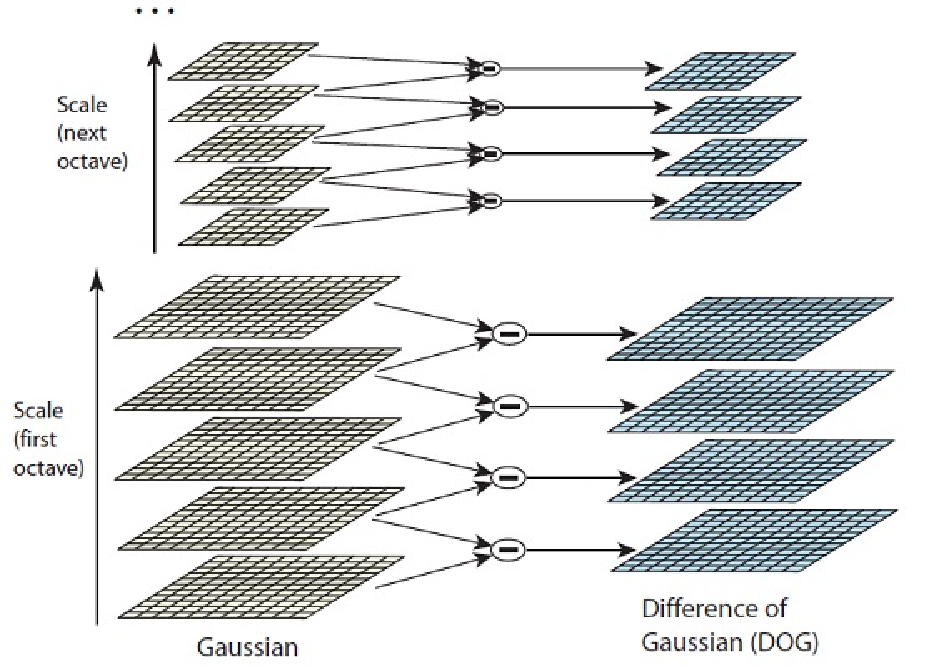
\includegraphics[width=\textwidth]{dog.pdf}
    \caption{DoG-Pyramiden}
    \label{fig:dog_pyr}
  \end{center}
\end{figure}

Die dadurch erzeugten DoG-Pyramiden werden nun auf minimale und maximale Pixelwerte untersucht.
Ein Maximum ist gefunden, wenn der Grauwert eines Pixels größer als der seiner 26 Nachbarn ist. Nachbarschaft eines Pixels ergibt sich dann aus seinen acht Nachbarn der selben Ebene, sowie aus den jeweils neun Nachbarn der benachbarten Ebenen in der DoG-Pyramide.
Die Suche nach Minima erfolg auf die selbe Art und Weise. Die Information, auf welcher Skalierung die potentiellen Merkmalspunkte liegen, wird dabei ebenfalls gespeichert.
\begin{figure}[H]
  \begin{center}
    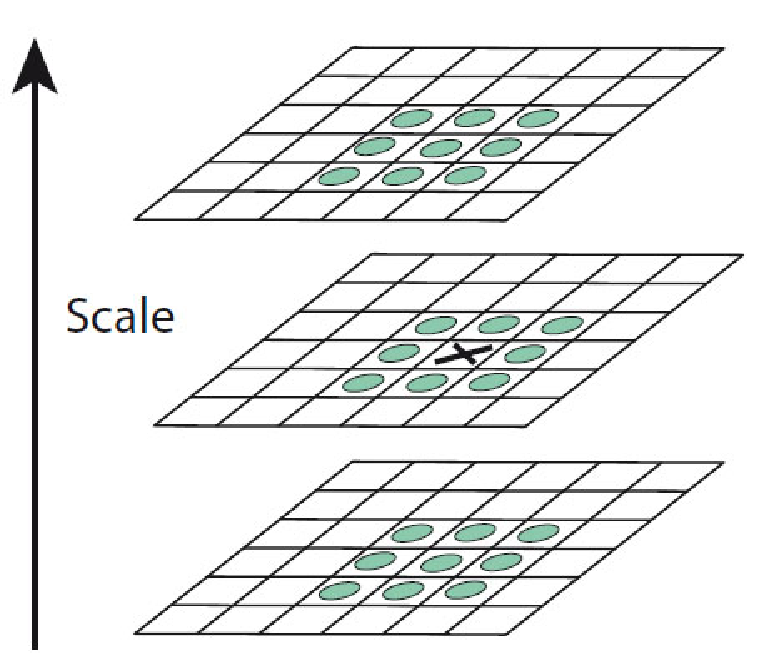
\includegraphics[width=0.5\textwidth]{scale.pdf}
    \caption{Nachbarschaft eines Pixels}
    \label{fig:neighbor}
  \end{center}
\end{figure}
	\subsubsection{Filterung und Lokalisation potentieller Merkmalspunkte}
		Das oben genannte Verfahren liefert neben den robusten Merkmalspunkten eine große Menge von instabilen, für die weitere Verarbeitung nicht zu gebrauchende Merkmale.
Daher werden die gefundenen Merkmalspunkte anhand von Stabilitätskriterien gefiltert.
Im ersten Schritt werden dabei alle Merkmalspunkte entfernt, die einen DoG-Wert von weniger als 0,03, und somit einen relativ niedrigen Kontrast besitzen.
Merkmalspunkte, die auf Ecken liegen sind “prägnanter” (und somit staibler) als solche, die auf einer Kante liegen, daher werden alle Merkmalspunkte entfernt, die auf einer Kante, aber nicht auf einer Ecke liegen.
Dies geschieht unter Anwendung der Hesse-Matrix (todo).
	\subsubsection{Bestimmung der Hauptorientierungen}
		Um Invarianz der verbleibenden Merkmalspunkte gegenüber Rotation zu erreichen, wird für jeden Merkmalspunkt dessen Hauptorientierung berechnet.
Dafür nutzt man das gaußgefilterte Bild, welches der Skalierung des zu untersuchenden Merkmalspunktes am nächsten kommt. In diesem Bild werden nun innerhalb einer festen Region um den Merkmalspunkt herum die Gradientenlängen $m(x, y)$ und die Gradientenorientierungen $\theta (x, y)$ bezüglich eines Punktes $g(x, y)$ berechnet, wobei
\begin{equation*}
m(x, y) = \sqrt{(g(x + 1, y) - g(x - 1, y))^2 +(g(x, y+1) - g(x, y-1))^2}
\end{equation*}

und

\begin{equation*}
\theta (x, y) = tan^{-1}\cdot \frac{g(x +1, y) - g(x-1, y)}{g(x, y +1) - g(x, y-1)}
\end{equation*}

Die so ermittelten Gradientenorientierungen werden nun anhand ihrer Gradientenlängen gewichtet. Dadurch haben Gradientenrichtungen mit großer Gradientenlänge einen größeren Einfluss auf die Hauptorientierung als Gradientenrichtungen mit niedriger Gradientenlänge.
Danach werden die Gradientenorientierungen zusätzlich anhand ihrer Entfernung zum Merkmalspunkt gewichtet, um Gradientenrichtungen, die sich näher am Merkmalspunkt befinden stärker zu gewichten.

Aus den gewichteten Gradientenorientierungen wird nun ein Orientierungshistogramm erstellt. Dieses Histogramm ist in 36 Winkelbereiche eingeteilt und hat somit eine Klassenbreite von $10\,^{\circ}$.
Jede Gradientenorientierung wird dabei anhand ihrer Gewichtung an der passenden Stelle im Histogramm aufaddiert. \\
Nach der Erstellung des Histogramms kann aus diesem die Gradientenlänge $m_{max}$ abgelesen werden (Winkelbereich mit der größten Summe). Die Hauptorientierung des Merkmalspunktes  setzt sich dabei aus $m_{max}$, sowie der zugehörigen Gradientenorientierung $\theta_{max}$ maxzusammen.
Für den Fall, dass eine weitere Orientierung mit der Gradientenlänge $m_i > 0,8 m_{max}$
existiert; wie es bei Eckpunkten häufig der Fall ist; wird an der Stelle $(x, y)$ ein weiterer Merkmalspunkt mit der Hauptorientierung $(m_i, \theta_i)$ erstellt.
\subsection{Lokalisation der Merkmale im Suchbild}
Wurden nun im ersten Schritt die robusten Merkmale des gesuchten Objekts extrahiert, können diese im Suchbild wiedererkannt werden.
Dies geschieht, in dem man die extrahierten Merkmale des Objekts mit denen im Suchbild auf Übereinstimmung hin untersucht. \\
Der dafür am häufigsten verwendete Ansatz ist der vergleich anhand des euklidischen Abstands der Merkmalsvektoren.
\begin{equation*}
e = \sqrt{\sum_{i = 1}^{n}(V_{1i} - V_{2i})}
\end{equation*}

\section{Einsatz von SURF zur Erkennung von Bohrpunkten}
Um in den Beispieldatensätzen Bohrpunkte auf möglichst effiziente Art und Weise erkennen zu können, wird hier SURF ($Speeded Up Robust Features$), eine leicht veränderte Variante des SIFT-Verfahrens, verwendet. \\
Der Unterschied zum hier vorgestellen SUFT Verfahrens besteht darin, dass statt der Gaußfilter Mittelwertfilter zum Einsatz kommen. Dadurch wird das Verfahren signifikant beschleunigt, ohne die Erkennungsrate nennenswert zu beeinflussen. \cite{Bay2005} \\

Um Bohrpunkte mithilfe des SURF Verfahrens zu detektieren, wird zunächst ein Modell des Bohrpunktes auf dessen Merkmale hin untersucht. Dazu wird ein Template eines Bohrpunktes aus einem Bild im Bilderstack ausgeschnitten.
\begin{figure}[H]
  \begin{center}
    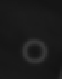
\includegraphics[width=0.4\textwidth]{sift_template.pdf}
    \caption{Modell eines Bohrpunktes (Vergrößert)}
    \label{fig:sift_template}
  \end{center}
\end{figure}


Auf dieses Template wird nun der besprochene SURF Algorithmus angewandt, um die Merkmalsvektoren des Bohrpunktes zu extrahieren.
Das Template wurde dabei bewusst so klein gewählt, dass das Verfahren genau einen Merkmalsvektor liefert, welcher den Bohrpunkt repräsentiert:
\begin{figure}[H]
  \begin{center}
    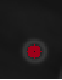
\includegraphics[width=0.4\textwidth]{template_merkmal.pdf}
    \caption{Bohrpunkt mit eingezeichnetem Merkmalsvektor (Vergrößert)}
    \label{fig:template_merkmal}
  \end{center}
\end{figure}

Im nächsten Schritt werden die Merkmalsvektoren im Suchbild extrahiert, wobei wieder der SURF-Algorithmus zum Einsatz kommt, und eine Liste mit Merkmalsvektoren liefert. Zur Illustration werden auch hier die Orte der Merkmalsvektoren in das Suchbild gezeichnet:
\begin{figure}[H]
  \begin{center}
    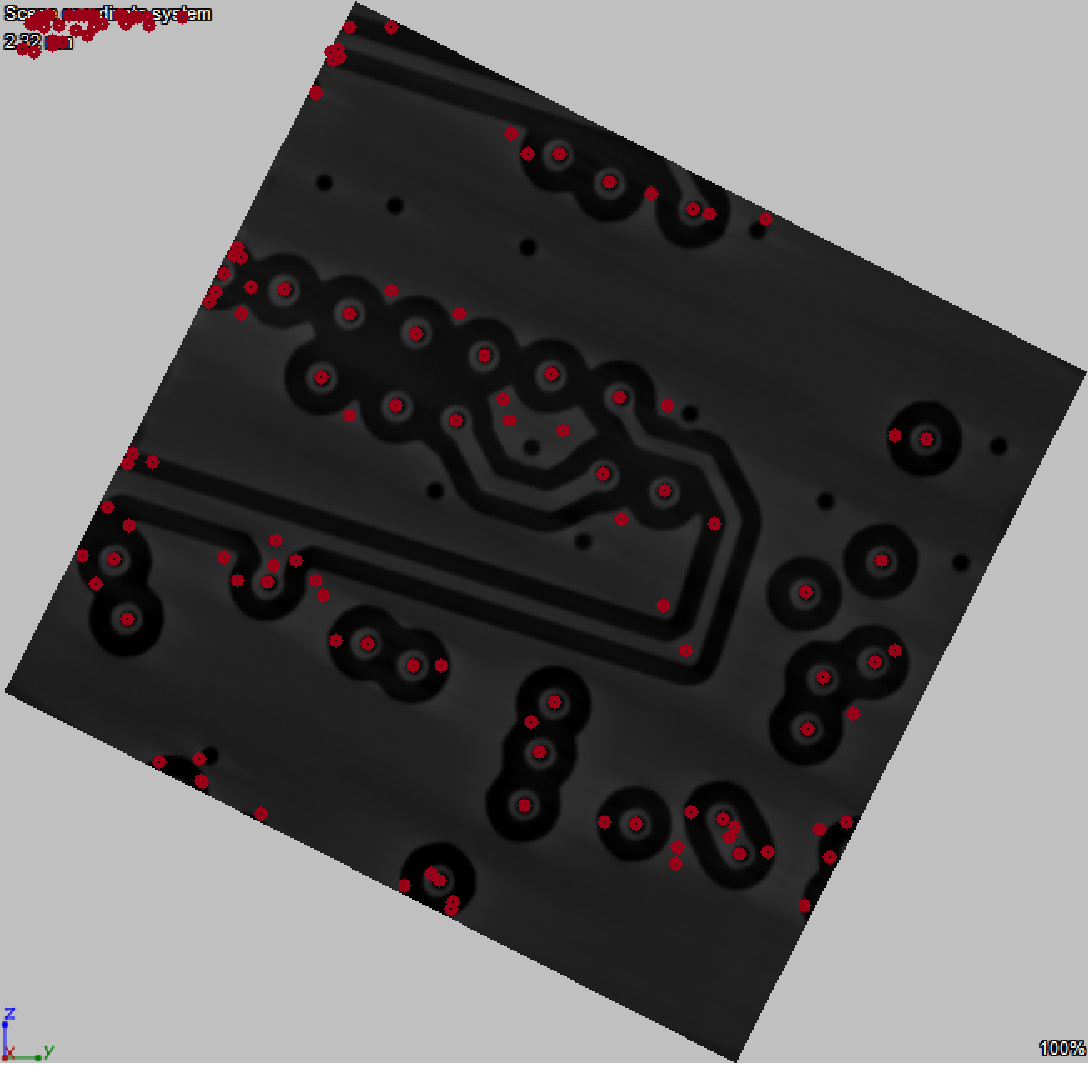
\includegraphics[width=0.8\textwidth]{keypoints.pdf}
    \caption{Suchbild mit eingezeichneten Merkmalsvektoren}
    \label{fig:suchbild_merkmal}
  \end{center}
\end{figure}

Anschließend wird für den Merkmalsvektor des Templates nach Übereinstimmungen in der Liste der Merkmalsvektoren des Suchbildes gesucht, d.h. es wird nach Merkmalsvektoren gesucht, die dem des Templates möglichst ähnlich sind. Ähnlich bedeutet hier, dass die Komponenten zweier Merkmalsvektoren eine hohe Übereinstimmung haben, was genau dann der Fall ist, wenn beide Merkmalsvektoren einen geringen Abstand im Merkmalsraum haben. \\
Daher wird der euklidische Abstand des Merkmalsvektors des Templates mit jedem Merkmalsvektor der Liste berechnet. Ist der Abstand dabei kleiner als $0,45$ im Merkmalsraum, wird eine Übereinstimmung der beiden Merkmalsvektoren angenommen.\\
Dabei werden folgende übereinstimmende Merkmalsvektoren gefunden:
\begin{figure}[H]
  \begin{center}
    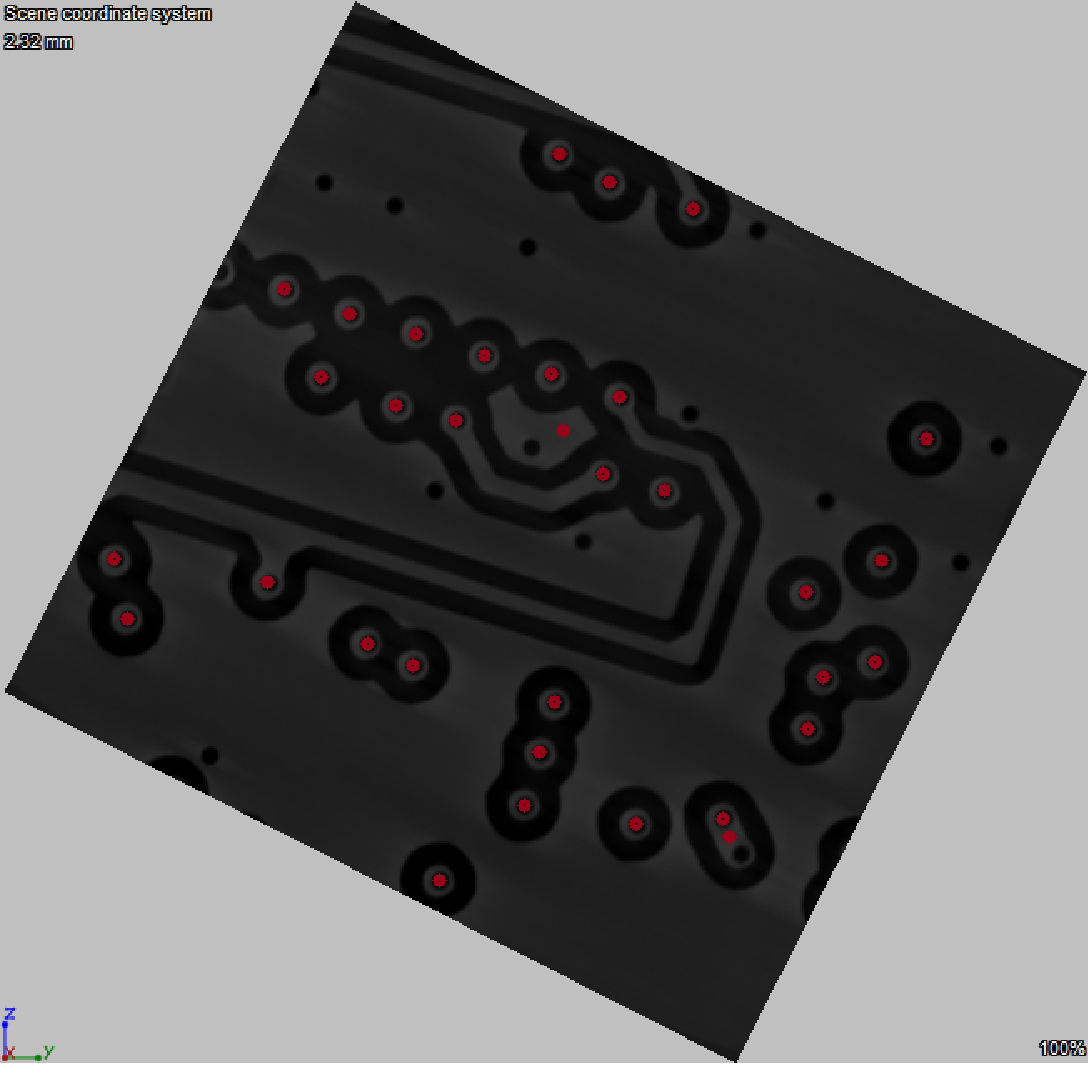
\includegraphics[width=0.8\textwidth]{matches.pdf}
    \caption{Suchbild mit eingezeichneten übereinstimmenden Merkmalsvektoren}
    \label{fig:suchbild_merkmal_matches}
  \end{center}
\end{figure}

Wie deutlich zu sehen ist, werden Borpunkte, die visuell dem Template entsprechen (Bohrpunkt mit äußerer Isolierschicht) fehlerfrei erkannt. Allerdings werden die Bohrpunkte ohne isolierschicht nicht erkannt. Dieser Umstand lässt sich durch eine Modifikation des Suchverfahrens verbessern.

\section{Erweiterung der Merkmalssuche}

Wie im vorigen Abschnitt gezeigt wurde, erkennt das Verfahren des Matchings mit von SIFT-Merkmalen bei einem einzelnen Bild nicht zufriedenstellend, da die Merkmale der Bohrpunkte ohne Isolierschicht nicht eine zu große Distanz zum Merkmalsvektor des Templates im Merkmalsraum haben. \\
Allerdings zeigt sich, dass in Bilder, die sich im Bilderstack nahe am im vorigen Kapitel untersuchten Bild befinden, diese Bohrpunkte erkannt werden. Daher beschränkt man hier die Merkmalssuche nicht auf ein einzelnes Bild, sondern erweitert die Suche auf eine Teilmenge des Bilderstacks. Dabei werden jeweils die $20$ Bilder des Bilderstacks untersucht, die dem Ausgangsbild am nächsten sind. \\
Die in diesen 20 Bildern gefundenen Merkmalsvektoren werden anschließend gemerged, d.h. Merkmalsvektoren die mehrfach vorkommen, werden verworfen, so dass von ihnen jeweils nur ein Merkmalsvektor übrig bleibt. Dieses Merging wird wieder mithilfe des euklidischen Abstands im Merkmalsraum vollzogen: Ist der Abstand zweier Merkmalsvektoren im Merkmalsraum geringer als eine bestimmt Schwelle, werden diese als gleich angesehen und ein Merkmalsvektor wird verworfen. Die Orte der verbleibenden Merkmalsvektoren werden wieder im Bild markiert:
\begin{figure}[H]
  \begin{center}
    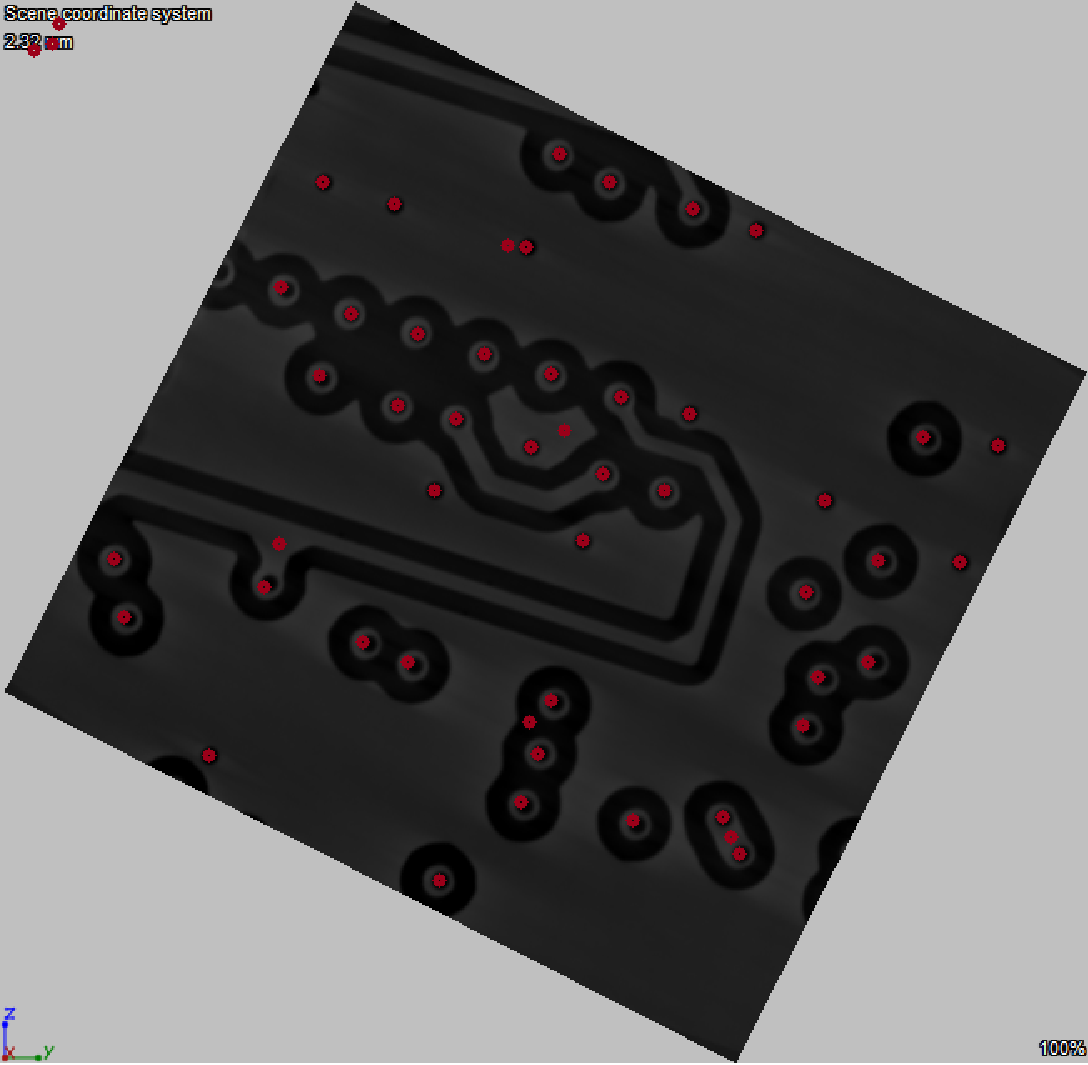
\includegraphics[width=0.8\textwidth]{matches2.pdf}
    \caption{Suchbild mit eingezeichneten gemergeten Merkmalsvektoren}
    \label{fig:suchbild_merge_matches}
  \end{center}
\end{figure}

Bis auf wenige Fehler in Form von Merkmalsvektoren, die keine Bohpunkte beschreiben, werden auf diese Art und Weise alle Bohrpunkte, egal ob mit oder ohne Isolierschicht, erkannt. \\
Dieses Verfahren eignet sich somit vor allem dann, wenn mehrere Unterschiedliche Bilder der gleichen Szene existieren (was in dem zu untersuchenden Bilderstack der Fall ist).
 

\section{Template Matching}
	Template Matching ist ein Verfahren, bei dem ein prototypisches Modell einer Struktur im Bild gesucht wird. Das Template ist dabei selbst ein kleines Bild, welches wie ein Filterkern über das Bild wandert.
\begin{figure}[H]
  \begin{center}
    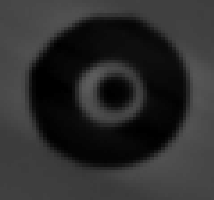
\includegraphics[width=0.6\textwidth]{template.pdf}
    \caption{Template eines Bohrpunktes (Vergrößert)}
    \label{fig:template}
  \end{center}
\end{figure}
Dabei wird in jedem Punkt $(x, y)$ ein Änhlichkeitsmaß des Templates gegenüber dem Bild berechnet.
Ein häufig verwendetes Änglichkeitsmaß ist dabei \textbf{Mean absolute difference (MAD)}.
Dieses Änhlichkeitsmaß bezeichnet die mittlere Differenz der Grauwerte des Bildes $g$ und des Templates $T$:
\begin{equation*}
MAD(x, y) = \frac{1}{M \cdot N} \sum_{ij}^{{}} \left | g(x +i, y + j) - T(i, j) \right |
\end{equation*}
Befindet sich bei der Suche das Template genau über der gesuchten Struktur, ist $MAD(x, y)$ minimal, während bei keiner Übereinstimmung des Templates und des Bildausschnittes $MAD(x, y)$ groß ist. Dadurch sind im resultierenden Bild, in dem das Änhlichkeitsmaß abgebildet wird, lokale Minima die Orte, in denen sich die Struktur des Templates befindet.
\begin{figure}[H]
  \begin{center}
    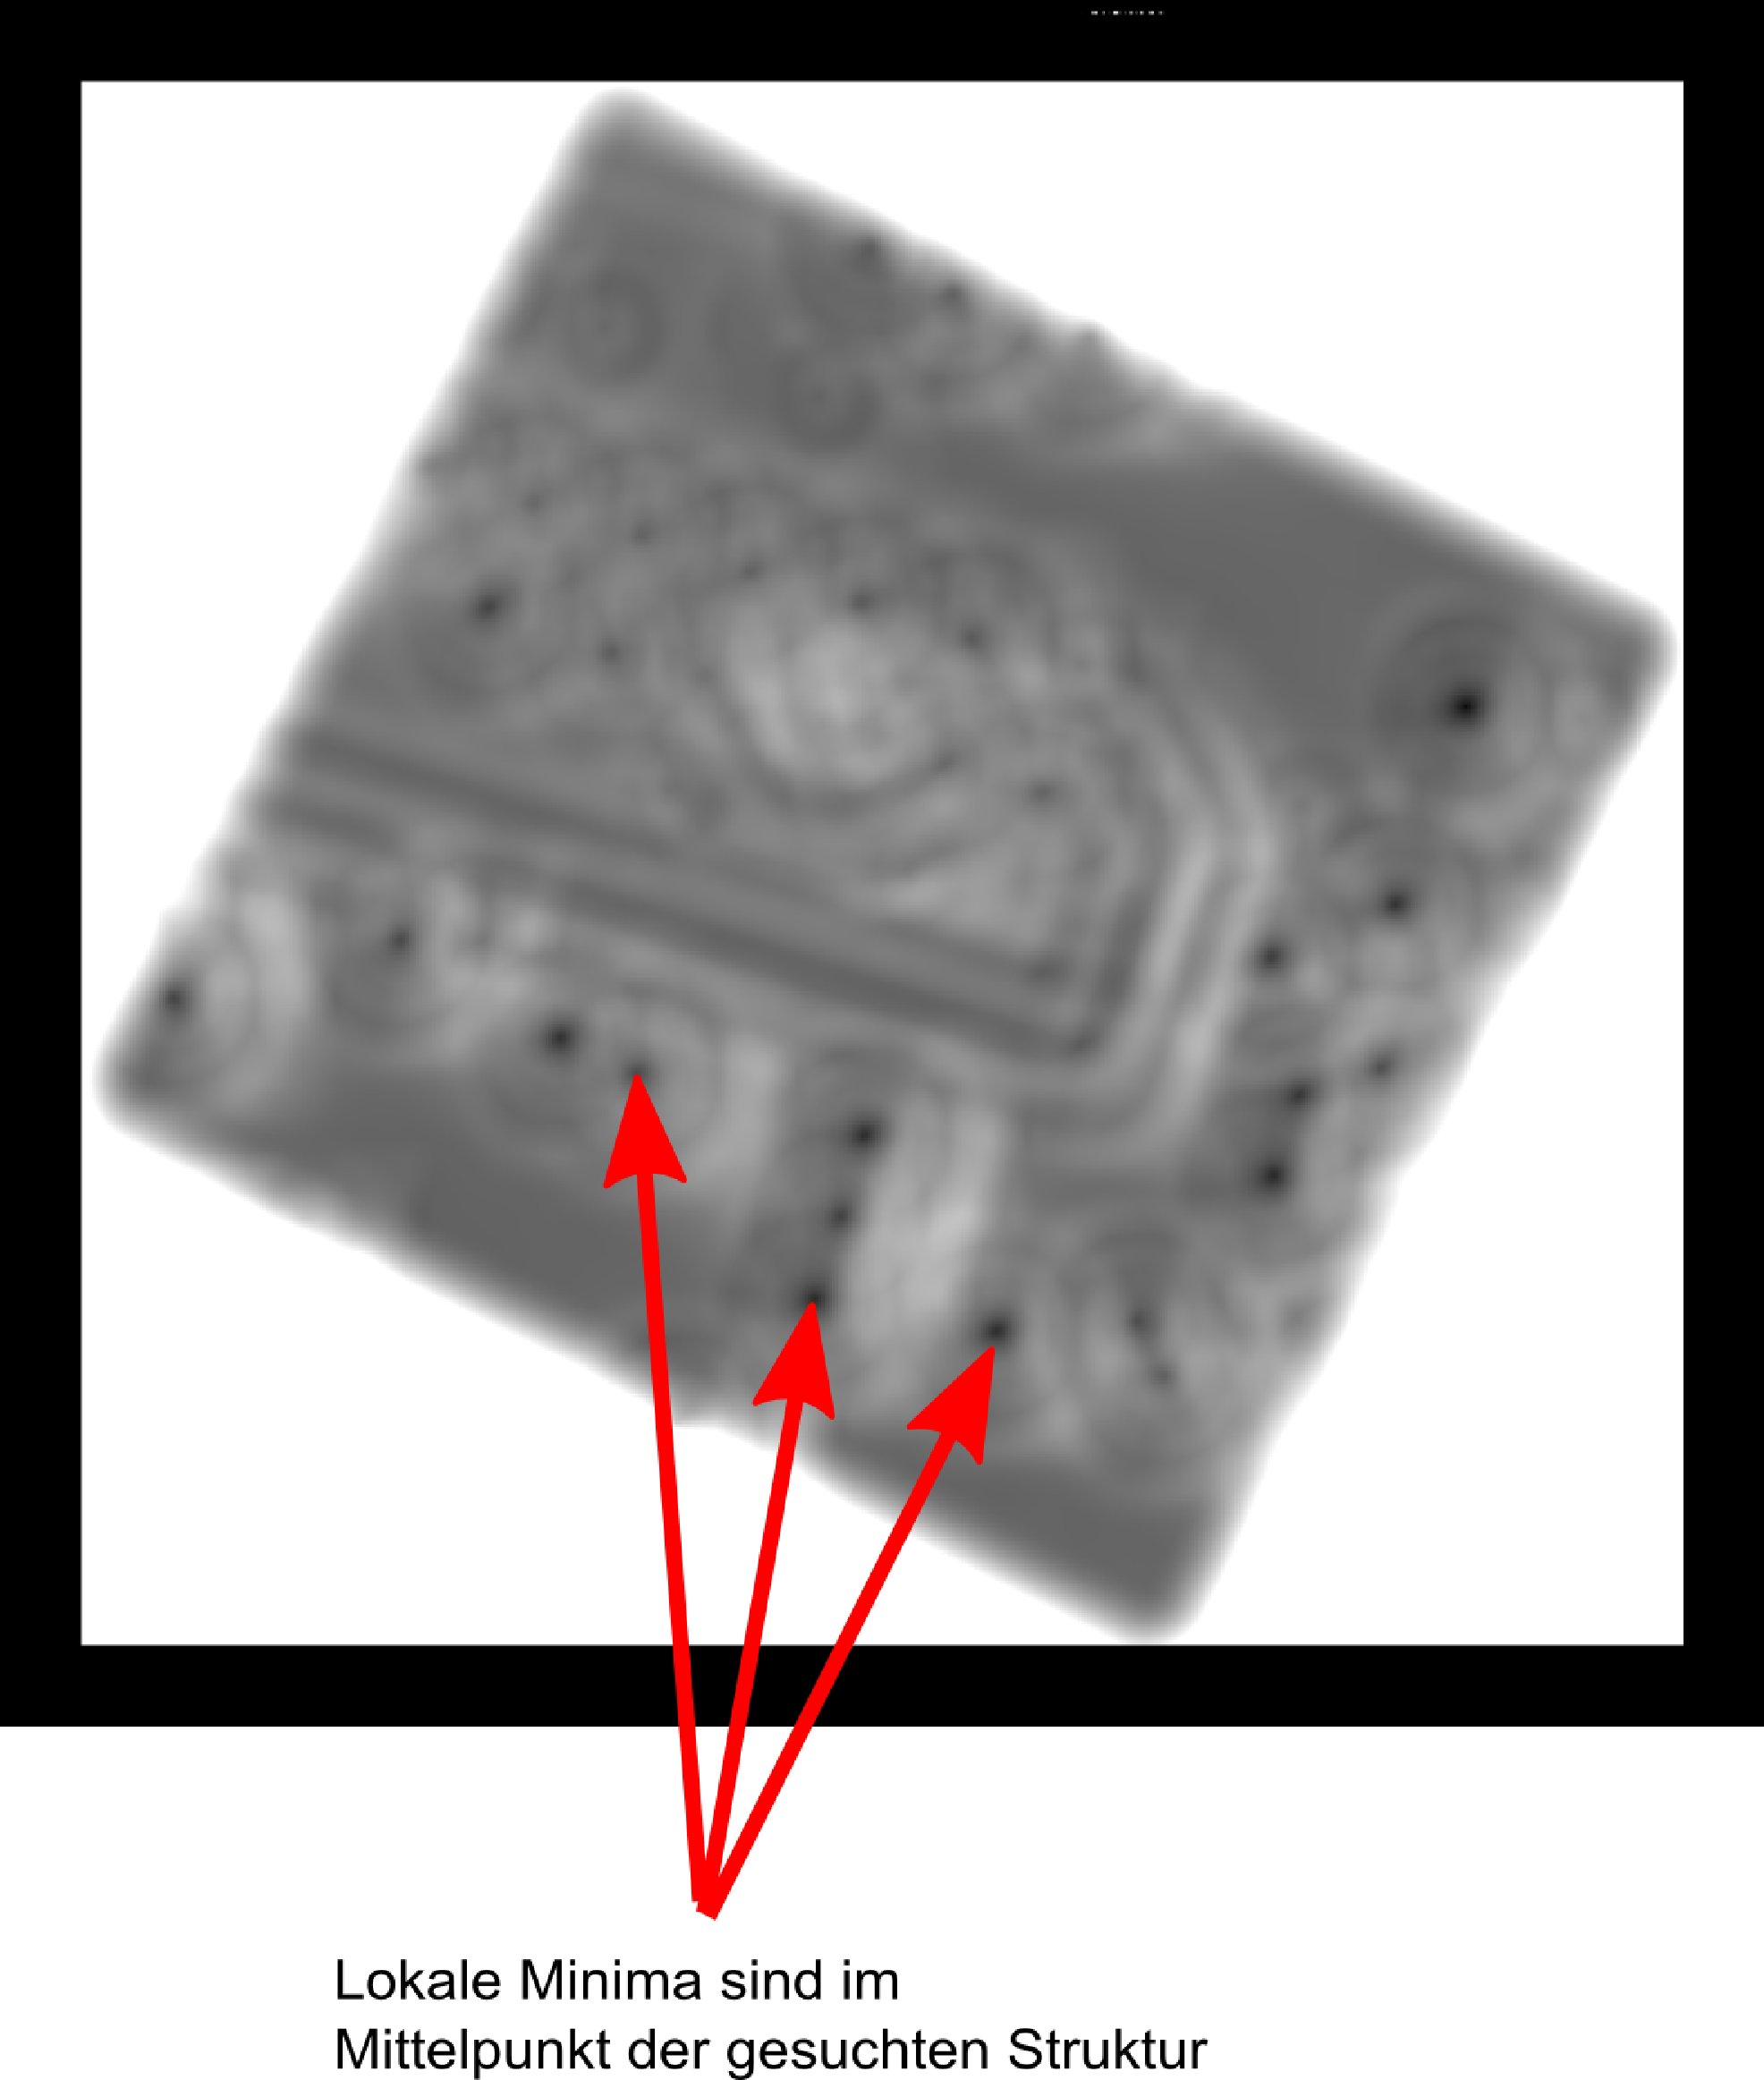
\includegraphics[width=0.7\textwidth]{loc_min.pdf}
    \caption{Lokale Minima}
    \label{fig:localminima}
  \end{center}
\end{figure}

Um die genaue Position der Bohrpunkte zu ermitteln, müssen diese Minima detektiert werden.\\
Der einfachste Ansatz dafür, ist ein Schwellwert zu benutzen, sodass nach der Schwellwertbildung lediglich die lokalen Minima übrig bleiben.
\begin{figure}[H]
  \begin{center}
    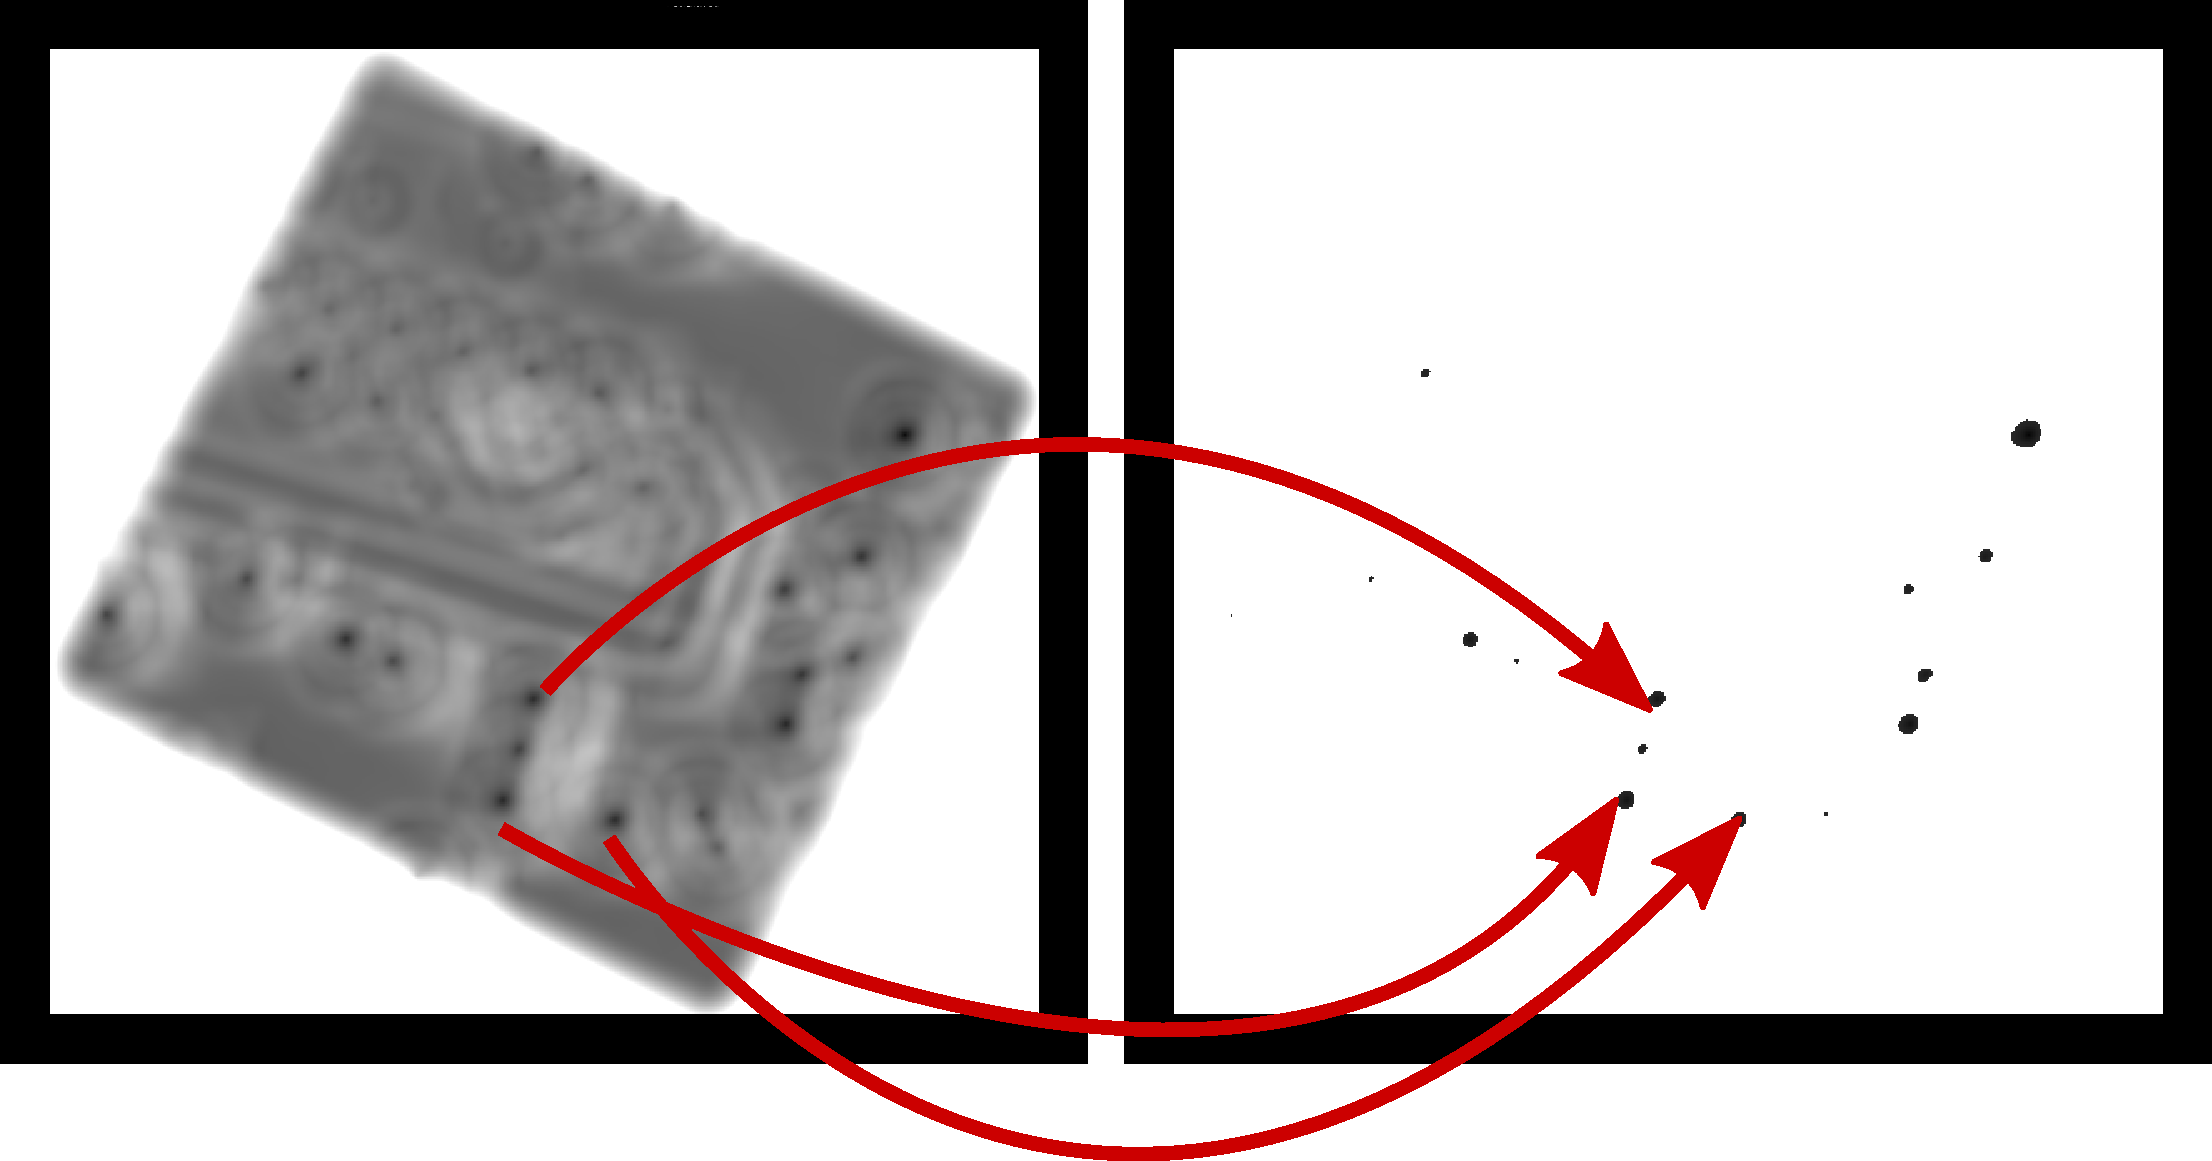
\includegraphics[width=0.9\textwidth]{template_matches.pdf}
    \caption{Lokale Minima nach der Schwellwertbildung}
    \label{fig:localminima_threshold}
  \end{center}
\end{figure}

Ein Problem bei diesem Verfahren ist, den richtigen Schwellwert zu treffen. Ein zu niedriger Schwellwert lässt die lokalen Minima verschwinden. Ein zu hoher Schwellwert führt zu einem "auslaufen" der lokalen Minima in die angrenzenden Regionen.
\begin{figure}[H]
  \begin{center}
    
\includegraphics[width=0.5\textwidth]{template_threshold.pdf}
    \caption{Auslaufen der lokalen Minima bei zu hohem Schwellwert}
    \label{fig:localminima_threshold_bad}
  \end{center}
\end{figure}

Dieser Umstand macht eine automatisierte Suche nach den lokalen Minima schwierig und für die hier betrachteten Daten ungeeignet.


\section{Einsatz der Houghtransformation zur Erkennung von Bohrpunkten}
Da gleichartige Bohrungen wohl auf der kompletten Platine den gleichen Radius (mit einer kleinen Toleranz) besitzen, kann auf 2d-Slices explizit nach Kreisen mit diesem Radius gesucht werden. Dies ergibt für Houghtransformation für Kreise mit Radius = 5 beispielsweise folgendes Bild im Akkumulatorraum:

\begin{figure}[H]
  \begin{center}
    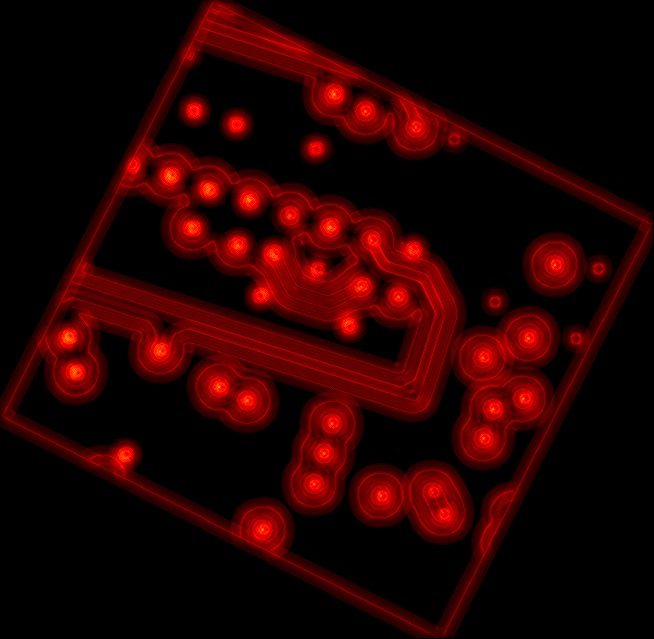
\includegraphics[width=0.7\textwidth]{houghkreiseakku.jpg}
    \caption{Akkumulatorraum für Kreise mit Radius = 5}
    \label{fig:houghkreiseakku}
  \end{center}
\end{figure}

Da die Radien jedoch leicht schwanken, was insbesondere durch die geringe Auflösung bedingt ist, kann beispielsweise noch der Raum für Kreise mit Radius 4 hinzuaddiert werden, um ein klareres Bild zu erhalten. 

\begin{figure}[H]
  \begin{center}
    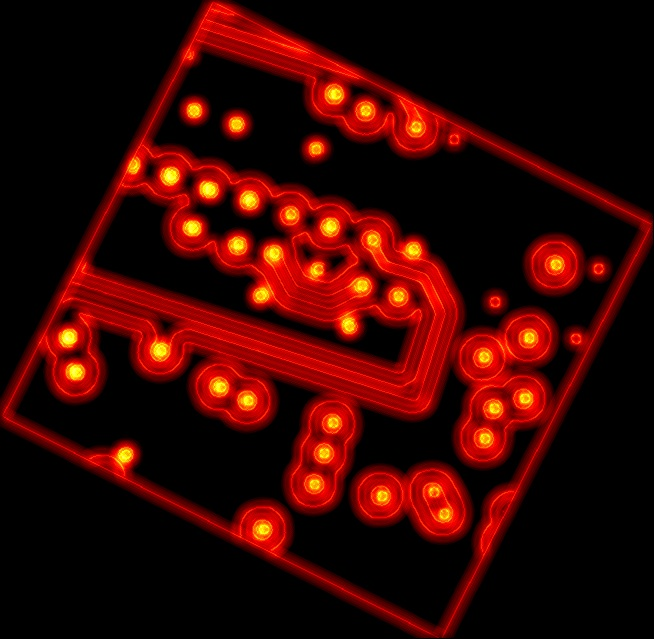
\includegraphics[width=0.7\textwidth]{houghkreiseakku2.jpg}
    \caption{Akkumulatorraum für Kreise mit r=4 und r=5}
    \label{fig:houghkreiseakku2}
  \end{center}
\end{figure}

In diesem Raum müssen nun die lokalen Maxima gefunden werden. Dies ist keine triviale Aufgabe, da ein lokales Maxima in einem anderen Bildbereich eher zum oberen Durchschnitt gehört. Es bietet sich hier der Einfachheit halber dennoch an, alle Pixel oberhalb eines Schwellwertes (z.B $0.6 \cdot globMax$) zu Clustern zusammenfassen und aus diesen jeweils den Mittelpunkt als Bohrung zu speichern. 

\begin{figure}[H]
  \begin{center}
    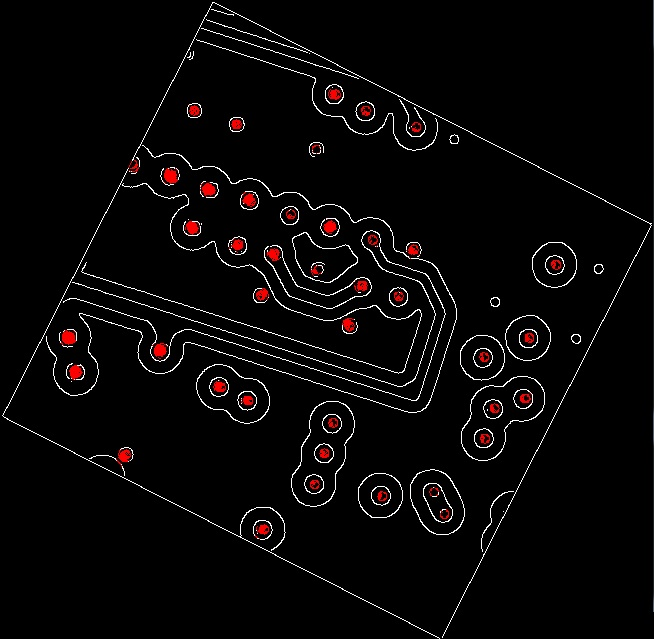
\includegraphics[width=\textwidth]{canny_HoughRes.jpg}
    \caption{Pixel mit höherem Wert als $0.6 \cdot globMax$}
    \label{fig:houghkreiseakku2}
  \end{center}
\end{figure}

Wendet man ein solches Schwellwertverfahren an, so müsste der Schwellwert heuristisch optimiert werden, um möglichst viele Punkte zu “erwischen”, da Bohrungen ohne umliegende Kanten (bspw. Isoliermaterial) generell schächer in den Akkumulatorraum abgebildet werden. \newline
Um dieses Bild zu verbessern, hat man natürlich die Möglichkeit den Akkumulatorraum mit verschiedenen Filtern zu falten, um damit bspw. alle kreisförmigen Maxima zu verstärken. \newline
Ansonsten könnte man beispielsweise verschiedene “Hill-Climbing”-Algorithmen einsetzen, wobei hier zu beachten ist, dass ein lokales Maximum nur dann als Hinweis für eine Bohrung interpretiert werden darf, wenn die Menge zusammenhängender, umgebender Pixel mit ähnlich hohem Wert lokal relativ beschränkt ist. Dadurch werden nur “punktförmige” Maxima gefunden.

\section{Alternativer Algorithmus zur Erkennung von Bohrpunkten auf Grundlage einer Färbung}
Die Houghtransformation für Kreise ist relativ rechenintensiv und schließlich muss der Akkumulatorraum noch ausgewertet werden. Auch das Templatematching arbeitet mit Filterkernen, die so groß sind wie die gesuchten Kreise. Dies motivierte dazu einen schnelleren Algorithmus zu entwickeln, zur Not auch auf Kosten der Universalität.
Eine sehr einfache und effiziente Möglichkeit Kreise in einem Canny-Edge Bild zu finden ist die folgende:
\newline
%\begin{Algorithmus}
%\caption{Algorithmus in Pseudocode}
%\label{alg:sample}
\begin{algorithmic}
\Procedure{FindHoles}{Bild $img$, Radius $r$, Toleranz $t$}
\ForAll{Pixel $p \in img$}
  \If{$p$ ist weiß}
    \State Folge der zugehörigen weißen Linie $l$ ungefähr $n$ Schritte lang
    \State , wobei $n <= int(2\cdot\pi\cdot(r+t))$
      \ForAll{Mittelpunkte $mp$}\Comment Geschätzt aus der Position von $p$.
        \If{$\exists lp \in l: dist(mp, lp) < r - t \lor dist(mp, lp) > r + t $}
          \State Abbrechen             
        \EndIf 
        \If{Die Linie umschließt den Mittelpunkt (z.B. Quadrantencheck)}
          \State l sei ein Kreis; continue in äußerer Schleife            
        \EndIf
      \EndFor
  \EndIf
\EndFor
\EndProcedure \newline
\end{algorithmic}
%\end{Algorithmus}

\begin{figure}[H]
  \begin{center}
    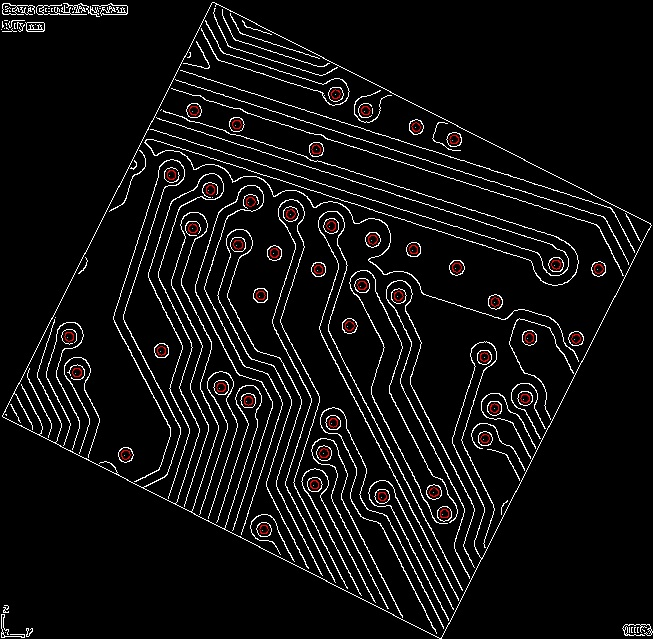
\includegraphics[width=\textwidth]{canny2_PA1.jpg}
    \caption{Ein Resultat des Algorithmus (gefundene Bohrungen sind rot markiert)}
    \label{fig:b_alg_1}
  \end{center}
\end{figure}


\subsection{Bewertung:}
Der Algorithmus ist extrem schnell und erkannte in sämtlichen Testbildern ohne Probleme alle gesuchten Kreise. Falls die Kantendetektion einen Fehler gemacht hat und der Kreis eine kleinere Lücke beinhaltet, so wird der Kreis im allgemeinen dennoch erkannt (Falls die Lücke nicht zu groß ist). \newline
Problematisch könnte selbstverständlich die Verallgemeinerung auf die gleichzeitige Suche von Kreisen beliebiger Radien werden. Diesbezüglich wurden noch keine Anstrengungen unternommen, da hierfür noch keine Notwendigkeit bestand.

\section{Einsatz der Houghtransformation zur Erkennung von Leiterbahnen}
Die Houghtransformation ist nicht direkt geeignet für das Erkennen von Leiterbahnen, da ausschließlich Geradenstücke erkannt werden. Aus Diesen lässt sich jedoch nicht schließen, ob es sich um eine Leiterbahn handelt oder nicht (es könnte z.B. auch Teil von Isoliermaterial sein). \newline
Die Kurven der Bahnen werden nicht erkannt, somit müsste man die Geradenstücke manuell verlinken und anschließend noch jeweils 2 Kanten (Bahnränder) zu einer Leiterbahn zusammenfassen. Zudem müssten andere, im Bild vorkommende Geraden ausgeschlossen werden. \newline
Dieses Anpassungsverfahren scheint also um relativ kompliziert zu sein, da es einfachere Wege gibt die Bahnen zu finden.  

\section{Alternativer Algorithmus zu Erkennung von Leiterbahnen auf Grundlage einer Färbung}
Bohrungen sind relativ einfach zu finden, weil es sich um einigermaßen simple geometrische Objekte handelt. Da alle Leiterbahnen schließlich in einer Bohrung enden, motiviert die Idee einen Algorithmus zu schreiben, der bei bereits erkannten Bohrungen prüft, ob eine Leiterbahn in sie mündet.\newline
Ein Beispiel für einen solchen Algorithmus wäre folgendes Verfahren: \newline
\begin{enumerate}
\item Man zeichne einen Kreis $k1$, dessen Radius etwas größer ist als der Abstand vom Mittelpunkt der Bohrung bis zum äußeren Ende der umgebenden Isolierschicht. \newline
Da die gefundenen Bohrpunkte nicht immer perfekt in der Mitte liegen, untersucht man auch die Umgebungen jedes Bohrpunktes.
\item Falls in diesem Kreis ausgenommen von “weiß” und “schwarz” nur zwei Farben vorkommen, so weiß man, dass es sich entweder um eine Bohrung mit Leiterbahn handelt, oder aus Versehen eine “fremde” Region geschnitten wurde. 
\item Betrachtet man das Vorkommen der selteneren Farbe in einem Kreis $k2$, dessen Radius etwas kleiner ist, als der Radius von $k1$, so kann man anhand eines einfachen Vergleichs des Mengenverhältnisses in $k1$ und $k2$ schätzen, dass es sich um ein Leiterbahn handeln kann. \newline
Dies liegt daran, dass die Farbe der Leiterbahn in beiden Kreisen in ungefähr gleich vielen Pixeln auftauchen muss (im inneren Kreis evtl. etwas häufiger).
\end{enumerate}

\begin{figure}[H]
  \begin{center}
    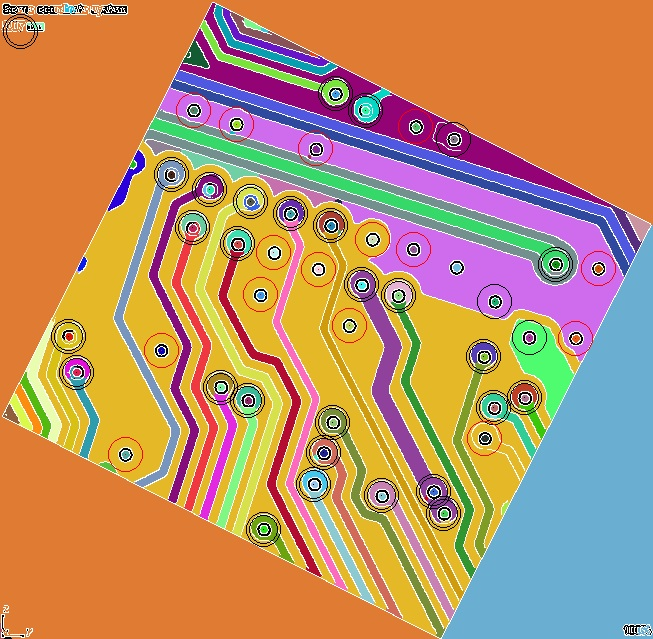
\includegraphics[width=\textwidth]{canny2_FACA1_test.jpg}
    \caption{Eingezeichnete Kreise (bei roten Kreisen ist bereits das Kriterium aus Schritt zwei verletzt.)}
    \label{fig:l_alg_1_test}
  \end{center}
\end{figure}

\begin{figure}[H]
  \begin{center}
    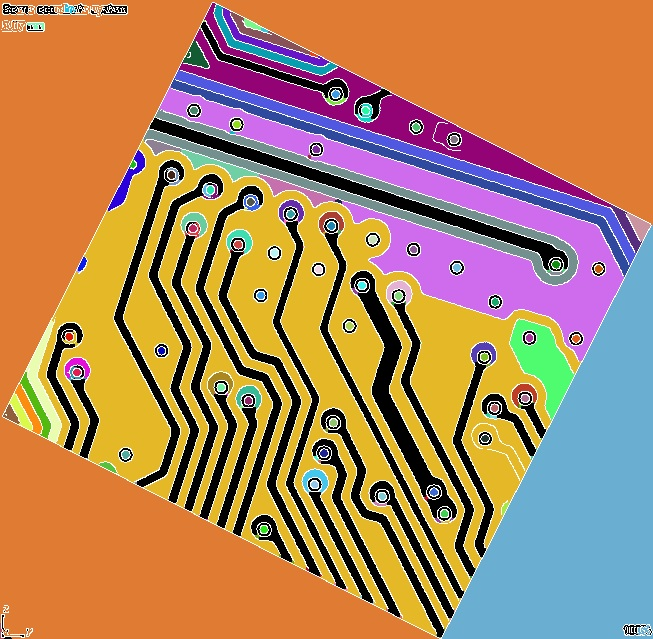
\includegraphics[width=\textwidth]{canny2_FACA1.jpg}
    \caption{Ein Resultat des Algorithmus (gefundene Leiterbahnen sind schwarz markiert)}
    \label{fig:l_alg_1}
  \end{center}
\end{figure}

\subsection{Bewertung:}
Der Algorithmus ist relativ schnell, da er nur die bereits gegebenen Bohrungen untersucht und nicht daher nicht das komplette Bild durchforstet. \newline
Gegenüber Fehlern im “Canny”-Bild ist der Algorihtmus nur insofern robust wie es der verwendete Färbealgorithmus ist. \newline
Problematisch ist natürlich auch hier, dass der Algorithmus speziell auf das Problem zugeschnitten wurde und daher an Universalität einbüßt.

\section{Weiterer alternativer Algorithmus zu Erkennung von Leiterbahnen}
Da der vorherige Algorithmus von Robustheit des Färbealgorithmus abhängt und daher im Allgemeinen anfällig ist für Fehler des Canny-Edge-Detektors, wäre ein Algorithmus interessant, welcher ohne Färbung auskommt. \newline
Da die Bohrungen bisher zuverlässig erkannt wurden und es das Verfahren extrem beschleunigt, soll auch hier wieder von den gefundenen Bohrungen ausgegangen werden. \newline
Der hier vorgeschlagene, auf das Problem abgestimmte Algorithmus sucht im Wesentlichen die Kante(n) einer eventuellen Leiterbahn und untersucht ihr Verhalten bezüglich der Umrundung des Bohrpunktes: \newline

\begin{enumerate}
\item Man zeichne wieder einen Kreis, dessen Radius etwas größer ist als der Abstand vom Mittelpunkt der Bohrung bis zum äußeren Ende der umgebenden Isolierschicht. \newline
Da die gefundenen Bohrpunkte nicht immer perfekt in der Mitte liegen, untersucht man auch die Umgebungen jedes Bohrpunktes.
\item Falls es auf dem Kreis genau zwei weiße Cluster gibt und deren euklidischer Abstand im Toleranzbereich der Breite einer Leiterbahn liegt, so kann man sagen, dass es sich entweder um die beiden Seiten der Leiterbahn handelt oder keine Leiterbahn von der Bohrung ausgeht und zufällig zwei fremde Punkte mit dem richtigen Abstand gefunden wurden.
\item Um letzteren Fall mit hoher Wahrscheinlichkeit auszuschließen könnte man beispielsweise jeweils der zugehörigen weißen Linie eines Clusters folgen und schließlich untersuchen, ob die Vereinigung der beiden Linien den Bohrpunkt umrundet (bspw. Quadrantencheck: Liegen in jedem Quadranten um den Bohrpunkt min. x Pixel?).
\end{enumerate}

\begin{figure}[H]
  \begin{center}
    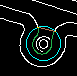
\includegraphics[width=0.7\textwidth]{CA1.png}
    \caption{Beispiel zu Verdeutlichung: Der in Schritt 1 gezeichnete Kreis ist blau; Die gefundenen Cluster sind gelb; Der gemessene Abstand ist braun; Die Vereinigung der beiden Linien grün.}
    \label{fig:l_alg_1}
  \end{center}
\end{figure}

Um nun die tatsächliche Leiterbahn zu extrahieren könnte man beispielsweise den Floodfill Algorithmus der braunen Linie im Bild starten und somit alle Pixel der Leiterbahn zu finden. Das würde jedoch dem Vorhaben widersprechen, ohne Färbung und der damit verbunden, bereits angesprochenen Schwäche auszukommen. \newline
Daher bietet es sich beispielsweise folgendes Verfahren zur Extraktion der Leiterbahnen an (Die Leiterbahnen machen keine scharfen Kurven): \newline

\begin{enumerate}
\item Man schießt einen Strahl, ausgehend vom Bohrpunkt in Richtung Leiterbahn, dh. durch die Mitte der gezeichneten, braunen Linie.
\item Der Strahl wird am Punkt p gestoppt, und zwar $n$ Pixel vor einer weißen Linie.
\item Anschließend vergleicht man $n$ mit $n_{links}$ und $n_{rechts}$, welche entstehen, wenn man, anstatt von p geradeaus zu gehen um um $45^\circ$ nach links bzw. nach rechts geht. 
\item Den längsten der drei Wege wählt man als neuen Startweg, halbiert den Winkel und macht weiter bei Schritt 3. Durch diesen Trick wird bei den Leiterbahnen für jeden aktuellen Punkt p der längste Weg in die richtige Richtung gefunden (siehe nachfolgende Grafik).
\item Wenn man den längsten Strahl ausgehend vom Punkt p gefunden hat, dann wird p neu gesetzt, indem man mit diesem Strahl wieder bei Schritt 2 weitermacht. Falls kein neuer Strahl gefunden wurde ist man fertig.
\end{enumerate}

\begin{figure}[H]
  \begin{center}
    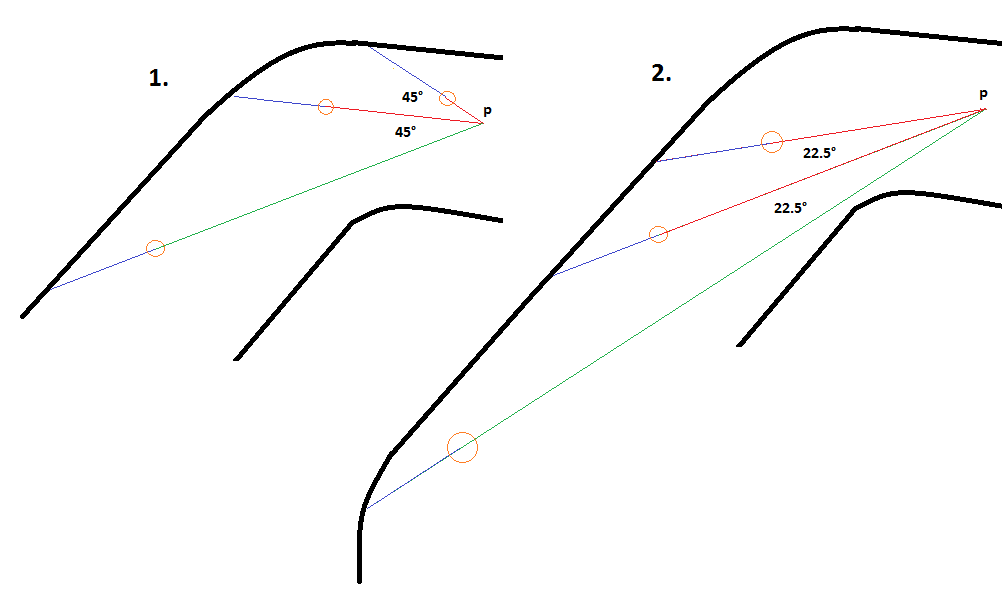
\includegraphics[width=0.7\textwidth]{LinienpunkteMuster.png}
    \caption{Zwei Iterationsschritte zu Verdeutlichung: Der grüne Weg ist jeweils der längste und wird daher als Ausgangsrichtung für die nächste Winkelhalbierung gesetzt.}
    \label{fig:linepoints}
  \end{center}
\end{figure}

Dieses Vorgehen führt dazu, kleinere Lücken im Kantenbild mit einigermaßen hoher Wahrscheinlichkeit übersprungen werden, insbesondere dann, wenn sie auf einem langen, geradlinigen Abschnitt auftauchen. Dieser Vorteil ist im folgenden Bild zu sehen, in welchem auch die Leiterbahn gefunden wurde, welche beim vorherigen Verfahren aufgrund der fehlerhaften Färbung nicht erkannt wurde.

\begin{figure}[H]
  \begin{center}
    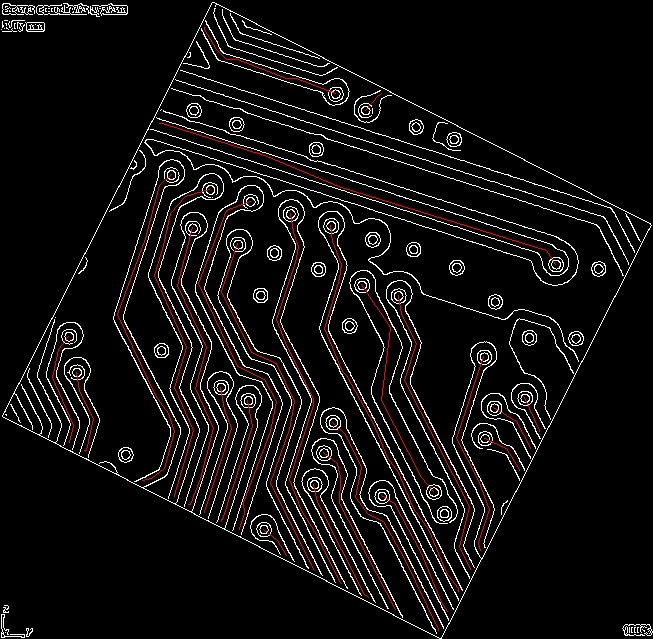
\includegraphics[width=\textwidth]{canny2_CA1_Circuits.jpg}
    \caption{Ein Resultat des Algorithmus (gefundene Leiterbahnen sind rot markiert). Es wurden zusätzlich Leiterbahnen, welche zwischen zwei Bohrungen verlaufen kombiniert.}
    \label{fig:linepoints2}
  \end{center}
\end{figure}

\begin{figure}[H]
  \begin{center}
    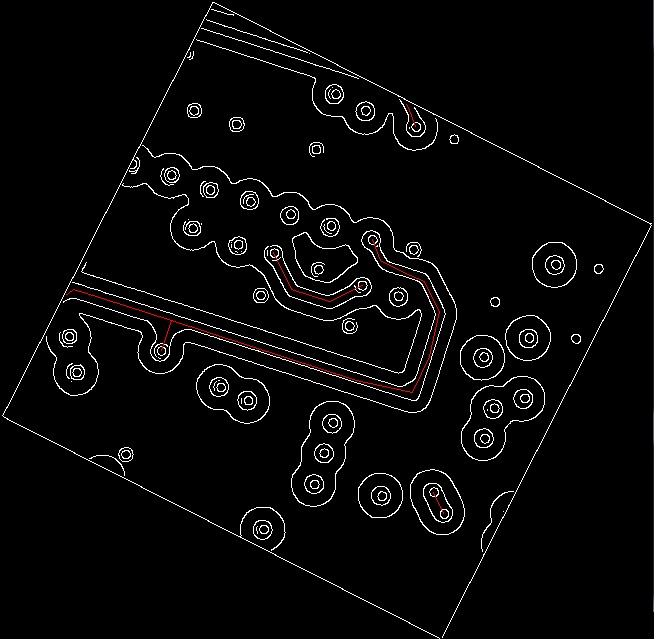
\includegraphics[width=\textwidth]{canny_CA1_Circuits.jpg}
    \caption{Ein anderes Resultat des Algorithmus (gefundene Leiterbahnen sind rot markiert). Außerdem wurden Leiterbahnen, welche zwischen n Bohrungen verlaufen zu einem Graph kombiniert.}
    \label{fig:linepoints22}
  \end{center}
\end{figure}

\subsection{Bewertung:}
Durch die beidseitige Verfolgung der von den Clustern ausgehenden Linien und dem anschließenden Check deren Vereinigung bezüglich dem Quadrantenkriterium hat sich das Verfahren für die Erkennung von Leiterbahnen auch bei Lücken im Canny-Edge-Bild bewährt. \newline
Das Verfahren zur nachfolgenden Extraktion der Leiterbahnen hat in den getesteten Szenarien gut funktioniert und ist einigermaßen einfach zu implementieren. \newline
Wenn ein Strahl jedoch zufällig durch eine Lücke im Kantenbild springt, dann hat das unabsehbare Konsequenzen und die Leiterbahn muss aus der Liste gestrichen werden. Ersteres ist wiederum einem Algorithmus nicht auf trivialem Wege ersichtlich und diesbezüglich müssen weitere Anstrengungen unternommen werden. \newline
Auch dieser Algorithmus ist extrem schnell und dürfte keinerlei Performanz-Probleme bereiten. 
%Folgende Zeile aktivieren und als SVN property "svn:keywords" auf "Id" setzen, um SVN Versionsinformationen im Dokument zu erhalten
%\svnInfo $Id: einleitung.tex 60 2012-01-26 15:56:06Z koppor $ 

\chapter{3D - Verfahren}
\label{chap:3d}
\subsection{RANSAC}
RANSAC (\textbf{RA}ndom \textbf{SA}mple \textbf{C}onsensus) ist ein iteratives Verfahren zur Schätzung eines mathematischen Models anhand von Beobachtungsdaten mit Ausreißern. Der Algorithmus ist nicht-deterministisch, da ihm probabilistische Ansätze zu Grund liegen. Aufgrund seiner Robustheit wird er häufig im Bereich des maschinellen Sehens eingesetzt. 

\begin{figure}[H]
  \begin{center}
    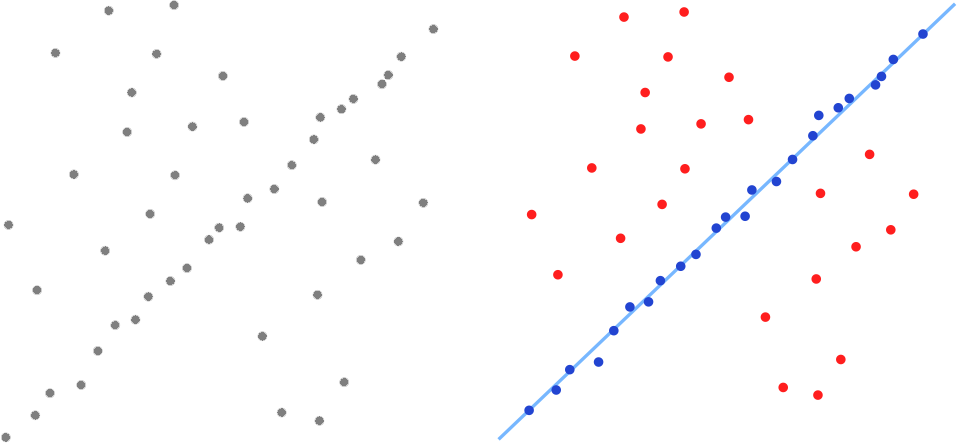
\includegraphics[width=0.9\textwidth]{RANSACline.png}
    \caption{In einen Datensatz mit vielen Ausreißern wird eine Linie eingepasst.}
    \label{fig:l_alg_1}
  \end{center}
\end{figure}

\subsection{Der Algorithmus}
 Für das zu erkennende Objekt wird ein parameterabhäniges Modell erstellt. Danach werden die Daten iterativ auf mögliche Vorkommnisse eines auf das Modell passenden Objekts getestet, dafür werden iterativ zufällige Punkte aus den Daten selektiert und als hypothetische Einlieger des Objekts betrachtet und das Modell an diese Punkte angepasst. Für eine Linie wären dies zwei Punkte um sie ausreichend zu beschreiben. Nun wird das Modell getestet:

\begin{enumerate}
\item Alle anderen Punkte werden gegen das Modell getestet und falls sie dazu passen ebenfalls als mögliche Einlieger gespeichert.
\item Das Modell wird akzeptiert wenn genug Einlieger gefunden werden.
\item Das Modell auf Basis aller gefundenen Einlieger neu berechnet und evaluiert.
\end{enumerate}

Nach ausreichend vielen Iterationen wird das beste Modell benutzt um alle Punkte des Objekts zu identifizieren. Anschließend wird das gefundene Objekt aus den Daten gelöscht und gegebenenfalls nach weiteren Vorkommnissen gesucht.

\begin{figure}[H]
  \begin{center}
    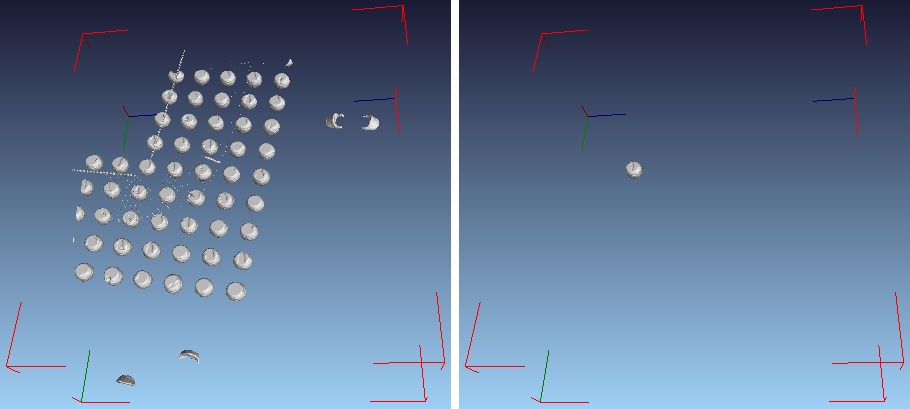
\includegraphics[width=0.9\textwidth]{RANSACball.png}
    \caption{In einem per Threshhold-Verfahren vorverarbeiteten Datensatz wird anhand eines einfachen Modells eine Kugel identifiziert.}
    \label{fig:l_alg_1}
  \end{center}
\end{figure}

\subsection{Bewertung}
Der Algorithmus eignet sich sehr gut um in großen Datenmengen schnell Instanzen von Modellen zu finden. Für den diskutierten Anwendungsfall ist er leider vergleichsweise langsam. Der Grund dafür ist, dass die zu suchenden Objekte schon durch einen Dichte-Threshhold sehr gut vor-isoliert werden können. Man kann sich deshalb direkt darauf konzentrieren einzelne Punktmengen auf bestimmte Eigenschaften hin zu untersuchen. Der große Vorteil von RANSAC schnell mögliche Kandidaten zu entdecken wird deshalb negiert.
%\input{...weitere Kapitel...}
%%Folgende Zeile aktivieren und als SVN property "svn:keywords" auf "Id" setzen, um SVN Versionsinformationen im Dokument zu erhalten
%\svnInfo $Id: kapitel2.tex 62 2012-04-20 15:14:01Z koppor $ 

%Die Angabe des schlauen Spruchs auf diesem Wege funtioniert nur,
%wenn keine Änderung des Kapitels mittels den in preambel/chapterheads.tex
%vorgeschlagenen Möglichkeiten durchgeführt wurde.
\setchapterpreamble[u]{%
\dictum[Albert Einstein]{Probleme kann man niemals mit derselben Denkweise lösen, durch die sie entstanden sind.}
}
\chapter{Tutorialchapter}
%\vspace{-3cm}
%\vspace{2cm}

\label{chap:tut}
Hier wird der Hauptteil stehen. Falls mehrere Kapitel gewünscht, entweder mehrmals \texttt{\textbackslash{}chapter} benutzen oder pro Kapitel eine eigene Datei anlegen und \texttt{ausarbeitung.tex} anpassen.

\section{File-Encoding}
Die Vorlage wurde 2010 auf UTF-8 umgestellt. TeXnicCenter 1 RC 1 unterstützt \textbf{kein} UTF-8. Die Alpha-Version soll UTF-8 können, aber es gibt anscheinend Probleme. Deshalb bitte einen anderen Editor, wie \zB TeXstudio.

\section{Mathematische Formeln}
\label{sec:mf}
Mathematische Formeln kann man $so$ setzen. \texttt{symbols-a4.pdf} (zu finden auf \url{http://www.ctan.org/tex-archive/info/symbols/comprehensive/symbols-a4.pdf}) enthält eine Liste der unter LaTeX direkt verfügbaren Symbole. z.\,B.\ $\mathbb{N}$ für die Menge der natürlichen Zahlen. Für eine vollständige Dokumentation für mathematischen Formelsatz sollte die Dokumentation zu \texttt{amsmath}, \url{ftp://ftp.ams.org/pub/tex/doc/amsmath/} gelesen werden.

Folgende Gleichung erhält keine Nummer, da \texttt{\textbackslash equation*} verwendet wurde.
\begin{equation*}
x = y
\end{equation*}

Die Gleichung~\ref{eq:test} erhält eine Nummer:
\begin{equation}
\label{eq:test}
x = y
\end{equation}

Eine ausführliche Anleitung zum Mathematikmodus von LaTeX findet sich in \url{http://www.ctan.org/tex-archive/help/Catalogue/entries/voss-mathmode.html}.

\section{Quellcode}
Listing~\ref{lst:ListingANDlstlisting} zeigt, wie man Programmlistings einbindet.  Mittels \texttt{\textbackslash lstinputlisting} kann man den Inhalt direkt aus Dateien lesen.

%Listing-Umgebung wurde durch \newfloat{Listing} definiert
\begin{Listing}
\begin{lstlisting}
<listing name="second sample">
  <content>not interesting</content>
</listing>
\end{lstlisting}
\caption{lstlisting in einer Listings-Umgebung, damit das Listing durch Balken abgetrennt ist}
\label{lst:ListingANDlstlisting}
\end{Listing}

Quellcode im \lstinline|<listing />| ist auch möglich.

\section{Abbildungen}
Die Abbildungen~\ref{fig:chor1} und~\ref{fig:chor2} sind für das Verständnis dieses Dokuments
wichtig. Im Anhang zeigt Abbildung~\vref{fig:AnhangsChor} erneut die komplette Choreographie.

%Die Parameter in eckigen Klammern sind optionale Parameter - z.B. [htb!]
%htb! bedeutet: "Liebes LaTeX, bitte platziere diese Abbildung zuerst hier ("_h_ere"). Falls das nicht funktioniert, dann bitte oben auf der Seite ("_t_op"). Und falls das nicht geht, bitte unten auf der Seite ("_b_ottom"). Und bitte, bitte bevorzuge hier und oben, auch wenn's net so optimal aussieht ("!")
%Diese sollten nach Möglichkeit NICHT verwendet werden. LaTeX's Algorithmus für das Platzieren der Gleitumgebung ist schon sehr gut!
\begin{figure}
  \begin{center}
    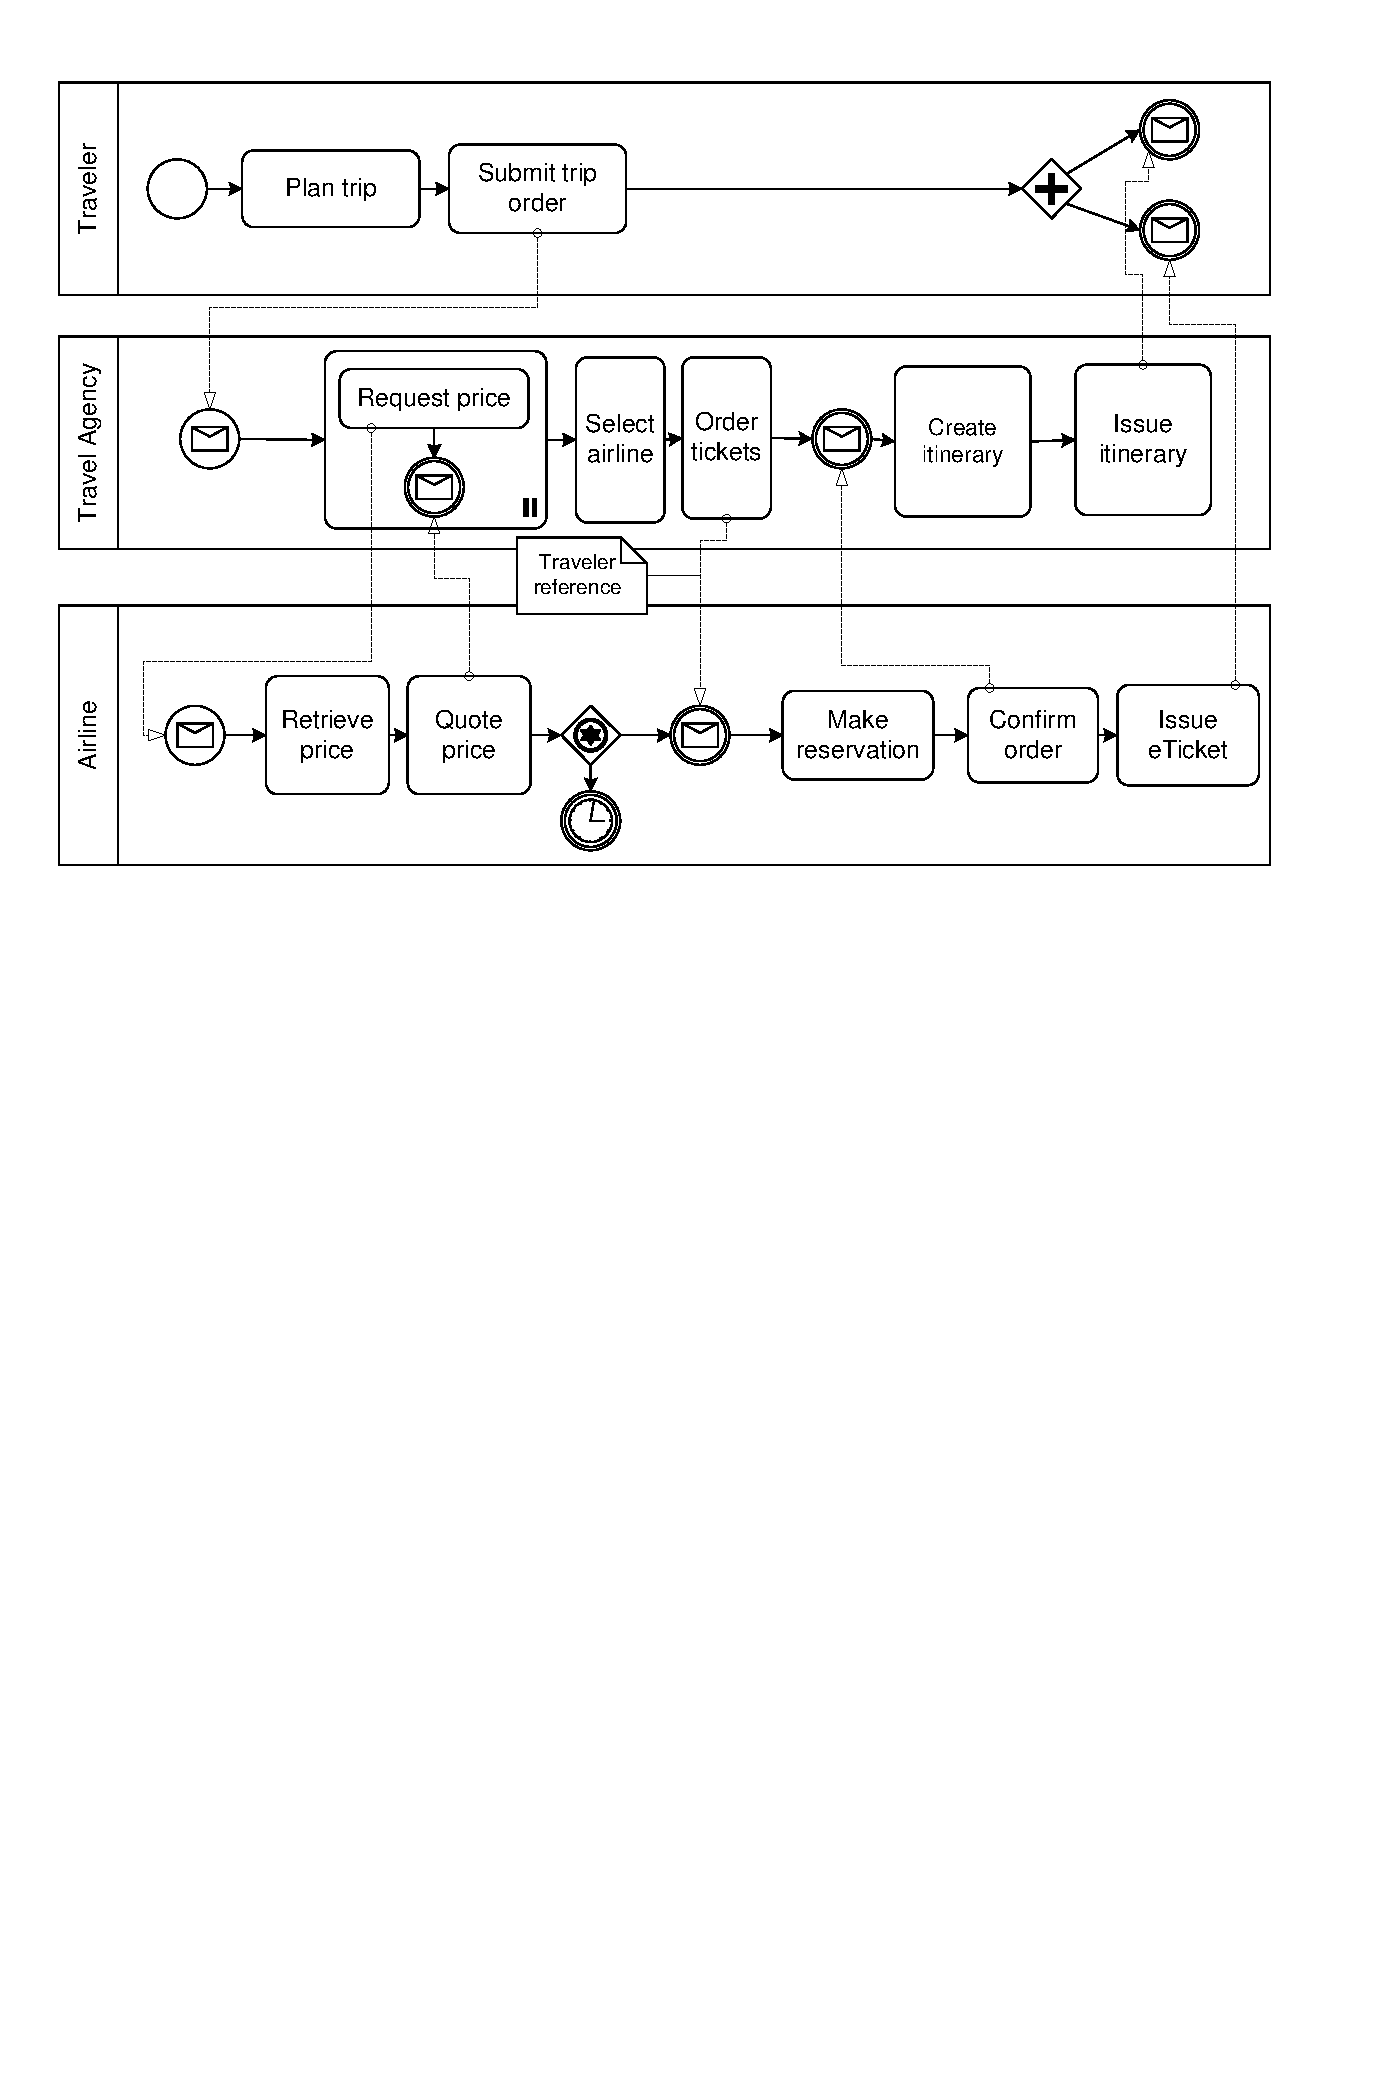
\includegraphics[width=\textwidth]{choreography.pdf}
    \caption{Beispiel-Choreographie}
    \label{fig:chor1}
  \end{center}
\end{figure}

\begin{figure}
  \begin{center}
    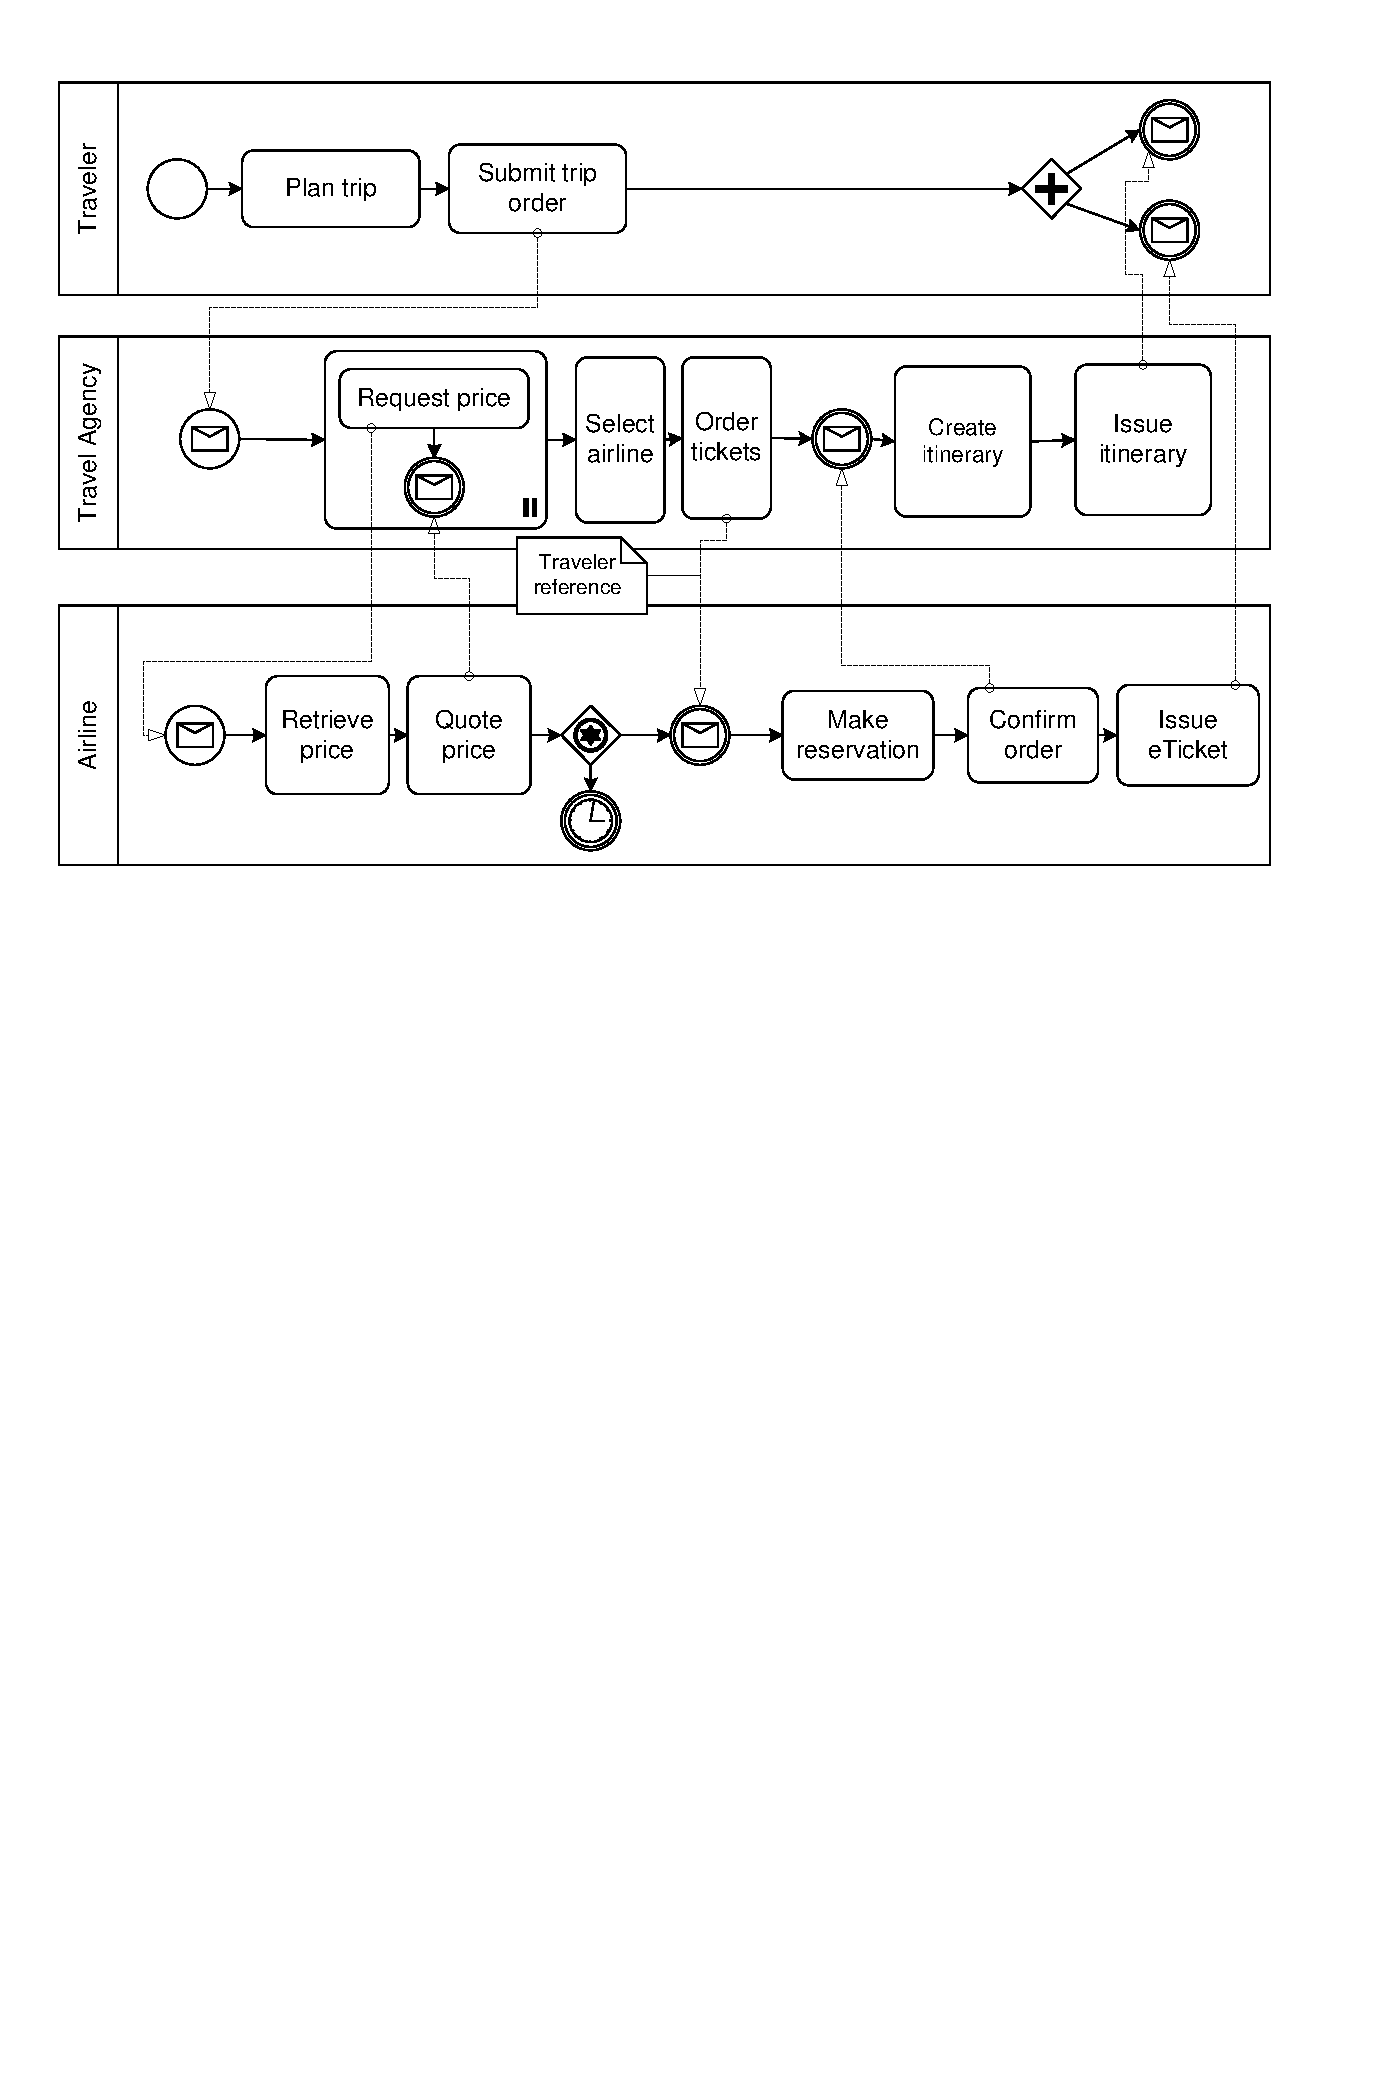
\includegraphics[width=.8\textwidth]{choreography.pdf}
    \caption[Beispiel-Choreographie]{Die Beispiel-Choreographie. Nun etwas kleiner, damit \texttt{\textbackslash textwidth} demonstriert wird. Und auch die Verwendung von alternativen Bildunterschriften für das Verzeichnis der Abbildungen. Letzteres ist allerdings nur Bedingt zu empfehlen, denn wer liesst schon so viel Text unter einem Bild? Oder ist es einfach nur Stilsache?}
    \label{fig:chor2}
  \end{center}
\end{figure}

\section{Tabellen}
Tabelle~\ref{tab:Ergebnisse} zeigt Ergebnisse.
\begin{table}
  \begin{center}
    \begin{tabular}{ccc}
	\toprule
	\multicolumn{2}{c}{\textbf{zusammengefasst}} & \textbf{Titel} \\ \midrule
	Tabelle & wie & in \\
	\url{tabsatz.pdf}& empfohlen & gesetzt\\
	
	\multirow{2}{*}{Beispiel} & \multicolumn{2}{c}{ein schönes Beispiel}\\
	 & \multicolumn{2}{c}{für die Verwendung von \gq{multirow}}\\
	\bottomrule
    \end{tabular}
    \caption[Beispieltabelle]{Beispieltabelle -- siehe \url{http://www.ctan.org/tex-archive/info/german/tabsatz/}}
    \label{tab:Ergebnisse}
  \end{center}
\end{table}

\section{Pseudocode}
Algorithmus~\vref{alg:sample} zeigt einen Beispielalgorithmus.
\begin{Algorithmus} %Die Umgebung nur benutzen, wenn man den Algorithmus ähnlich wie Graphiken von TeX platzieren lassen möchte
\caption{Sample algorithm}
\label{alg:sample}
\begin{algorithmic}
\Procedure{Sample}{$a$,$v_e$}
\State $\mathsf{parentHandled} \gets (a = \mathsf{process}) \lor \mathsf{visited}(a'), (a',c,a) \in \mathsf{HR}$ 
\State \Comment $(a',c'a) \in \mathsf{HR}$ denotes that $a'$ is the parent of $a$
\If{$\mathsf{parentHandled}\,\land(\mathcal{L}_\mathit{in}(a)=\emptyset\,\lor\,\forall l \in \mathcal{L}_\mathit{in}(a): \mathsf{visited}(l))$}
\State $\mathsf{visited}(a) \gets \text{true}$
\State $\mathsf{writes}_\circ(a,v_e) \gets
\begin{cases}
\mathsf{joinLinks}(a,v_e) & \abs{\mathcal{L}_\mathit{in}(a)} > 0\\
\mathsf{writes}_\circ(p,v_e)
& \exists p: (p,c,a) \in \mathsf{HR}\\
(\emptyset, \emptyset, \emptyset, false) & \text{otherwise}
\end{cases}
$
\If{$a\in\mathcal{A}_\mathit{basic}$}
  \State \Call{HandleBasicActivity}{$a$,$v_e$}
\ElsIf{$a\in\mathcal{A}_\mathit{flow}$}
  \State \Call{HandleFlow}{$a$,$v_e$}
\ElsIf{$a = \mathsf{process}$} \Comment Directly handle the contained activity
  \State \Call{HandleActivity}{$a'$,$v_e$}, $(a,\bot,a') \in \mathsf{HR}$
  \State $\mathsf{writes}_\bullet(a) \gets \mathsf{writes}_\bullet(a')$
\EndIf
\ForAll{$l \in \mathcal{L}_\mathit{out}(a)$}
  \State \Call{HandleLink}{$l$,$v_e$}
\EndFor
\EndIf
\EndProcedure
\end{algorithmic}
\end{Algorithmus}

\clearpage
Und wer einen Algorithmus schreiben möchte, der über mehrere Seiten geht, der kann das nur mit folgendem \textbf{üblen} Hack tun:

{
\begin{minipage}{\textwidth}
\hrule height .8pt width\textwidth
\vskip.15em%\vskip\abovecaptionskip\relax
\stepcounter{Algorithmus}
\addcontentsline{alg}{Algorithmus}{\protect\numberline{\theAlgorithmus}{\ignorespaces Description \relax}}
\noindent\textbf{Algorithmus \theAlgorithmus} Description
%\stepcounter{algorithm}
%\addcontentsline{alg}{Algorithmus}{\thealgorithm{}\hskip0em Description}
%\textbf{Algorithmus \thealgorithm} Description
\vskip.3em%\vskip\belowcaptionskip\relax
\hrule height .5pt width\textwidth
\end{minipage}
code goes here\\
test2\\
\vskip-.9em
\hrule height .5pt width\textwidth
}

\section{Verweise}
Verweise auf einen Abschnitt gehen mittels: ``Siehe Abschnitt~\vref{sec:mf}''. Das Kommando \texttt{\textbackslash{}vref} funktioniert ähnlich wie \texttt{\textbackslash{}ref} mit dem Unterschied, dass zusätzlich ein Verweis auf die Seite hinzugefügt wird. \texttt{vref}: Abschnitt \vref{sec:diff}, \texttt{ref}: \ref{sec:diff}.

%Mit MiKTeX Installationsstund 2012-01-16 nicht mehr nötig
%Falls ein Abschnitt länger als eine Seite wird und man mittels \texttt{\textbackslash{}vref} auf eine konkrete Stelle in der Section
%verweisen möchte, dann sollte man \texttt{\textbackslash{}phantomsection} verwenden und dann wird
%auch bei \texttt{vref} die richtige Seite angeben.

%%The link location will be placed on the line below.
%%Tipp von http://en.wikibooks.org/wiki/LaTeX/Labels_and_Cross-referencing#The_hyperref_package_and_.5Cphantomsection
%\phantomsection
%\label{alabel}
%Das Beispiel für \texttt{\textbackslash{}phantomsection} bitte im \LaTeX{}-Quellcode anschauen.

%Hier das Beispiel: Siehe Abschnitt \vref{hack1} und Abschnitt \vref{hack2}.

\section{Verschiedenes}
\label{sec:diff}
\ifdeutsch
Ziffern (123\,654\,789) werden schön gesetzt. Falls dies nicht gewünscht ist, den Parameter \texttt{osf} bei dem Paket \texttt{mathpazo} herausnehmen.
\fi

\textsc{Kapitälchen} werden schön gesperrt...

\begin{compactenum}[I]
\item Man kann auch die Nummerierung dank paralist kompakt halten
\item und auf eine andere Nummerierung umstellen
\end{compactenum}

\section{Weitere Informationen}
Verbesserungsvorschläge für diese Vorlage sind immer willkommen. Bitte im Trac ein Ticket eingragen (\url{https://vorlagen.studiforge.informatik.uni-stuttgart.de/trac.fcgi/wiki/WikiStart}). Vom Trac sind weitere \LaTeX-Seiten verlinkt.
%%Folgende Zeile aktivieren und als SVN property "svn:keywords" auf "Id" setzen, um SVN Versionsinformationen im Dokument zu erhalten
%\svnInfo $Id: kapitel2.tex 62 2012-04-20 15:14:01Z koppor $ 

%Die Angabe des schlauen Spruchs auf diesem Wege funtioniert nur,
%wenn keine Änderung des Kapitels mittels den in preambel/chapterheads.tex
%vorgeschlagenen Möglichkeiten durchgeführt wurde.
\chapter{SIFT/SURF}
%\vspace{-3cm}
%\vspace{2cm}

\label{chap:k3}
SIFT (Scale-invariant feature transform) ist ein von David Lowe 1999 vorgestelltes Verfahren zur Extraktion von lokalen Merkmalen aus Bildern. Die mit diesem Verfahren gefundene Merkmale haben die Eingeschaft, dass sie robust gegenüber Rotation, Translation und Skalierung sind, und damit zuverlässig in anderen Bilder wiedererkannt werden können.
Um Objekte in Bildern mit SIFT erkennen und lokalisieren zu können, sind also zwei Schritte nötig:
\begin{enumerate}
	\item Extraktion und Beschreibung von Merkmalen (Features) des gesuchten Objekts
	\item Lokalisation der Merkmale im Suchbild
\end{enumerate}

\section{Extraktion und Beschreibung von Merkmalen (Features) des gesuchten Objekts}
Der Algorithmus zur Extraktion und Beschreibung der Merkmale besteht dabei aus vier Verarbeitungsstufen:
\subsection{Ermittlung potentieller Merkmale in DoG-Pyramiden}
Um Merkmale zu ermitteln, die robust gegenüber Skalierung sind, kommt das Verfahren der DoG (Difference of gaussians) Pyramiden zum Einsatz. Dabei werden aus dem Ausgangsbild zunächst n Gaußpyramiden berechnet. Eine Pyramide besteht dabei aus fortlaufen stärker geglätteten Bildern des Ausgangsbildes $g$. Zur Glättung kommt dabei ein Gaußfilter $G$ zum Einsatz:
\begin{equation*}
 g(x, y) * G_\vartheta (x, y) = g(x, y) * (\frac{1}{\sqrt{2\pi \vartheta ^2}}\cdot e^{-\frac{x^2 + y^2}{2\vartheta ^2}})
\end{equation*}

Im Anschluss wird das letzte Bild der Pyramide um 50\% verkleinert, und daraus durch erneute fortlaufende Glättung mit dem Gaußfilter eine neue Pyramide erzeugt.
Je zwei benachbarte Bilder einer Gaußpyramide werden nun voneinander Subtrahiert. Aus den Resultaten entstehen dabei die DoG Pyramiden:
\begin{figure}
  \begin{center}
    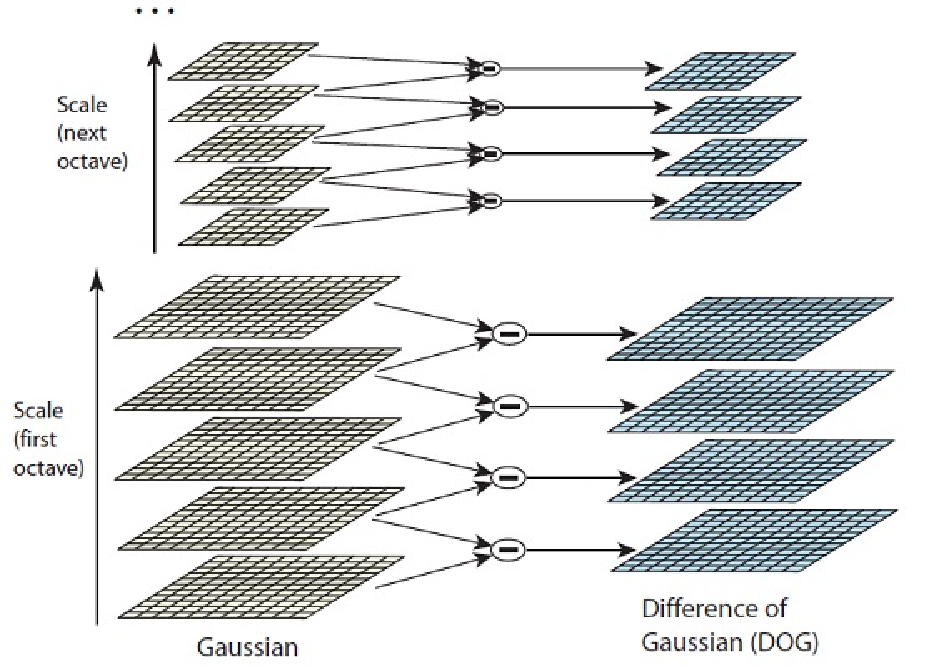
\includegraphics[width=\textwidth]{dog.pdf}
    \caption{DoG-Pyramiden}
    \label{fig:dog_pyr}
  \end{center}
\end{figure}

Die dadurch erzeugten DoG-Pyramiden werden nun auf minimale und maximale Pixelwerte untersucht.
Ein Maximum ist gefunden, wenn der Grauwert eines Pixels größer als der seiner 26 Nachbarn ist. Nachbarschaft eines Pixels ergibt sich dann aus seinen acht Nachbarn der selben Ebene, sowie aus den jeweils neun Nachbarn der benachbarten Ebenen in der DoG-Pyramide.
Die Suche nach Minima erfolg auf die selbe Art und Weise. Die Information, auf welcher Skalierung die potentiellen Merkmalspunkte liegen, wird dabei ebenfalls gespeichert.
\begin{figure}[H]
  \begin{center}
    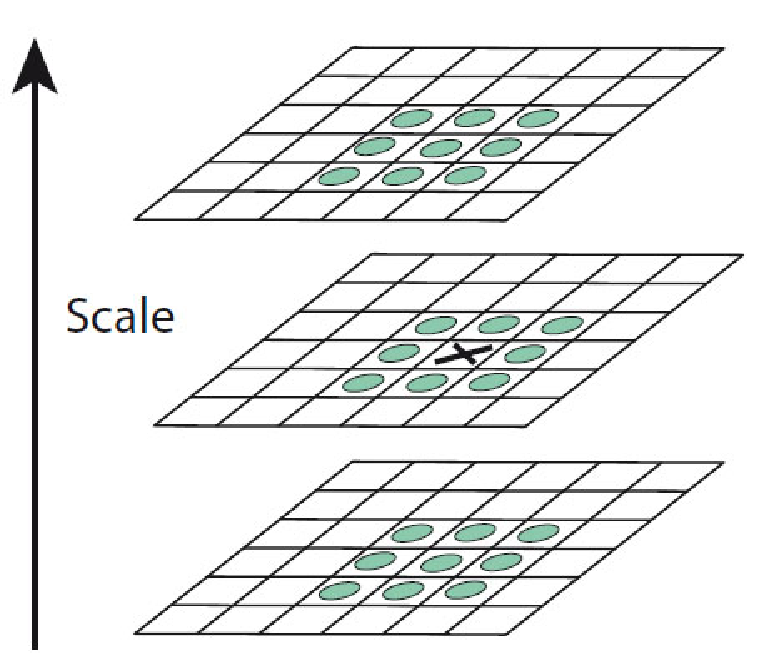
\includegraphics[width=0.5\textwidth]{scale.pdf}
    \caption{Nachbarschaft eines Pixels}
    \label{fig:neighbor}
  \end{center}
\end{figure}

\subsection{Filterung und Lokalisation potentieller Merkmalspunkte}
as oben genannte Verfahren liefert neben den robusten Merkmalspunkten eine große Menge von instabilen, für die weitere Verarbeitung nicht zu gebrauchende Merkmale.
Daher werden die gefundenen Merkmalspunkte anhand von Stabilitätskriterien gefiltert.
Im ersten Schritt werden dabei alle Merkmalspunkte entfernt, die einen DoG-Wert von weniger als 0,03, und somit einen relativ niedrigen Kontrast besitzen.
Merkmalspunkte, die auf Ecken liegen sind “prägnanter” (und somit staibler) als solche, die auf einer Kante liegen, daher werden alle Merkmalspunkte entfernt, die auf einer Kante, aber nicht auf einer Ecke liegen.
Dies geschieht unter Anwendung der Hesse-Matrix (todo).

\subsection{Bestimmung der Hauptorientierungen}
Um Invarianz der verbleibenden Merkmalspunkte gegenüber Rotation zu erreichen, wird für jeden Merkmalspunkt dessen Hauptorientierung berechnet.
Dafür nutzt man das gaußgefilterte Bild, welches der Skalierung des zu untersuchenden Merkmalspunktes am nächsten kommt. In diesem Bild werden nun innerhalb einer festen Region um den Merkmalspunkt herum die Gradientenlängen $m(x, y)$ und die Gradientenorientierungen $\theta (x, y)$ bezüglich eines Punktes $g(x, y)$ berechnet, wobei
\begin{equation*}
m(x, y) = \sqrt{(g(x + 1, y) - g(x - 1, y))^2 +(g(x, y+1) - g(x, y-1))^2}
\end{equation*}

und

\begin{equation*}
\theta (x, y) = tan^{-1}\cdot \frac{g(x +1, y) - g(x-1, y)}{g(x, y +1) - g(x, y-1)}
\end{equation*}

Die so ermittelten Gradientenorientierungen werden nun anhand ihrer Gradientenlängen gewichtet. Dadurch haben Gradientenrichtungen mit großer Gradientenlänge einen größeren Einfluss auf die Hauptorientierung als Gradientenrichtungen mit niedriger Gradientenlänge.
Danach werden die Gradientenorientierungen zusätzlich anhand ihrer Entfernung zum Merkmalspunkt gewichtet, um Gradientenrichtungen, die sich näher am Merkmalspunkt befinden stärker zu gewichten.

Aus den gewichteten Gradientenorientierungen wird nun ein Orientierungshistogramm erstellt. Dieses Histogramm ist in 36 Winkelbereiche eingeteilt und hat somit eine Klassenbreite von $10\,^{\circ}$.
Jede Gradientenorientierung wird dabei anhand ihrer Gewichtung an der passenden Stelle im Histogramm aufaddiert. \\
Nach der Erstellung des Histogramms kann aus diesem die Gradientenlänge $m_{max}$ abgelesen werden (Winkelbereich mit der größten Summe). Die Hauptorientierung des Merkmalspunktes  setzt sich dabei aus $m_{max}$, sowie der zugehörigen Gradientenorientierung $\theta_{max}$ maxzusammen.
Für den Fall, dass eine weitere Orientierung mit der Gradientenlänge $m_i > 0,8 m_{max}$
existiert; wie es bei Eckpunkten häufig der Fall ist; wird an der Stelle $(x, y)$ ein weiterer Merkmalspunkt mit der Hauptorientierung $(m_i, \theta_i)$ erstellt.

\section{Lokalisation der Merkmale im Suchbild}
\label{sec:mf}
Mathematische Formeln kann man $so$ setzen. \texttt{symbols-a4.pdf} (zu finden auf \url{http://www.ctan.org/tex-archive/info/symbols/comprehensive/symbols-a4.pdf}) enthält eine Liste der unter LaTeX direkt verfügbaren Symbole. z.\,B.\ $\mathbb{N}$ für die Menge der natürlichen Zahlen. Für eine vollständige Dokumentation für mathematischen Formelsatz sollte die Dokumentation zu \texttt{amsmath}, \url{ftp://ftp.ams.org/pub/tex/doc/amsmath/} gelesen werden.

Folgende Gleichung erhält keine Nummer, da \texttt{\textbackslash equation*} verwendet wurde.

\begin{equation*}
x = y
\end{equation*}

Die Gleichung~\ref{eq:test} erhält eine Nummer:
\begin{equation}
\label{eq:test}
x = y
\end{equation}

Eine ausführliche Anleitung zum Mathematikmodus von LaTeX findet sich in \url{http://www.ctan.org/tex-archive/help/Catalogue/entries/voss-mathmode.html}.

\section{Quellcode}
Listing~\ref{lst:ListingANDlstlisting} zeigt, wie man Programmlistings einbindet.  Mittels \texttt{\textbackslash lstinputlisting} kann man den Inhalt direkt aus Dateien lesen.

%Listing-Umgebung wurde durch \newfloat{Listing} definiert
\begin{Listing}
\begin{lstlisting}
<listing name="second sample">
  <content>not interesting</content>
</listing>
\end{lstlisting}
\caption{lstlisting in einer Listings-Umgebung, damit das Listing durch Balken abgetrennt ist}
\label{lst:ListingANDlstlisting}
\end{Listing}

Quellcode im \lstinline|<listing />| ist auch möglich.

\section{Abbildungen}
Die Abbildungen~\ref{fig:chor1} und~\ref{fig:chor2} sind für das Verständnis dieses Dokuments
wichtig. Im Anhang zeigt Abbildung~\vref{fig:AnhangsChor} erneut die komplette Choreographie.

%Die Parameter in eckigen Klammern sind optionale Parameter - z.B. [htb!]
%htb! bedeutet: "Liebes LaTeX, bitte platziere diese Abbildung zuerst hier ("_h_ere"). Falls das nicht funktioniert, dann bitte oben auf der Seite ("_t_op"). Und falls das nicht geht, bitte unten auf der Seite ("_b_ottom"). Und bitte, bitte bevorzuge hier und oben, auch wenn's net so optimal aussieht ("!")
%Diese sollten nach Möglichkeit NICHT verwendet werden. LaTeX's Algorithmus für das Platzieren der Gleitumgebung ist schon sehr gut!
\begin{figure}
  \begin{center}
    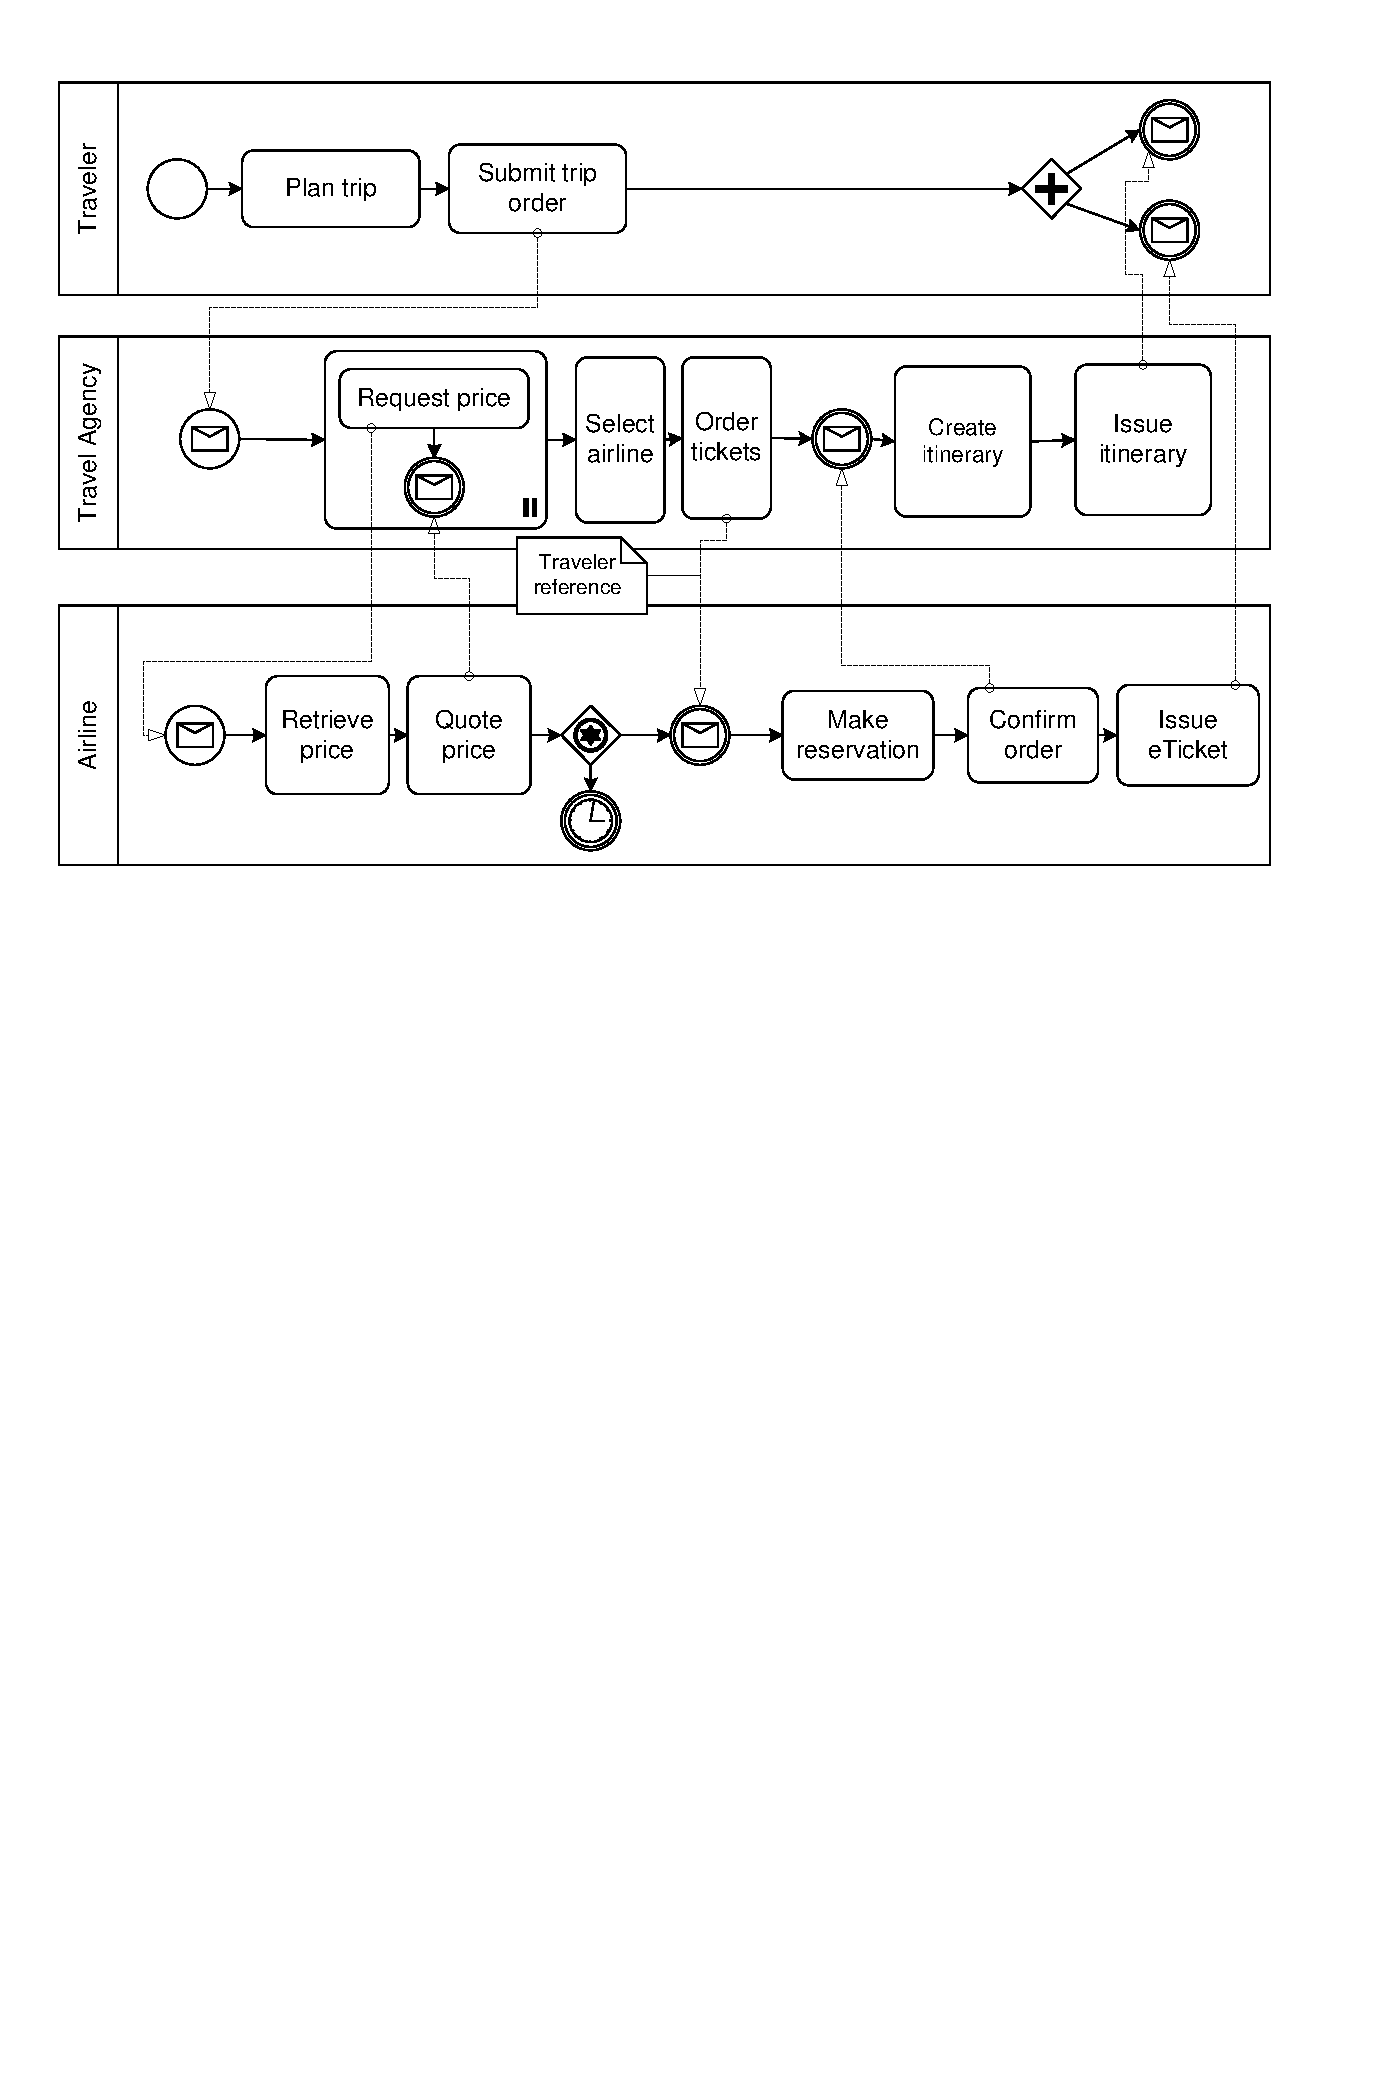
\includegraphics[width=\textwidth]{choreography.pdf}
    \caption{Beispiel-Choreographie}
    \label{fig:chor1}
  \end{center}
\end{figure}

\begin{figure}
  \begin{center}
    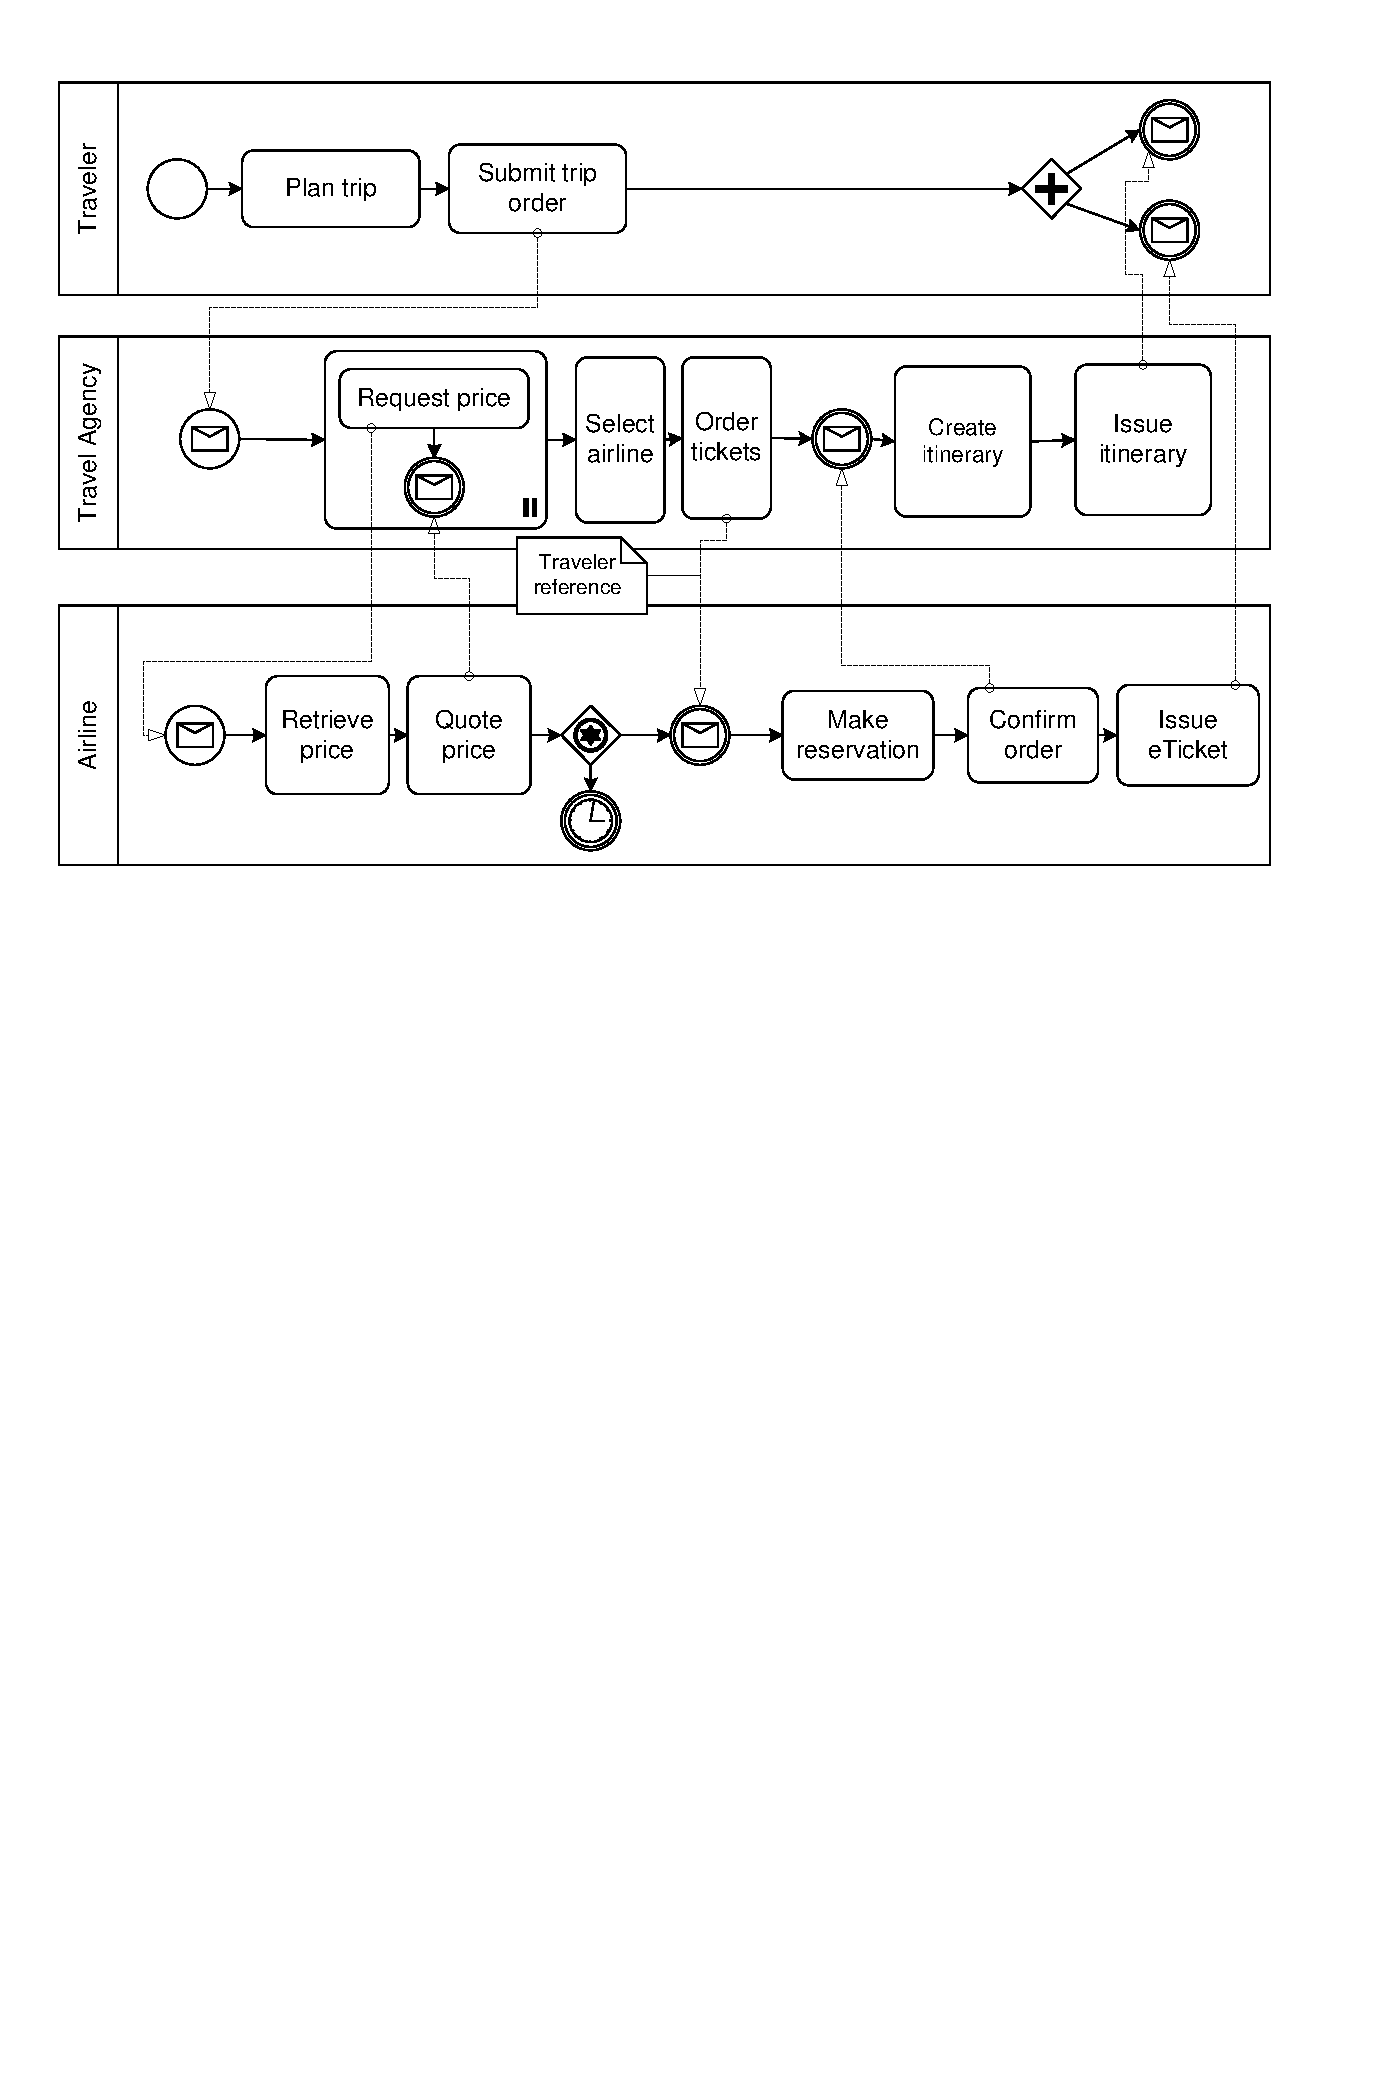
\includegraphics[width=.8\textwidth]{choreography.pdf}
    \caption[Beispiel-Choreographie]{Die Beispiel-Choreographie. Nun etwas kleiner, damit \texttt{\textbackslash textwidth} demonstriert wird. Und auch die Verwendung von alternativen Bildunterschriften für das Verzeichnis der Abbildungen. Letzteres ist allerdings nur Bedingt zu empfehlen, denn wer liesst schon so viel Text unter einem Bild? Oder ist es einfach nur Stilsache?}
    \label{fig:chor2}
  \end{center}
\end{figure}

\section{Tabellen}
Tabelle~\ref{tab:Ergebnisse} zeigt Ergebnisse.
\begin{table}
  \begin{center}
    \begin{tabular}{ccc}
	\toprule
	\multicolumn{2}{c}{\textbf{zusammengefasst}} & \textbf{Titel} \\ \midrule
	Tabelle & wie & in \\
	\url{tabsatz.pdf}& empfohlen & gesetzt\\
	
	\multirow{2}{*}{Beispiel} & \multicolumn{2}{c}{ein schönes Beispiel}\\
	 & \multicolumn{2}{c}{für die Verwendung von \gq{multirow}}\\
	\bottomrule
    \end{tabular}
    \caption[Beispieltabelle]{Beispieltabelle -- siehe \url{http://www.ctan.org/tex-archive/info/german/tabsatz/}}
    \label{tab:Ergebnisse}
  \end{center}
\end{table}

\section{Pseudocode}
Algorithmus~\vref{alg:sample} zeigt einen Beispielalgorithmus.
\begin{Algorithmus} %Die Umgebung nur benutzen, wenn man den Algorithmus ähnlich wie Graphiken von TeX platzieren lassen möchte
\caption{Sample algorithm}
\label{alg:sample}
\begin{algorithmic}
\Procedure{Sample}{$a$,$v_e$}
\State $\mathsf{parentHandled} \gets (a = \mathsf{process}) \lor \mathsf{visited}(a'), (a',c,a) \in \mathsf{HR}$ 
\State \Comment $(a',c'a) \in \mathsf{HR}$ denotes that $a'$ is the parent of $a$
\If{$\mathsf{parentHandled}\,\land(\mathcal{L}_\mathit{in}(a)=\emptyset\,\lor\,\forall l \in \mathcal{L}_\mathit{in}(a): \mathsf{visited}(l))$}
\State $\mathsf{visited}(a) \gets \text{true}$
\State $\mathsf{writes}_\circ(a,v_e) \gets
\begin{cases}
\mathsf{joinLinks}(a,v_e) & \abs{\mathcal{L}_\mathit{in}(a)} > 0\\
\mathsf{writes}_\circ(p,v_e)
& \exists p: (p,c,a) \in \mathsf{HR}\\
(\emptyset, \emptyset, \emptyset, false) & \text{otherwise}
\end{cases}
$
\If{$a\in\mathcal{A}_\mathit{basic}$}
  \State \Call{HandleBasicActivity}{$a$,$v_e$}
\ElsIf{$a\in\mathcal{A}_\mathit{flow}$}
  \State \Call{HandleFlow}{$a$,$v_e$}
\ElsIf{$a = \mathsf{process}$} \Comment Directly handle the contained activity
  \State \Call{HandleActivity}{$a'$,$v_e$}, $(a,\bot,a') \in \mathsf{HR}$
  \State $\mathsf{writes}_\bullet(a) \gets \mathsf{writes}_\bullet(a')$
\EndIf
\ForAll{$l \in \mathcal{L}_\mathit{out}(a)$}
  \State \Call{HandleLink}{$l$,$v_e$}
\EndFor
\EndIf
\EndProcedure
\end{algorithmic}
\end{Algorithmus}

\clearpage
Und wer einen Algorithmus schreiben möchte, der über mehrere Seiten geht, der kann das nur mit folgendem \textbf{üblen} Hack tun:

{
\begin{minipage}{\textwidth}
\hrule height .8pt width\textwidth
\vskip.15em%\vskip\abovecaptionskip\relax
\stepcounter{Algorithmus}
\addcontentsline{alg}{Algorithmus}{\protect\numberline{\theAlgorithmus}{\ignorespaces Description \relax}}
\noindent\textbf{Algorithmus \theAlgorithmus} Description
%\stepcounter{algorithm}
%\addcontentsline{alg}{Algorithmus}{\thealgorithm{}\hskip0em Description}
%\textbf{Algorithmus \thealgorithm} Description
\vskip.3em%\vskip\belowcaptionskip\relax
\hrule height .5pt width\textwidth
\end{minipage}
code goes here\\
test2\\
\vskip-.9em
\hrule height .5pt width\textwidth
}

\section{Verweise}
Verweise auf einen Abschnitt gehen mittels: ``Siehe Abschnitt~\vref{sec:mf}''. Das Kommando \texttt{\textbackslash{}vref} funktioniert ähnlich wie \texttt{\textbackslash{}ref} mit dem Unterschied, dass zusätzlich ein Verweis auf die Seite hinzugefügt wird. \texttt{vref}: Abschnitt \vref{sec:diff}, \texttt{ref}: \ref{sec:diff}.

%Mit MiKTeX Installationsstund 2012-01-16 nicht mehr nötig
%Falls ein Abschnitt länger als eine Seite wird und man mittels \texttt{\textbackslash{}vref} auf eine konkrete Stelle in der Section
%verweisen möchte, dann sollte man \texttt{\textbackslash{}phantomsection} verwenden und dann wird
%auch bei \texttt{vref} die richtige Seite angeben.

%%The link location will be placed on the line below.
%%Tipp von http://en.wikibooks.org/wiki/LaTeX/Labels_and_Cross-referencing#The_hyperref_package_and_.5Cphantomsection
%\phantomsection
%\label{alabel}
%Das Beispiel für \texttt{\textbackslash{}phantomsection} bitte im \LaTeX{}-Quellcode anschauen.

%Hier das Beispiel: Siehe Abschnitt \vref{hack1} und Abschnitt \vref{hack2}.

\section{Verschiedenes}
\label{sec:diff}
\ifdeutsch
Ziffern (123\,654\,789) werden schön gesetzt. Falls dies nicht gewünscht ist, den Parameter \texttt{osf} bei dem Paket \texttt{mathpazo} herausnehmen.
\fi

\textsc{Kapitälchen} werden schön gesperrt...

\begin{compactenum}[I]
\item Man kann auch die Nummerierung dank paralist kompakt halten
\item und auf eine andere Nummerierung umstellen
\end{compactenum}

\section{Weitere Informationen}
Verbesserungsvorschläge für diese Vorlage sind immer willkommen. Bitte im Trac ein Ticket eingragen (\url{https://vorlagen.studiforge.informatik.uni-stuttgart.de/trac.fcgi/wiki/WikiStart}). Vom Trac sind weitere \LaTeX-Seiten verlinkt.
%Folgende Zeile aktivieren und als SVN property "svn:keywords" auf "Id" setzen, um SVN Versionsinformationen im Dokument zu erhalten
%\svnInfo $Id: zusammenfassung_und_ausblick.tex 60 2012-01-26 15:56:06Z koppor $ 

\chapter{Zusammenfassung und Ausblick}\label{chap:zusfas}
Hier bitte einen kurzen Durchgang durch die Arbeit.

\section*{Ausblick}
...und anschließend einen Ausblick


%
%
%\renewcommand{\appendixtocname}{Anhang}
%\renewcommand{\appendixname}{Anhang}
%\renewcommand{\appendixpagename}{Anhang}
\appendix
%Folgende Zeile aktivieren und als SVN property "svn:keywords" auf "Id" setzen, um SVN Versionsinformationen im Dokument zu erhalten
%\svnInfo $Id: anhang.tex 62 2012-04-20 15:14:01Z koppor $ 

\chapter{Ein Anhang}
...falls gewünscht...

Und hier noch ein Text aus dem Projekt Gutenberg zum Test der Ränder und des optischen Randausgleichs

Des Lebens Überfluss\footnote{\url{http://gutenberg.spiegel.de/tieck/ueberflu/ueberflu.htm}}.
von Ludwig Tieck.

In einem der härtesten Winter war gegen Ende des Februar ein sonderbarer Tumult gewesen, über dessen Entstehung, Fortgang und Beruhigung die seltsamsten und widersprechendsten Gerüchte in der Residenz umliefen. Es ist natürlich, dass, wenn alle Menschen sprechen und erzählen wollen, ohne den Gegenstand ihrer Darstellung zu kennen, auch das Gewöhnliche die Farbe der Fabel annimmt.

In der Vorstadt, die ziemlich bevölkert ist hatte sich in einer der engsten Straßen das Abenteuer zugetragen. Bald hieß es, ein Verräter und Rebell sei entdeckt und von der Polizei aufgehoben worden, bald, ein Gottesleugner, der mit andern Atheisten verbrüdert das Christentum mit seiner Wurzel ausrotten wollen, habe sich nach hartnäckigem Widerstand den Behörden ergeben und sitze nun so lange fest, bis er in der Einsamkeit bessere Grundsätze und Überzeugungen finde. Er habe sich aber vorher noch in seiner Wohnung mit alten Doppelhaken, ja sogar mit einer Kanone verteidigt, und es sei, bevor er sich ergeben, Blut geflossen, so dass das Konsistorium wie das Kriminalgericht wohl auf seine Hinrichtung antragen werde. Ein politischer Schuhmacher wollte wissen, der Verhaftete sei ein Emissär, der als das Haupt vieler geheimen Gesellschaften mit allen Revolutionsmännern Europas in innigster Verbindung stehe; er habe alle Fäden in Paris, London und Spanien wie in den östlichen Provinzen gelenkt, und es sei nahe daran, dass im äußersten Indien eine ungeheure Empörung ausbrechen und sich dann gleich Cholera nach Europa herüberwälzen werde, um allen Brennstoff in lichte Flammen zu setzen.

So viel war ausgemacht, in einem kleinen Hause hatte es Tumult gegeben, die Polizei war herbeigerufen worden, das Volk hatte gelärmt, angesehene Männer wurden bemerkt, die sich darein mischten, und nach einiger zeit war alles wieder ruhig, ohne dass man den Zusammenhang begriff. Im Hause selbst war eine gewisse Zerstörung nicht zu verkennen. Jeder legte sich die Sache aus, wie Laune oder Phantasie sie ihm erklären mochten. Die Zimmerleute und Tischler besserten nachher den Schaden aus.

Ein Mann hatte in diesem Hause gewohnt, den niemand in der Nachbarschaft kannte. War er ein Gelehrter? ein Politiker? ein Einheimischer? ein Fremder? Darüber wusste keiner, selbst der Klügste nicht, einen genügenden Bescheid zu geben.

Soviel ist gewiss, dieser unbekannte Mann lebte sehr still und eingezogen, man sah ihn auf keinem Spaziergange, an keinem öffentlichen Orte. Er war noch nicht alt, wohlgebildet, und seine junge Frau, die sich mit ihm dieser Einsamkeit ergeben hatte, durfte man eine Schönheit nennen.

Um Weihnachten war es, als dieser jugendliche Mann in seinem Stübchen, dicht am Ofen sitzend, also zu seiner Frau redete: »Du weißt, liebste Klara, wie sehr ich den Siebenkäs unsers Jean Paul liebe und verehre; wie dieser sein Humorist sich aber helfen würde, wenn er in unsrer Lage wäre, bleibt mir doch ein Rätsel. Nicht wahr, Liebchen, jetzt sind, so scheint es, alle Mittel erschöpft?«

»Gewiss, Heinrich«, antwortete sie lächelnd und zugleich seufzend; »wenn du aber froh und heiter bleibst, liebster aller Menschen, so kann ich mich in deiner Nähe nicht unglücklich fühlen.«

»Unglück und Glück sind nur leere Worte«, antwortete Heinrich; »als du mir aus dem Hause deiner Eltern folgtest, als du so großmütig um meinetwillen alle Rücksichten fahren ließest: da war unser Schicksal auf unsre Lebenszeit bestimmt. Lieben und leben hieß nun unsre Losung; wie wir leben würden, durfte uns ganz gleichgültig sein. Und so möchte ich noch jetzt aus starkem Herzen fragen: Wer in ganz Europa ist wohl so glücklich, als ich mich mit vollem Recht aus der ganzen Kraft meines Gefühles nennen darf?«

»Wir entbehren fast alles«, sagte sie, »nur uns selbst nicht, und ich wusste ja, als ich den Bund mit dir schloss, dass du nicht reich warst; dir war es nicht unbekannt, dass ich aus meinem väterlichen Hause nichts mit mir nehmen konnte. So ist die Armut mit unsrer Liebe eins geworden, und dieses Stübchen, unser Gespräch, unser Anblicken und Schauen in des Geliebten Auge ist unser Leben.«

»Richtig!« rief Heinrich aus und sprang auf in seiner Freude, um die Schöne lebhaft zu umarmen; »wie gestört, ewig getrennt, einsam und zerstreut wären wir nun in jenem Schwarm der vornehmen Zirkel, wenn alles in seiner Ordnung vor sich gegangen wäre. Welch Blicken, Sprechen, Handgeben, Denken dort! Man könnte sich Tiere oder selbst Marionetten so abrichten und eindrechseln, dass sie eben die Komplimente machten und solche Redensarten von sich gäben. So sind wir, mein Schatz, wie Adam und Eva hier in unserm Paradiese, und kein Engel kommt auf den ganz überflüssigen Einfall, uns daraus zu vertreiben.«

»Nur«, sagte sie etwas kleinlaut, »fängt das Holz an, ganz einzugehen, und dieser Winter ist der härteste, den ich bis jetzt noch erlebt habe.«

Heinrich lachte. »Sieh«, rief er, »ich muss aus purer Bosheit lachen, aber es ist darum noch nicht das Lachen der Verzweiflung, sondern einer gewissen Verlegenheit, da ich durchaus nicht weiß, wo ich Geld hernehmen könnte. Aber finden müssen sich die Mittel; denn es ist undenkbar, dass wir erfrieren sollten, bei so heißer Liebe, bei so warmem Blut! Pur unmöglich!«

Sie lachte ihn freundlich an und erwiderte: »Wenn ich nur so wie Lenette Kleider zum Verkaufe mitgebracht, oder überflüssige Messingkannen und Mörser oder kupferne Kessel in unsrer kleinen Wirtschaft umherständen, so wäre leicht Rat zu finden.«

»Jawohl«, sprach er mit übermütigem Ton, »wenn wir Millionärs wären, wie jener Siebenkäs, dann wäre es keine Kunst, Holz anzuschaffen und selbst bessere Nahrung.«

Sie sah im Ofen nach, in welchem Brot in Wasser kochte, um so das kärglichste Mittagsmahl herzustellen, welches dann mit einem Nachtisch von weniger Butter beschlossen werden sollte. »Während du«, sagte Heinrich, »die Aufsicht über unsre Küche führst und dem Koch die nötigen Befehle erteilst, werde ich mich zu meinen Studien niedersetzen. Wie gern schriebe ich wieder, wenn mir nicht Tinte, Papier und Feder völlig ausgegangen wären; ich möchte auch wieder einmal etwas lesen, was es auch sei, wenn ich nur noch ein Buch hätte.«

»Du musst denken, Liebster«, sagte Klara und sah schalkhaft zu ihm hinüber; »die Gedanken sind dir hoffentlich noch nicht ausgegangen.«

»Liebste Ehefrau«, erwiderte er, »unsre Wirtschaft ist so weitläuftig und groß, dass sie wohl deine ganze Aufmerksamkeit in Anspruch nimmt; zerstreue dich ja nicht, damit nicht unsre ökonomischen Verhältnisse in Verwirrung geraten. Und da ich mich jetzt in meine Bibliothek begebe, so lass mich vor jetzt in Ruhe; denn ich muss meine Kenntnisse erweitern und meinem Geiste Nahrung gönnen.«

»Er ist einzig!« sagte die Frau zu sich selber und lachte fröhlich; »und wie schön er ist!«

»So lese ich denn wieder in meinem Tagebuche«, sprach Heinrich, »das ich ehemals anlegte, und es interessiert mich, rückwärts zu studieren, mit dem Ende anzufangen und mich so nach und nach zu dem Anfange vorzubereiten, damit ich diesen um so besser verstehe. Immer muss alles echte Wissen, alles Kunstwerk und gründliche Denken in einen Kreis zusammenschlagen und Anfang und Ende innigst vereinigen, wie die Schlange, die sich in den Schwanz beißt – ein Sinnbild der Ewigkeit, wie andre sagen; ein Symbol des Verstandes und alles Richtigen, wie ich behaupte.«

Er las auf der letzten Seite, aber nur halblaut: »Man hat ein Märchen, dass ein wütender Verbrecher, zum Hungertode verdammt, sich selber nach und nach aufspeiset; im Grunde ist das nur die Fabel des Lebens und eines jeden Menschen. Dort blieb am Ende nur der Magen und das Gebiss übrig, bei uns bleibt die Seele, wie sie das Unbegreifliche nennen. Ich aber habe mich abgestreift und abgelebt. Es war beinah lächerlich, dass ich noch einen Frack nebst Zubehör besaß, da ich niemals ausgehe. Am Geburtstage meiner Frau werde ich in Weste und Hemdärmeln vor ihr erscheinen, da es doch unschicklich wäre, bei hoffährigen Leuten in einem ziemlich abgetragenen Überrock Cour zu machen.«

»Hier geht die Seite und das Buch zu Ende«, sagte Heinrich. »Alle Welt sieht ein, dass unsre Fracks eine dumme und geschmacklose Kleidung sind, alle schelten diese Uniform, aber keiner macht, so wie ich, Ernst damit, den Plunder ganz abzuschaffen. Ich erfahre nun nicht einmal aus den Zeitungen, ob andere Denkende meinem kühnen Beispiele und Vorgange folgen werden.«

Er schlug um und las die vorige Seite: »Man kann auch ohne Servietten leben. Wenn ich bedenke, wie unsre Lebensweise immer mehr und mehr in Surrogat, Stellvertretung und Lückenbüßerei übergegangen ist, so bekomme ich einen rechten Hass auf unser geiziges und knickerndes Jahrhundert und fasse, da ich es ja haben kann, den Entschluss, in der Weise unsrer viel freigebigern Altvordern zu leben. Diese elenden Servietten sind ja, was selbst die heutigen Engländer noch wissen und verachten, offenbar nur erfunden, um das Tischtuch zu schonen. Ist es also Großmut, das Tischtuch nicht zu achten, so gehe ich darin noch weiter, das Tafeltuch zusamt den Servietten für überflüssig zu erklären. Beides wird verkauft, um vom saubern Tische selbst zu essen, nach Weise er Patriarchen, nach Art der – nun? welcher Völker? Gleichviel! Essen doch viele Menschen selbst ohne Tisch. Und, wie gesagt, ich treibe dergleichen nicht aus zynischer Sparsamkeit, nach Art des Diogenes, aus dem Hause, sondern im Gegenteil im Gefühl meines Wohlstandes, um nur nicht, wie die jetzige Zeit, aus törichtem Sparen zum Verschwender zu werden.«

»Du hast es getroffen«, sagte die Gattin lächeln; »aber damals lebten wir von dem Erlös dieser überflüssigen Sachen doch noch verschwenderisch. Oft sogar hatten wir zwei Schüsseln.«

Jetzt setzten sich die beiden Gatten zum dürftigsten Mahle nieder. Wer sie gesehen, hätte sie für beneidenswerte halten müssen, so fröhlich, ja ausgelassen waren sie an der einfachen Tafel. Als die Brotsuppe verzehrt war holte Klara mit schalkhafter Miene einen verdeckten Teller aus dem Ofen und setzte dem überraschten Gatten noch einige Kartoffeln vor. »Sieh!« rief dieser, »das heißt einem, wenn man sich an den vielen Büchern satt studiert hat, eine heimliche Freude machen! Dieser gute Erdapfel hat mit zu der großen Umwälzung von Europa beigetragen. Der Held Walter Raleigh soll leben!« – Sie stießen mit den Wassergläsern an, und Heinrich sah nach, ob der Enthusiasmus auch nicht einen Riss im Glase verursacht habe. »Um diese ungeheure Künstlichkeit«, sagte er dann, »um diese Einrichtung mit unsern alltäglichen Gläsern würden uns die reichsten Fürsten des Altertums beneidet haben. Es muss langweilig sein, aus einem goldenen Pokal zu trinken, vollends so schönes, klares, gesundes Wasser. Aber in unsern Gläsern schwebt die erfrischende Welle so heiter durchsichtig, so eins mit dem Becher, dass man wirklich versucht wird, zu glauben, man genieße den flüssig gewordenen Äther selbst. – Unsre Mahlzeit ist geschlossen; umarmen wir uns.«

\section{Weitere Illustrationen}
Abbildungen~\ref{fig:AnhangsChor} und~\ref{fig:AnhangsChor2} zeigen zwei Choreographien, die den
Sachverhalt weiter erläutern sollen. Die zweite Abbildung ist um 90 Grad gedreht, um das Paket
\texttt{rotating} zu demonstrieren.

\begin{figure}
  \begin{center}
    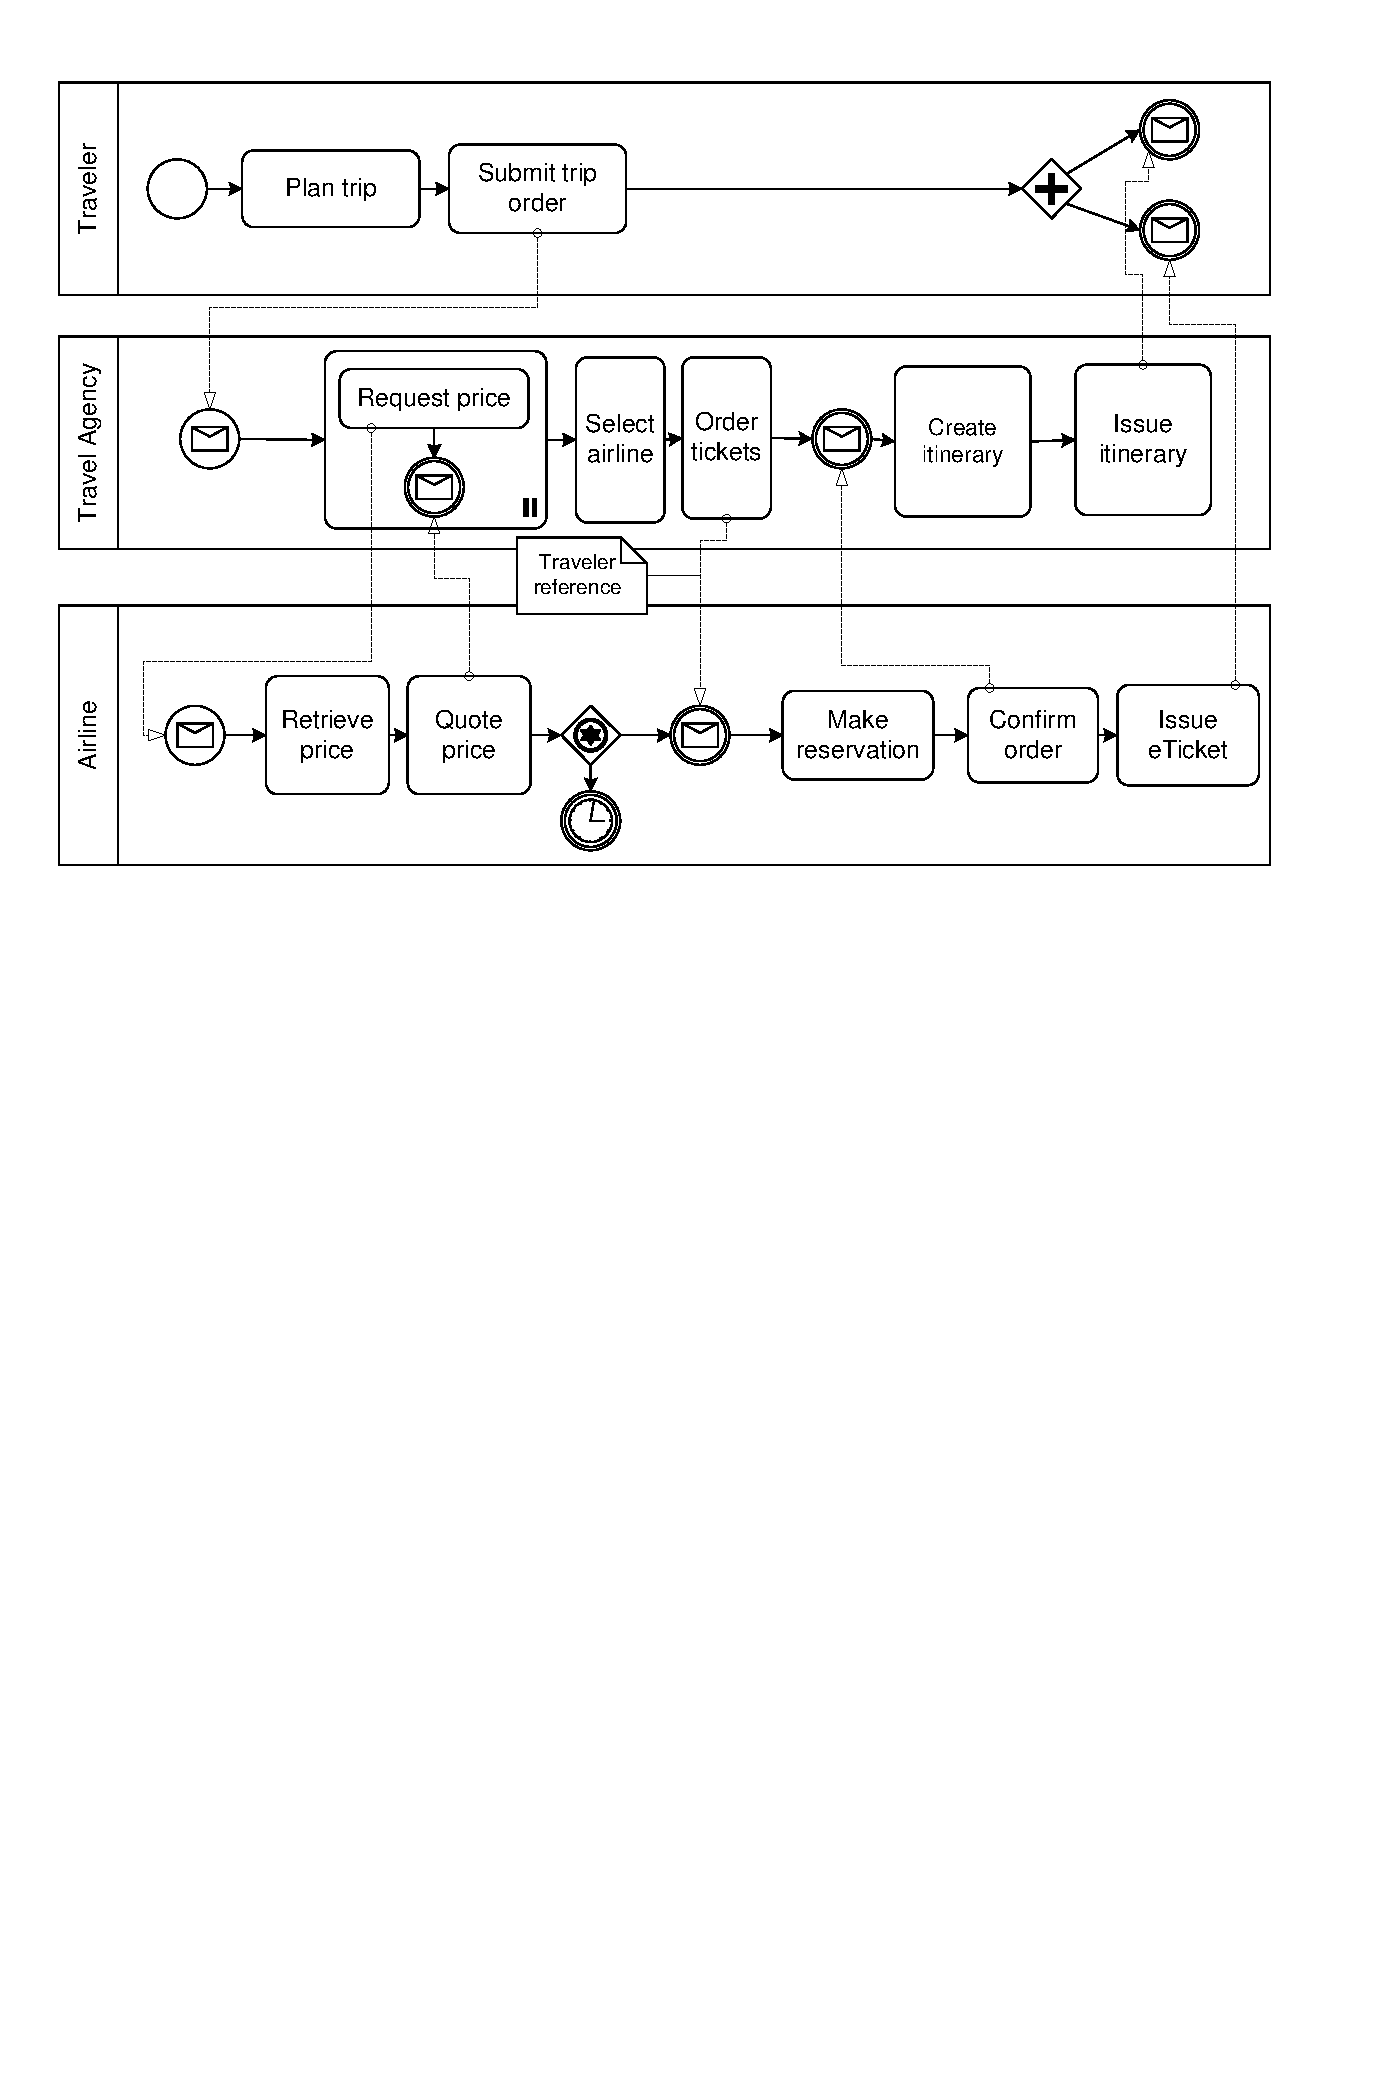
\includegraphics[width=\textwidth]{choreography.pdf}
    \caption{Beispiel-Choreographie I}
    \label{fig:AnhangsChor}
  \end{center}
\end{figure}

\begin{landscape}
%sidewaysfigure
\begin{figure}
  \begin{center}
    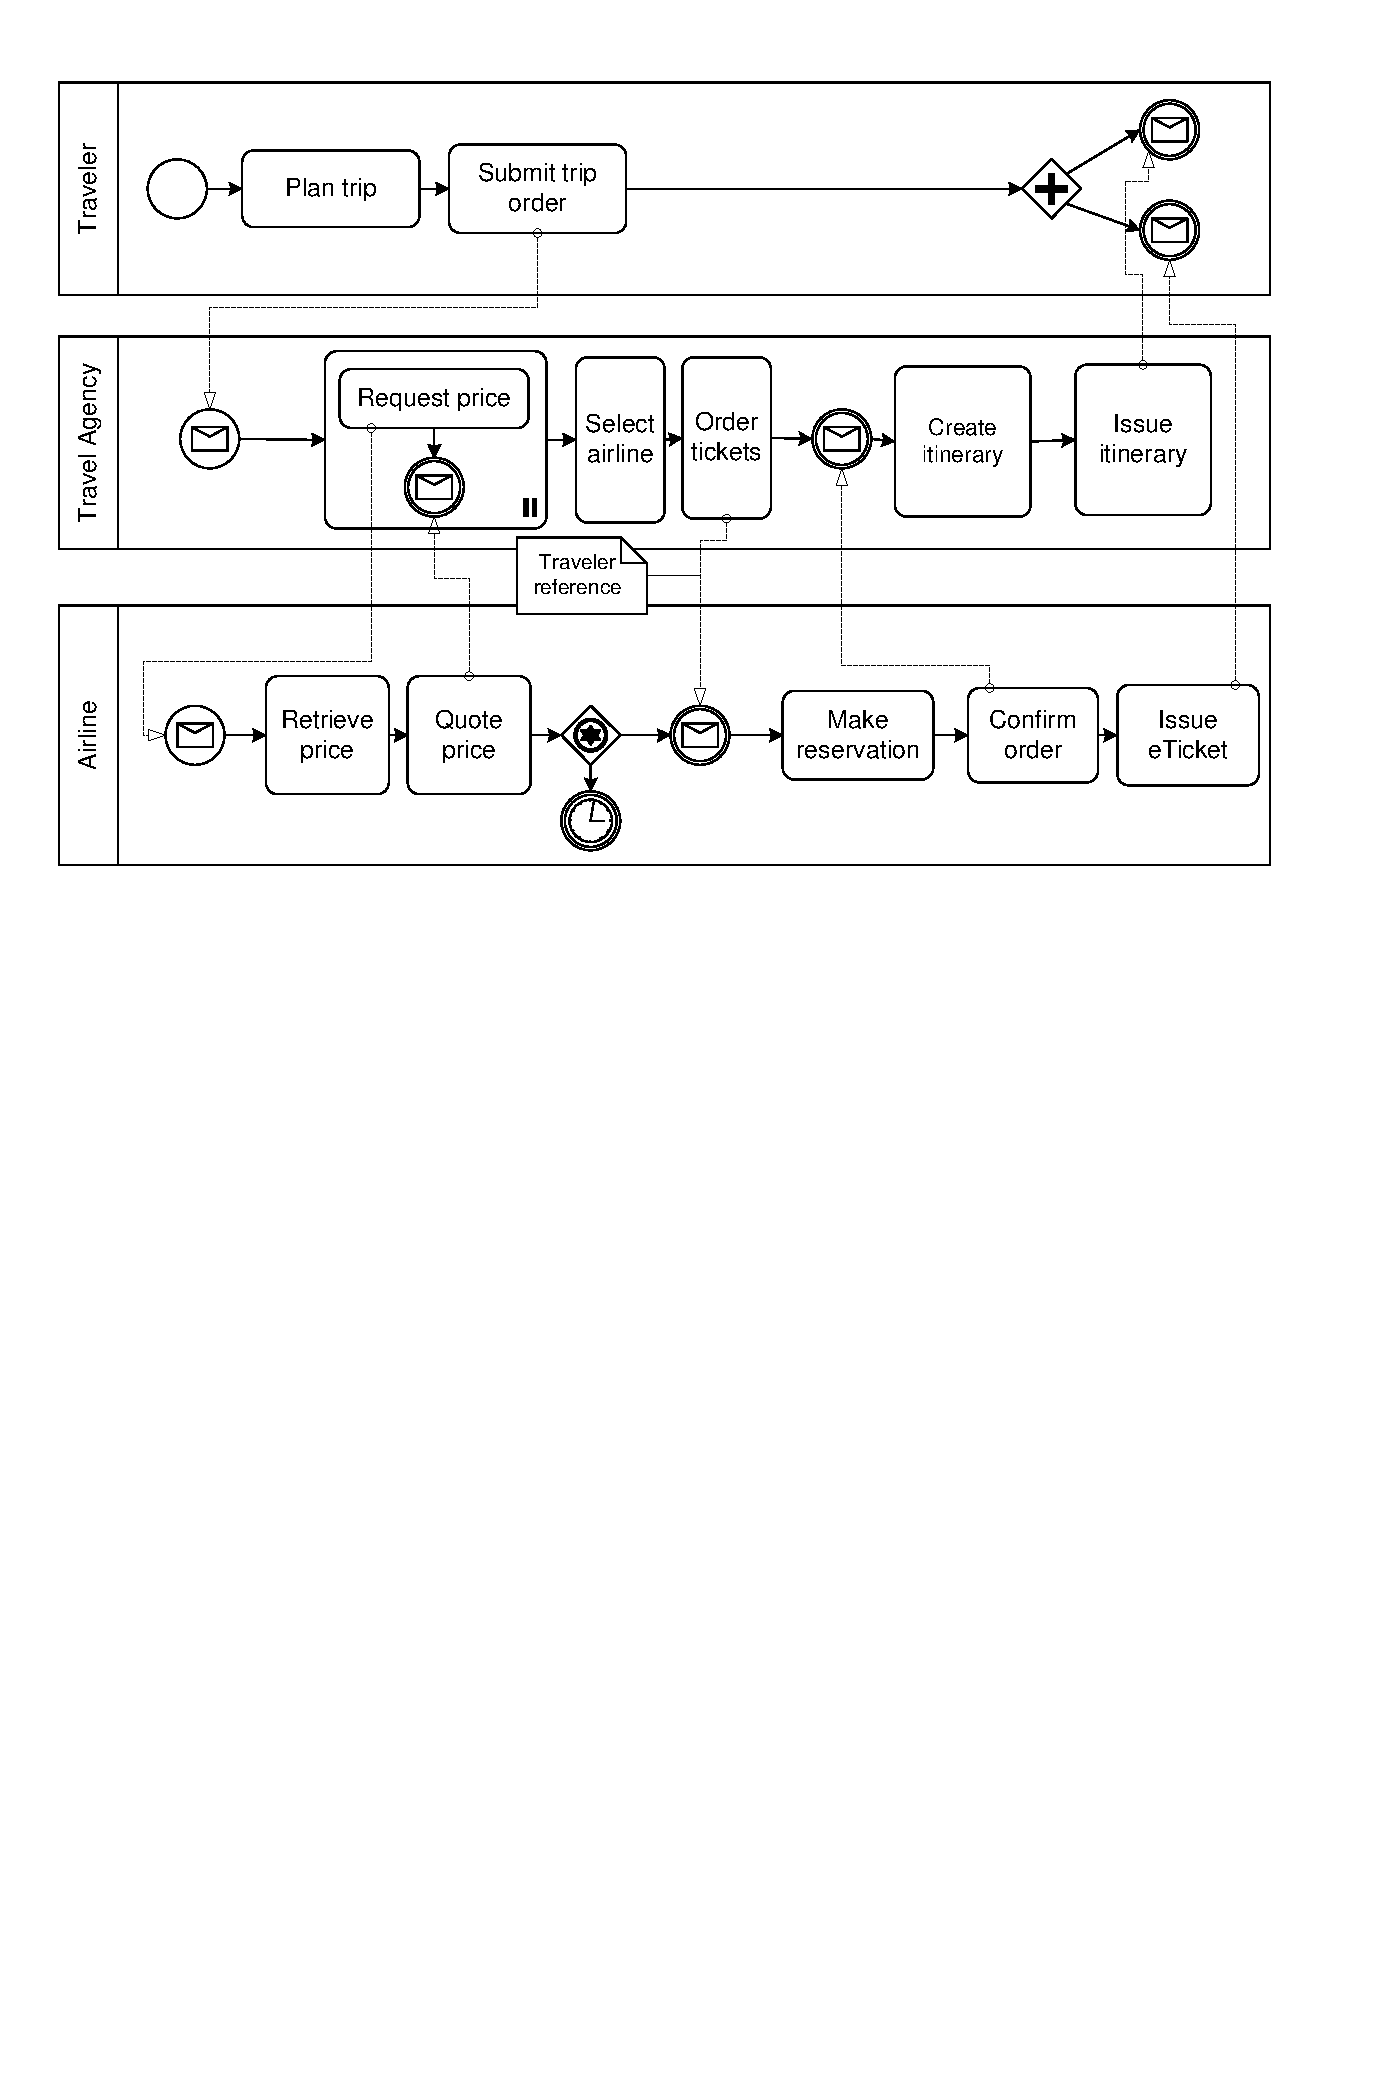
\includegraphics[width=\textwidth]{choreography.pdf}
    \caption{Beispiel-Choreographie II}
    \label{fig:AnhangsChor2}
  \end{center}
\end{figure}
\end{landscape}

%\printindex
%\bibliographystyle{alphadin}
\ifdeutsch
\bibliographystyle{bibliography/IAASde} %f"ur deutsche Texte
\else
\bibliographystyle{bibliography/IAAS} %f"ur englische Texte
\fi
\bibliography{bibliography/bibliography}
\ifdeutsch
Alle URLs wurden zuletzt am 31.05.2012 gepr\"uft.
\else
All links were last followed on March 17, 2008.
\fi

\backmatter 
\pagestyle{empty}
\renewcommand*{\chapterpagestyle}{empty}
\Versicherung
\end{document}
% Das wars, 2 Tage vorher drucken/binden lassen und abgeben nicht vegessen ;-)
